\documentclass[12pt,twoside]{report}
\usepackage[francais]{babel}
\usepackage[utf8]{inputenc}
\usepackage{graphicx}
\graphicspath{{images/}}
\usepackage[a4paper,width=150mm,top=25mm,bottom=25mm,bindingoffset=6mm]{geometry}
\usepackage{caption}
\usepackage{subcaption}
\usepackage{fancyhdr}
\usepackage{array}
\usepackage[table,xcdraw]{xcolor}
\setcounter{tocdepth}{4}
\setcounter{secnumdepth}{4}
\pagestyle{fancy}

\fancyhead{}
\fancyhead[RO,LE]{Conception et mise en place d’un système Workflow  pour l’envirenement cloud}
\fancyfoot{}
\fancyfoot[LE,RO]{\thepage}
\fancyfoot[LO,CE]{Chapter \thechapter}
\fancyfoot[CO,RE]{Zerrouki djamel}
\renewcommand{\headrulewidth}{0.4pt}
\renewcommand{\footrulewidth}{0.4pt}
%opening
\usepackage[natbib = false,
            backend = bibtex8,
            style = authoryear, 
            maxcitenames = 2,
            mincitenames = 1,
            maxbibnames = 100
            ]{biblatex}
 

\addbibresource{references.bib}
\title{
	{\textbf{Conception et mise en place d’un système Workflow  pour l’envirenement cloud}} \\   
	{$ Instituation $}\\
	{
\includegraphics{logof.PNG}}
}
\author{Zerrouki Djamel}
 
\begin{document}

\maketitle
 
\chapter*{Résumé}
..................

\chapter*{Abstrait}
......................

\chapter*{Déclaration}
.....................

\chapter*{Acknowledgements}
I want to thank...
%%%%%%%  list of Figures %%%%%%%
\listoffigures

%%%%%%%  list of Tables %%%%%%%
\listoftables

%%%%%%%  list of Contents %%%%%%%
\tableofcontents


%\appendix
\chapter{Concepts fondamentaux de cloud et de workflow }
 \fancyhead[LO,CE]{Chapter: \thechapter | Concepts fondamentaux de Cloud et de Workflow }
 	 \section{Introduction}
 	  

    Le cloud computing, traduit le plus souvent en français par " informatique dans les nuages", " informatique dématérialisée " ou encore " infonuagique ", est un domaine qui regroupe un ensemble de techniques et de pratiques consistant à accéder, en libre-service, à du matériel ou à des logiciels informatiques, à travers une infrastructure réseau (Internet). Ce concept rend possible la distribution des ressources informatiques sous forme de services pour lesquels l'utilisateur paie uniquement pour ce qu'il utilise. Ces services peuvent être utilisés pour exécuter des applications scientifiques et commerciales, souvent modélisées sous forme de workflows.
    
     
    Ce chapitre présente une introduction au cloud computing et au workflow, nécessaire pour la compréhension générale de ce mémoire.
   
   \comment{Tout d’abord, nous présentons dans la section 1.2 une introduction au paradigme du cloud computing et  sa aperçu général,  y compris sa définition, ses caractéristiques principales. Nous présentons les différents modèles de service, les différents modèles de déploiement, ainsi la sécurité dans le  cloud computing et les principaux grands fournisseurs de cloud. Par la suite, nous présentons, dans la section 1.3, une introduction au workflow et systèmes de gestion de workflow. Nous donnons le concept du workflow, sa définition.Puis la classification de système de workflow  dans la section 1.4 .   Par la suite, nous présentons, l’architecture de référence d’un système de gestion de workflows dans la section 1.5 et finalement, nous résumons l'intérêt du cloud pour les workflows.}
   
    \section{Cloud computing}
    \subsection{Concept du cloud computing}
  L'idée principale du cloud est apparue dans les années 60, où le professeur John McCarthy avait imaginé que les ressources informatiques seront fournies comme des services d’utilité publique \parencite{Garfinkel}. C'est ensuite, vers la fin des années 90, que ce concept a pris de l'importance avec l’avènement du grid computing  \parencite{Foster}. Le terme cloud est une métaphore exprimant la similarité avec le réseau électrique, dans lequel l'électricité est produite dans de grandes centrales, puis disséminée à travers un réseau jusqu'aux utilisateurs finaux. Ici, les grandes centrales sont les Datacenter, le réseau est le plus souvent celui d'Internet et l'électricité correspond aux ressources informatiques. Le cloud computing  n'est véritablement apparu qu'au cours de l’année 2006 \parencite{Vouk2008} avec l'apparition d'Amazon \ac{ec2}. C'est en 2009 que la réelle explosion du cloud survint avec l'arrivée sur le marché de sociétés comme Google (Google App Engine), Microsoft (Microsoft Azure), IBM (IBM Smart Business Service), Sun (Sun cloud) et Canonical Ltd (Ubuntu Enterprise cloud).Sun (Sun cloud) et Canonical Ltd (Ubuntu Enterprise cloud). D'après une étude menée par Forrester \parencite{Ried}, le marché du cloud computing  s'élevait à environ 5,5 milliards de dollars en 2008, il devrait atteindre plus de 150 milliards d'ici 2020, comme l’illustre la figure \ref{fig:tempsnip4}. 
    
    \begin{figure}[h]
    	\centering
    	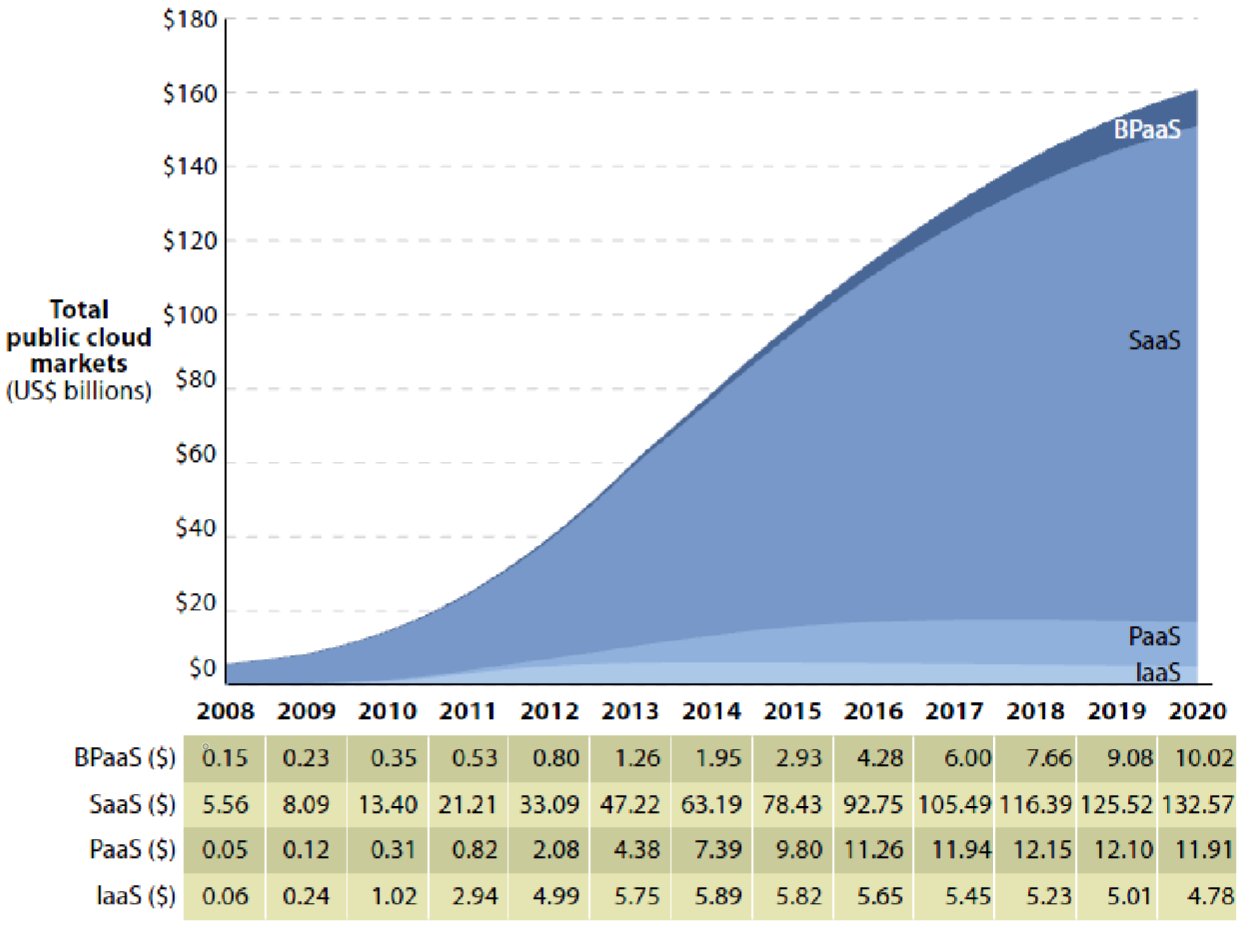
\includegraphics[width=1\linewidth]{images/tempsnip4}
    	\caption{Prévisions de la taille du marché du cloud computing  public \parencite{Ried}.}
    	\label{fig:tempsnip4}
    \end{figure}
\subsubsection{Vers une définition du cloud computing }
Beaucoup de chercheurs ont tenté de définir le cloud computing \parencite{Geelan}. La plupart des définitions attribuées à ce concept semblent se concentrer seulement sur certains aspects technologiques. L'absence d'une définition standard a généré non seulement des exagérations du marché, mais aussi des confusions. Pour cette raison, il y a eu récemment des travaux sur la normalisation de la définition du cloud computing, à l'exemple de Vaquero et coll (Vaquero, 2009) qui ont comparé plus de 20 définitions différentes et ont proposé une définition globale.  En guise de synthèse des différentes propositions données dans la littérature, nous introduisons une définition mixte, qui correspond aux différents types de cloud considérés dans les travaux réalisés dans ce mémoire.

\begin{defn}
  le cloud est comme un modèle informatique qui permet d’accéder, d’une façon transparente et à la demande, à un pool de ressources hétérogènes physiques ou virtualisées (serveurs, stockage, applications et services) à travers le réseau. Ces ressources sont délivrées sous forme de ser vices reconfigurables et élastiques, à base d’un modèle de paiement à l’usage, dont les garanties sont offertes par le fournisseur via des contrats de niveau de  \ac{als}. 
\end{defn}
%
%\begin{defn}
% Selon la définition du National Institute of Standards and Technology (NIST), le cloud computing est l'accès via un réseau de télécommunications, à la demande et en libre-service, à des ressources informatiques partagées configurables (réseaux, serveurs, stockage, applications et services), qui peuvent être provisionnées rapidement et libérées avec un effort de gestion minimale
%\end{defn}
%    
%
%\begin{defn}
%	Pour CISCO [5] le Cloud Computing est une plateforme de mutualisation informatique fournissant aux entreprises des services à la demande avec l’illusion d’une infinité de ressources. 
%\end{defn}
    \subsection{Caractéristiques principales du cloud computing}
%    Le cloud computing  possède les caractéristiques suivantes :
% 
    \subsubsection{Accès en libre-service à la demande}
     Le cloud computing offre des ressources et services aux utilisateurs à la demande. Les services sont fournis de façon automatique, sans nécessiter d’interaction humaine \parencite{Mell}. 
    \subsubsection{Accès réseau universel}
      Les services de cloud computing  sont facilement accessibles au travers du réseau, par le biais de mécanismes standard, qui permettent une utilisation depuis de multiples types de terminaux (par exemple, les ordinateur portables, tablettes, smartphones) \parencite{Mell}. 
\subsubsection{Mutualisation de ressources (Pooling)}
 Les ressources du cloud peuvent être regroupées pour servir des utilisateurs multiples, pour lesquels des ressources physiques et virtuelles sont automatiquement attribuées \parencite{Mell}. En général, les utilisateurs n’ont aucun contrôle ou connaissance sur l’emplacement exact des ressources fournies. Toutefois, ils peuvent imposer de spécifier l’emplacement à un niveau d’abstraction plus haut.
   \subsubsection{Scalabilité et élasticité} 
   Des ressources supplémentaires peuvent être automatiquement mises à disposition des utilisateurs en cas d’accroissement de la demande (en réponse à l'augmentation des charges des applications) \parencite{Geelan}, et peuvent être libérées lorsqu’elles ne sont plus nécessaires. L’utilisateur a l’illusion d’avoir accès à des ressources illimitées à n'importe quel moment, bien que le fournisseur en définisse généralement un seuil (par exemple : 20 instances par zone est le maximum possible pour Amazon EC2).
   \subsubsection{Autonome}
    Le cloud computing  est un système autonome et géré de façon transparente pour les utilisateurs. Le matériel, le logiciel et les données au sein du cloud peuvent être 
    	automatiquement reconfigurés, orchestrés et consolidés en une seule image qui sera fournie à l’utilisateur \parencite{Wang2008}.
      \subsubsection{Paiement à l’usage}
       La consommation des ressources dans le cloud s’adapte au plus près aux besoins de l’utilisateur. Le fournisseur est capable de mesurer de façon précise la consommation (en durée et en quantité) des différents services (\ac{cpu}, stockage, bande passante,…) ; cela lui permettra de facturer l’utilisateur selon sa réelle consommation (Armbrust, 2009). 
      \subsubsection{Fiabilité et tolérance aux pannes}
       Les environnements cloud tirent parti de la redondance intégrée du grand nombre de serveurs qui les composent en permettant des niveaux élevés de disponibilité et de fiabilité pour les applications qui peuvent en bénéficier \parencite{Buyya}. 
      \subsubsection{Garantie \ac{qos} }
       Les environnements de cloud peuvent garantir \ac{qos} la qualité de service pour les utilisateurs, par exemple, la performance du matériel, comme la bande passante du processeur et la taille de la mémoire \parencite{Wang2008}. 
       
    	  \subsubsection{Basé-SLA}
    	   Les clouds sont gérés dynamiquement en fonction des contrats d’accord de niveau de service (SLA)  \parencite{Buyya} entre le fournisseur et l’utilisateur. Le SLA définit des politiques, telles que les paramètres de livraison, les niveaux de disponibilité, la maintenabilité, la performance, l'exploitation, ou autres attributs du service, comme la facturation, et même des sanctions en cas de violation du contrat. Le SLA permet de rassurer les utilisateurs dans leur idée de déplacer leurs activités vers le cloud, en fournissant des garanties de QoS. 
    	Après avoir présenté les caractéristiques essentielles d’un service cloud, nous présentons, brièvement, dans la section suivante, quelques technologies connexes aux clouds.
    	
 
\subsection{Technologies connexes }
Le cloud computing  utilise des technologies telles que la virtualisation, l'architecture orientée services et les services web. Le cloud est souvent confondu avec plusieurs paradigmes informatiques, tels que le Grid computing, l’Utility computing  et l’Autonomic computing, dont chacun partage certains aspects avec le cloud computing. La figure \ref{fig:34-0} montre la convergence des technologies qui ont contribué à l'avènement du cloud computing. 

\begin{figure}[H]
	\centering
	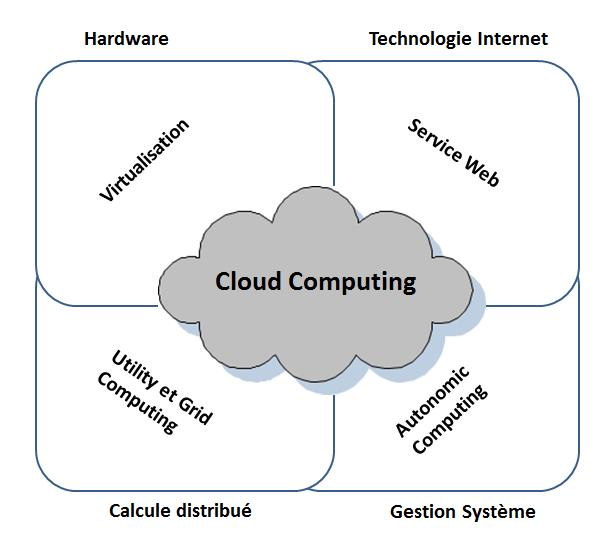
\includegraphics[width=0.5\linewidth]{images/34-0}
	\caption{ Convergence des différentes avancées menant à l'avènement du cloud computing.\parencite{cloudComputing}}
	\label{fig:34-0}
\end{figure}



\subsubsection{Grid computing: }    Le grid computing  est un paradigme de calcul réparti qui coordonne des ressources autonomes et géographiquement distribuées pour atteindre un objectif de calcul commun. Le grid est basé sur le partage dynamique des ressources entre des participants, des organisations et des entreprises dans le but de pouvoir les mutualiser, et faire ainsi exécuter des applications scientifiques, qui sont généralement des calculs intensifs ou des traitements de très gros volumes de données. Le cloud computing  est similaire au grid computing :les deux adoptent le concept d’offrir les  ressources sous forme de services. Toutefois, ils sont différents dans leur finalité : tandis que la technologie des grilles vise essentiellement à permettre à des groupes différents de partager l’accès en libre service à leurs ressources, le cloud a pour objectif de fournir aux utilisateurs des services « à la demande », sur le principe du « paiement à l’usage ». De plus le cloud  exploite les technologies de virtualisation à plusieurs niveaux (matériel et plateforme d'application) pour réaliser le partage et l'approvisionnement dynamique des ressources \parencite{meriem2012placement}.
\subsubsection{Utility computing  (informatique utilitaire): }  L’utility computing  est simplement une délocalisation d'un système de calcul ou de stockage. Il présente un modèle d’affectation des ressources à la demande et facturation des utilisateurs en fonction de leur usage. Le cloud computing  peut être perçu comme une réalisation de l'informatique utilitaire. Il adopte un système de tarification basé sur l'utilité, entièrement pour des raisons économiques. Avec l'approvisionnement des ressources à la demande et le paiement à l’usage, les fournisseurs de services peuvent maximiser l'utilisation des ressources et minimiser leurs coûts d'exploitation.

\subsubsection{L'autonomic computing: }   L’autonomic computing  vise à construire des systèmes  informatiques capables de s’auto-administrer en s’adaptant à des changements  internes et externes sans intervention humaine. Le but de l'informatique autonome est de surmonter la complexité de la gestion des systèmes informatiques d'aujourd'hui. Bien que le cloud computing  présente certaines caractéristiques autonomes, telles que l’approvisionnement automatique des ressources, son objectif est de diminuer le coût des ressources, plutôt que de réduire la complexité du système \parencite{yassa2014allocation}.

\subsubsection{Virtualisation: }   La virtualisation est une technologie qui fait abstraction des détails du matériel physique et fournit des ressources virtualisées pour les applications de haut niveau. En effet, la virtualisation regroupe l’ensemble des techniques matérielles ou logicielles permettant de faire fonctionner, sur une seule machine physique, plusieurs configurations informatiques (systèmes d’exploitation,…), de sorte à former plusieurs machines virtuelles, qui reproduisent le comportement des machines physiques. La virtualisation constitue le socle du cloud computing, car elle offre la possibilité de mettre en commun des ressources informatiques à partir de clusters de serveurs, et ainsi d’affecter ou réaffecter dynamiquement des machines virtuelles aux applications à la demande. La figure \ref{fig:virtualisation}. montre l’architecture en couches de la technologie de virtualisation. Le  \ac{vmm} en français moniteur de machine virtuelle ,  également appelé hyperviseur, partitionne la ressource physique du serveur physique sous-jacente en plusieurs machines virtuelles  différentes, chacune fonctionnant sous un système d'exploitation distinct et une pile de logiciels utilisateur \parencite{bouchhima2006modelisation}.

 
\begin{figure}[H]
	\centering
	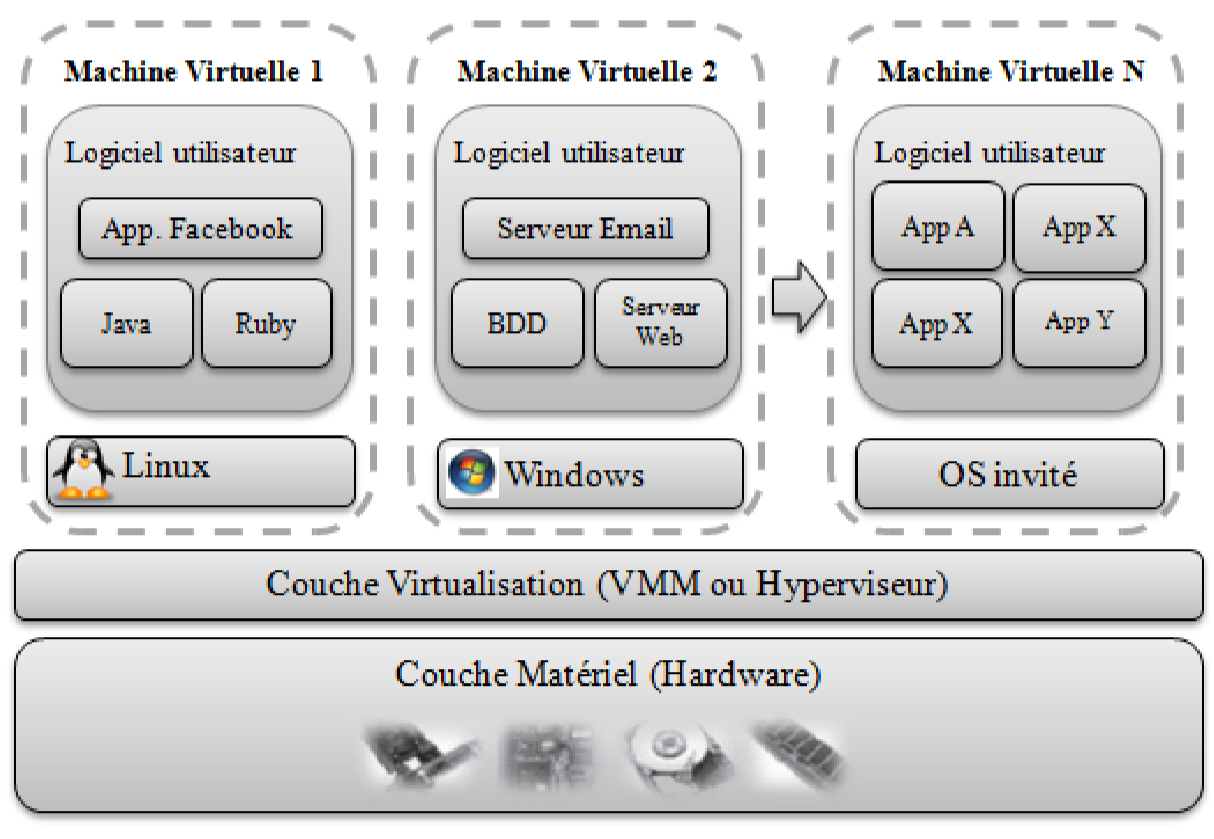
\includegraphics[width=1\linewidth]{images/virtualisation}
	\caption{ Une architecture en couches de la technologie de virtualisation. }
	\label{fig:virtualisation}
\end{figure}

 














%\subsection{Modèles du cloud computing  }
\subsection {Modèles de service du cloud computing}  
\ac{xaas} représente la base du paradigme du cloud computing, où X représente un service tel qu’un logiciel, une plateforme, une infrastructure, un Business Process \ac{bpaas}, etc. Nous présentons, dans cette section,  quatre  modèles de services \parencite{Rimal}, à savoir: (1) Logiciel en tant que services \ac{saas},  où le matériel, l’hébergement, le framework d’application et le logiciel sont dématérialisés, (2) Plateforme en tant que service \ac{paas}, où le matériel, l’hébergement et le framework d’application sont dématérialisés, (3) Infrastructure en tant que service \ac{iaas} et (4) Matériel en tant que service \ac{haas}, où seul le matériel (serveurs) est dématérialisé dans ces deux derniers cas. La figure \ref{fig:capture5} montre le modèle classique et les différents modèles de service de cloud
\begin{figure}[H]
	\centering
	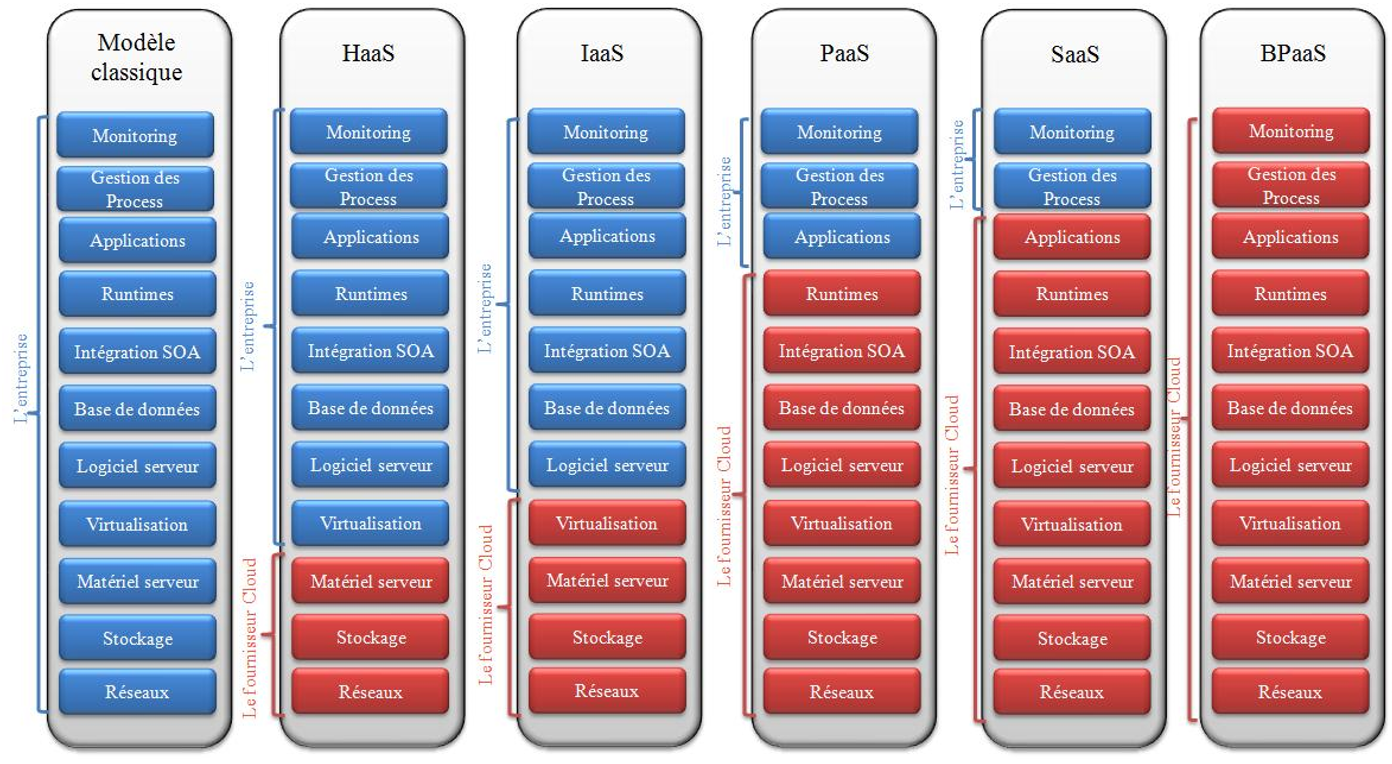
\includegraphics[width=1\linewidth]{Capture5}
	\caption{Les services XaaS du cloud computing}
	\label{fig:capture5}
\end{figure}

\subsubsection{Software as a Service (SaaS)}

Ce modèle de service est caractérisé par l’utilisation d’une application partagée qui fonctionne sur une infrastructure Cloud. L’utilisateur accède à l’application par le réseau au travers de divers types de terminaux (souvent via un navigateur web). L’administrateur de l’application ne gère pas et ne contrôle pas l’infrastructure sous-jacente (réseaux, serveurs, applications, stockage).  Il ne contrôle pas les fonctions de l’application à l’exception d’un paramétrage de quelques fonctions utilisateurs limitées. On prend comme exemple les logiciels de messagerie au travers d’un navigateur comme Gmail ou Yahoo mail. 

\subsubsection{ Platform as a Service (PaaS)}

L’utilisateur a la possibilité de créer et de déployer sur une infrastructure Cloud PaaS ses propres applications en utilisant les langages et les outils du fournisseur. L’utilisateur ne gère pas ou ne contrôle pas l’infrastructure Cloud sous-jacente (réseaux, serveurs, stockage) mais l’utilisateur contrôle l’application déployée et sa configuration. Comme exemple de PaaS, on peut citer un des plus anciens -IntuitQuickbase- qui permet de déployer ses applications bases de données en ligne ou -\ac{gae}- pour déployer des services Web. 

Dans ces deux cas l’utilisateur de ces services n’a pas à gérer des serveurs ou des systèmes pour déployer ses applications en ligne et dimensionner des ressources adaptées au trafic.
\subsubsection{Infrastructure as a Service (IaaS)}

L’utilisateur loue des moyens de calcul et de stockage, des capacités réseau et d’autres ressources indispensables (partage de charge, pare-feu, cache). L’utilisateur a la possibilité de déployer n’importe quel type de logiciel incluant les systèmes d’exploitation. L’utilisateur ne gère pas ou ne contrôle pas l’infrastructure Cloud sous-jacente mais il a le contrôle sur les systèmes d’exploitation, le stockage et les applications. Il peut aussi choisir les caractéristiques principales des équipements réseau comme le partage de charge, les pare-feu, etc. L’exemple emblématique de ce type de service est Amazon Web Services qui fournit du calcul (EC2), du stockage (S3, EBS), des bases de données en ligne (SimpleDB) et quantité d’autres services de base. Il est maintenant imité par de très nombreux fournisseurs.
	  
 
\subsection { Modèles de déploiement}  

Selon la définition du cloud computing  donnée part le \ac{nist} \parencite{Mell}, il existe quatre modèles de déploiement des services de cloud, à savoir : cloud privé, cloud communautaire, cloud public et cloud hybride, comme illustré dans la figure \ref{fig:cloudmd}.
 
\subsubsection{Cloud privé :}
	 L’ensemble des ressources d’un cloud privé est exclusivement mis à disposition d’une entreprise ou organisation unique. Le cloud privé peut être géré par l’entreprise elle même (cloud privé interne) ou par une tierce partie (cloud privé externe). Les ressources d’un cloud privé se trouvent généralement dans les locaux de l’entreprise ou bien chez un fournisseur de services. Dans ce dernier cas, l’infrastructure est entièrement dédiée à l’entreprise et y est accessible via un réseau sécurisé (de type \ac{vpn}).  L’utilisation d’un cloud privé permet de 	garantir, par exemple, que les ressources matérielles allouées ne seront jamais partagées par deux clients différents. 
	
\subsubsection{Cloud communautaire}
	 L’infrastructure d’un cloud communautaire est partagée par plusieurs organisations indépendantes ayant des intérêts communs. L’infrastructure peut être gérée par les organisations membres ou par un tiers. L’infrastructure peut être située, soit au sein des dites organisations, soit chez un fournisseur de services. 
\subsubsection{Cloud public}
	L’infrastructure d’un cloud public est accessible à un large public et appartient à un fournisseur de services. Ce dernier facture les utilisateurs selon la consommation et garantit la disponibilité des services via des contrats SLA. 
\subsubsection{Cloud hybride}
	 L’infrastructure d’un cloud hybride est une composition de plusieurs clouds (privé, communautaire ou public). Les différents clouds composant l’infrastructure restent des entités uniques, mais sont reliés par une technologie standard ou propriétaire permettant ainsi la portabilité des données ou des applications déployées sur les différents clouds.  

\begin{figure}[H]
	\centering
	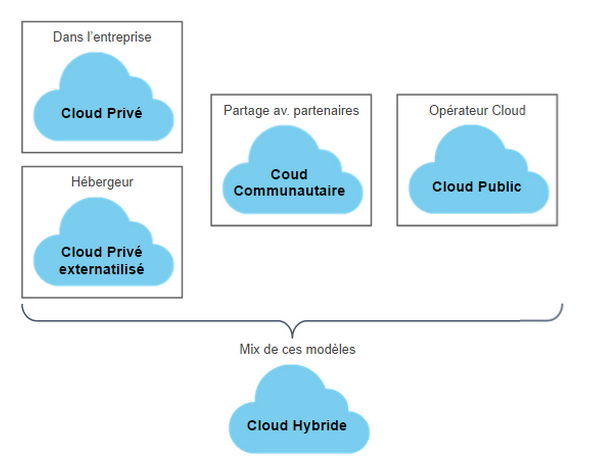
\includegraphics[width=0.5\linewidth]{Cloud_MD}
	\caption{Modèles de déploiement du cloud computing }
	\label{fig:cloudmd}
\end{figure}
 
%
%\subsection{Cloud computing et sécurité}
%Toutes les enquêtes montrent que la sécurité est la préoccupation majeure des organisations dans le processus d’adoption des technologies Cloud. Les questions sont nombreuses comme par exemple :
%
%\begin{itemize}
%
%\item Quelle confiance peut-on avoir dans le stockage des données à l’extérieur de l’entreprise ?
%\item Quels sont les risques associés à l’utilisation de services partagés ?
%\item Comment démontrer la conformité des systèmes à des normes d’exploitation ?
%\end{itemize}
%
%Les infrastructures Cloud sont de gigantesques systèmes complexes. Ils peuvent cependant être réduits à un petit nombre de primitives simples qui sont instanciées des milliers de fois et à quelques fonctions communes. La sécurité du Cloud est donc un problème gouvernable moins complexe qu’il n’y parait.
%
%\subsubsection{Avantages et défis du Cloud en terme de sécurité}
%
%Le Cloud présente des avantages immédiats. D’une manière générale, le fait d’héberger des données publiques sur le Cloud réduit les risques pour les données internes sensibles. D’autre part, l’homogénéité dans la construction du Cloud en rend les tests et les audits plus simples. De même la conduite du système au travers de web services permet la mise en place  de procédures automatiques accroissant notablement la sécurité.
%
%En revanche les défis restent nombreux pour les fournisseurs.  Il faut donner confiance dans le modèle de sécurité et dans les outils de gestion qui sont proposés. Les tâches de gestion sont réalisées de manière indirecte au travers d’une interface puisque l’utilisateur n’a pas de contrôle direct sur l’infrastructure physique. Ce partage des responsabilités complique un peu les audits de sécurité.
%
%\subsubsection{Les composants sécurité d’un système de Cloud computing}
%Les différents composants qui participent à la sécurité d’un système de Cloud computing présentent les caractéristiques suivantes :
%\begin{itemize}
%	 
%\item \textbf{Service de console de gestion (Provisioning):}\\
%La mise en route et la reconfiguration des composants des systèmes sont très rapides. Il est possible de mettre en service plusieurs instances dans plusieurs centres de traitement répartis dans le monde en quelques minutes. Les reconfigurations réseau sont facilitées. En revanche, la sécurité d’utilisation de la console de gestion devient impérative (authentification multi-facteurs, connexion chiffrée, etc..)
%
%\item \textbf{Service de stockage des données:}\\
%Les avantages du stockage des données dans le Cloud dépendent des fournisseurs mais en général, ceux-ci fragmentent et répartissent les données. Celles ci sont aussi souvent recopiées dans des centres de traitement différents. Ces opérations améliorent considérablement la sécurité des données. Si leur contenu doit rester confidentiel, il convient de les chiffrer avant de les stocker.
%
%\item \textbf{Infrastructures de calcul:}\\
%Un des gros avantages du Cloud pour le développement et l’exploitation des applications réside dans la virtualisation. Elle permet de préparer des configurations maîtres sûres qu’il suffit de dupliquer pour déployer. Les défis restent la sécurisation des données dans les applications partagées et  la sécurité entre les instances garantie par les hyperviseurs.
%\item \textbf{Services de support:}\\
%La principale caractéristique du Cloud est la mise en place a priori d’une sécurité renforcée et auditable (authentification, logs, pare-feux, etc..). Il reste à traiter les risques liés à l’intégration avec les applications des utilisateurs ainsi que les processus toujours délicats de mises à jour
%\item \textbf{Sécurité périmétrique du réseau Cloud:}\\
%Ces grandes infrastructures partagées fournissent des moyens de protection au delà des capacités  d’une entreprise normale comme par exemple la protection contre les attaques DDOS (Distributed Denial Of Service). Les mécanismes de sécurité périmétriques sont généralement bien conçus (fournisseur d’identité, authentification, pare-feux,  etc..). En revanche, il reste à traiter les sujets liés à la mobilité.
%
%\end{itemize}


\subsection{Les principaux grands fournisseurs cloud pour 2019}  


Comment choisir la solution de cloud la plus adaptée à votre entreprise, quelles sont les différentes offres et les tarifs pour stocker les données informatiques sur un serveur à distance. Comparatif des principales solutions du marché.

\subsubsection{Amazon Web Services }

Avec un chiffre d’affaires de 25.65 milliards de dollar (\textbf{\underline{Zdnet.fr}}) réalisé en 2018, le géant de l’IaaS considère 2019 comme une année d’investissement afin d’accélérer le développement de sa technologie et renforcer sa force de vente. En ce début de 2019, \ac{aws} est le leader incontesté dans le domaine de l’IaaS \parencite{cloud2019}.

\subsubsection{Microsoft Azure}
Le service cloud, Microsof Azure a réalisé un chiffre d’affaires annuel de 11 milliards de dollar. En 2019, le service cloud Microsoft Azure vient en deuxième position derrière AWS (IaaS et PaaS). A la différence d’AWS, Microsoft opère plutôt dans le commercial cloud et propose un service très diversifié grâce à une plateforme familiarisée auprès des utilisateurs \parencite{cloud2019}.


\subsubsection{Google Cloud Plateform}
L’année 2018 a été particulièrement fructueuse chez le service cloud de Google. Avec un chiffre d’affaires de près 4 milliards de dollar, l’entreprise a décroché en 2018 les contrats les plus importants dans le secteur. Pour 2019, elle va constituer un véritable contrepoint à AWS et à Microsoft même si l’entreprise a toujours du mal à publier convenablement ses rapports financiers jusqu'à présent \parencite{cloud2019}.

\subsubsection{IBM}
Très présent dans le monde du multicloud et du cloud hybride, il dispose actuellement d’un chiffre d’affaires de 12.2 milliards de dollar. Même s’il reste un peu derrière AWS et Microsoft, il est en train de se focaliser sur le développement d’une plateforme capable de gérer plusieurs outils d’intelligence artificielle pour les principaux fournisseurs cloud. En plus, l’acquisition de Red Hat est un signal fort pour le cloud hybride \parencite{cloud2019}.

 
 
%%%%%%%%%%%%%%%%%%%%%%%%%%%%              Workflow et systèmes de gestion de workflows 
%%%%%%%%%%%%%%%%%%%%%%%%%%%%

 \section{Workflow}
 	 
 	 \subsection{Introduction au Workflow }
 	 
 	 
 	 Un Workflow est la modélisation et la gestion assistée par ordinateur de l’accomplissement des tâches composant un processus administratif ou industriel, en interaction avec divers acteurs (humains, logiciels, ou matériels) invoqués \parencite{Courtois}.  Outil informatique d’origine industrielle, le Workflow est l’adaptation de la GED24 adjoint de la faculté à gérer l’échange de messages. Le Workflow propose des solutions d’optimisation et de rationalisation des flux d’informations ; que ces informations soient associées à des documents, des procédures ou des messages complémentant les systèmes de gestion électronique de documents et d’informations.
 	 
 	 A l’heure actuelle plus de 250 Systèmes de Gestion de Workflow (WFMS) sont utilisés ou en développement. Cela signifie que le terme « gestion de Workflow » n’est pas simplement une nouvelle expression à la mode. Ce phénomène de gestion de processus (Workflow) aura certainement un fort impact sur la génération suivante de systèmes informatiques \parencite{Courtois}. 
 	 
 \subsection{Origines} 
 	 Il est intéressant de considérer l’évolution des systèmes informatiques au cours des quatre dernières décennies \parencite{VanderAalst} pour prendre conscience de la pertinence d’une gestion électronique de processus (Workflow) et apprécier l’impact de la gestion de Workflow dans un avenir proche.
 	 
 	  La Figure \ref{fig:wfmchistory} présente le phénomène de gestion de Workflow dans une perspective historique. Cette figure décrit l’architecture d’un système informatique classique en termes de composants. Dans les années soixante, un système informatique était composé d’un certain nombre d’applications autonomes. Pour chacune de ces applications une interface utilisateur et un système de base de données spécifique étaient développés, chaque application possédait donc ses propres routines pour interagir avec l’utilisateur, stocker et récupérer les données. Dans les années soixante-dix, le développement des \ac{sgbd} a permis d’extraire les données des applications. En utilisant les SGBD, les applications ont ainsi été libérées du fardeau de la gestion de données. Dans les années quatre vingts, l’apparition de systèmes de gestion d’interface utilisateur \ac{uims} a permis aux développeurs d’application d’extraire l’interaction avec les utilisateurs des applications.
 	  
 	   Enfin, les années quatre-vingt-dix sont marquées par l’apparition de logiciels de Workflow, permettant aux développeurs d’application d’extraire les procédures de travail des applications. La Figure \ref{fig:wfmchistory} fait apparaître le système de gestion de Workflow comme une composante générique pour représenter et manipuler les processus d’entreprise \footnote[1]{\samepage Les procédures d’entreprise représentent l’organisation et la politique de l’entreprise pour atteindre certains objectifs \parencite{WFMC11} }. 
 	  
 	  Ainsi, à l’heure actuelle, beaucoup d’organisations commencent à considérer l’utilité d’outils avancés pour soutenir la conception et l’exécution de leurs processus d’entreprise.
 	 
 	 
 	 
\begin{figure}[h]
	\centering
	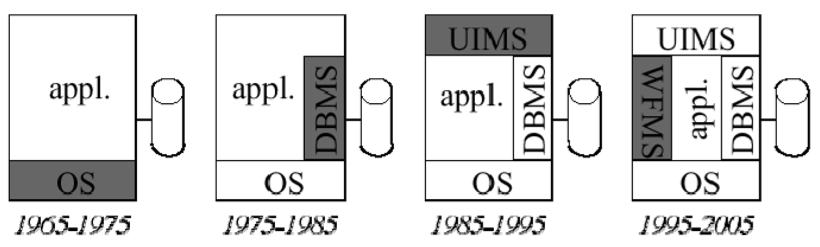
\includegraphics[width=0.7\linewidth]{images/wfmcHistory}
	\caption{Les systèmes de gestion de Workflow dans une perspective historique }
	\label{fig:wfmchistory}
\end{figure}
 	 
 	 
 	 \subsection{Définitions et terminologies }
 	 
 	 Les définitions sont, pour la majorité, issues de la Coalition de Gestion de Workflow "\ac{wfmc}". La WfMC a été fondée en 1993 par un regroupement d’industriels de l’informatique, de chercheurs et d’utilisateurs, associée à l’essor du développement des Workflows. Cette coalition a pour but de promouvoir les Workflow et d’établir des standards pour les \ac{wfms}. Elle a en particulier publié un glossaire de référence contenant les terminologies employées dans ce domaine \parencite{WFMC11}. Ces standards servent notamment à résoudre les problèmes d’interopérabilité entre systèmes Workflow mais également à définir les caractéristiques fondamentales de ces systèmes. Les documents publiés par la WfMC, qui couvrent plusieurs aspects, peuvent être considérés comme des références en la matière. 
 	
 	\subsection{Définitions de base du Workflow } 
 	 
 	 Le sens du mot Workflow peut varier en fonction du contexte. Pour plus de clarté, les définitions les plus communément admises sur les concepts et les termes du Workflow sont rappelées ci dessous. Ces définitions sont principalement issues du \ac{wfmc-tc} \parencite{WFMC11}, dont il existe une traduction à usage francophone \parencite{WFMC11}. L’idée première du Workflow est donc de séparer les processus, les ressources et les applications, afin de se recentrer sur la logistique des processus travail et non pas sur le contenu des tâches individuelles. Un Workflow est donc le lien entre ces trois domaines comme précise la Figure \ref{fig:environnementswf}. 
 	 
 	 
 	 
 	 
 	 
 	 
 	 
\begin{figure}[H]
	\centering
	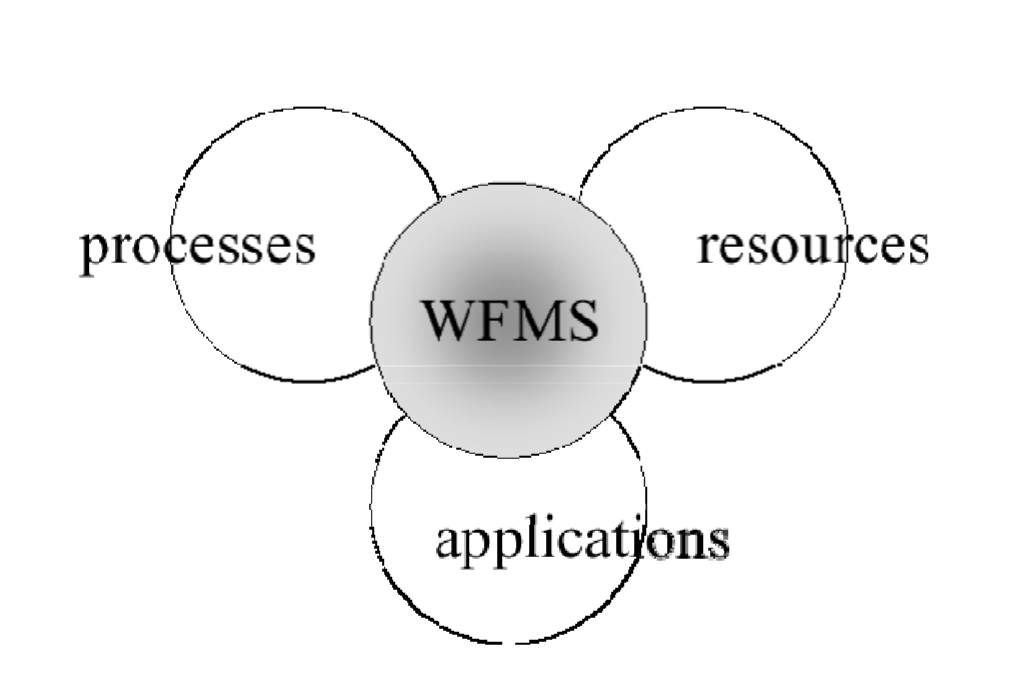
\includegraphics[width=0.4\linewidth]{images/Environnementswf}
	\caption{ Environnement du système Workflow \parencite{zacharewicz2006environnement}}
	\label{fig:environnementswf}
\end{figure}
 	 
 	 
 	 
 	 
 	 \subsubsection{Définition d’un Workflow }
 	 
 	 
 	 Le Workflow est une technologie informatique ayant pour objectif la gestion des processus d’organisations ou d’entreprises : les termes suivants sont également employés pour qualifier cette technologie « Système de Gestion Electronique de Processus », « Gestion de Workflow » ou « Gestion de processus » \parencite{Courtois}. 
 	 
 	 Le Workflow est l’ensemble des moyens mis en œuvre pour automatiser et gérer les processus d’une organisation. Cette gestion est rendue possible par la représentation sous forme d’un modèle, de tout ou partie des processus considérés. Le Workflow doit ensuite transcrire les modèles obtenus en une forme exécutable. Enfin, ces modèles sont exécutés et gérés. Il est ainsi possible de suivre l’évolution de leur état au fil du temps. La gestion de processus inclut également, au cours de l’exécution, la coordination et la synchronisation des différents acteurs des processus en fonction de l’état actuel des modèles.
 	 
 	 Pour résumer, la Gestion de Processus permet donc d’attribuer à chacun et au bon moment, les tâches dont il a la responsabilité et de mettre à disposition les applications, les outils et les informations nécessaires pour leurs réalisations. Dans un contexte d’acteurs humains, le Workflow permet de décharger les acteurs de certaines tâches de gestion administrative, en leur laissant la possibilité de se concentrer sur les contenus des tâches techniques en rapport avec leurs compétences. De plus, le Workflow donne la possibilité d’effectuer une activité de monitoring sur le déroulement des Workflow de l’entreprise, permettant en particulier de connaître, en fonction de la date, l’état des activités, des acteurs, des applications et quelles sont les prochaines activités planifiées. 
 	 
 	 En synthèse, La WfMC présente le Workflow comme l’automatisation d’un processus d’entreprise, en intégralité ou en partie, pendant laquelle on définit les transmissions des documents, de l’information ou des tâches d’un participant à un autre pour agir, selon un jeu de règles procédurales \parencite{WFMC11}. Un Système Workflow définit, gère et exécute des procédures en exécutant des programmes dont l’ordre d’exécution est prédéfini dans une représentation informatique de la logique de ces procédures - les Workflow \parencite{WFMC11}. 
 	 
 	 \comment{
 	 \subsubsection{ Méta Modèle basique }
 	 Le Workflow est basé sur un ensemble de concepts. La WfMC \parencite{WFMC11} a proposé un méta modèle de Définition de Procédures, qui identifie les concepts de haut niveau dans la Définition de Processus. Ce modèle permet de mieux appréhender les concepts et leurs interrelations. 
 	 
 	 
 	 
 	 
\begin{figure}[h]
	\centering
	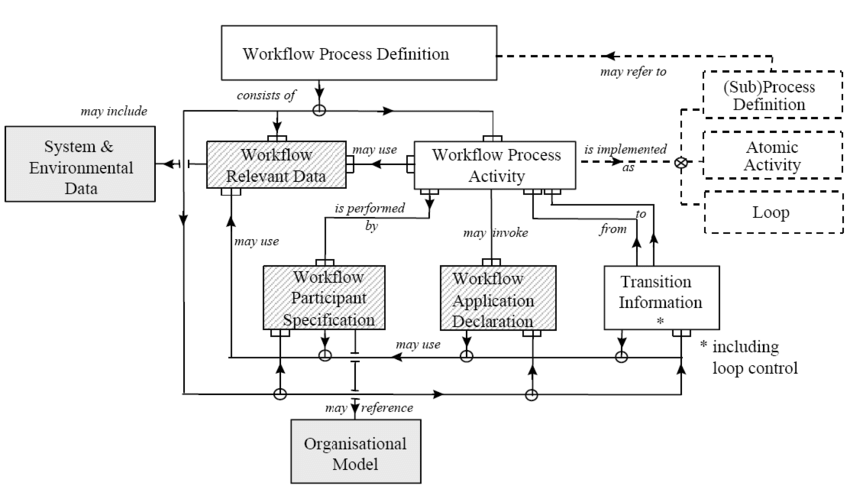
\includegraphics[width=1\linewidth]{images/MetaMWFMC11-99}
	\caption{Méta modèle Workflow pour la définition de Processus \parencite{WFMC11}}
	\label{fig:metamwfmc11-99}
\end{figure}
 	 
 	 Le méta modèle, présenté Figure \ref{fig:metamwfmc11-99}, identifie un ensemble d’objets fondamentaux qui entrent dans la définition d’un processus géré par un système Workflow, et que nous allons définir et commenter dans les paragraphes suivants. Remarquons que le méta modèle peut être enrichi par les développeurs de systèmes, il peut également être utilisé à des fins d’échanges entre différents systèmes Workflow.
 	 
 	}
 	 \subsubsection{Dimensions}
 	 Associé aux définitions précédentes, il a été défini une représentation tridimensionnelle des systèmes Workflow \parencite{VanderAalst} (Figure \ref{fig:dimensionswf}). 
 	 
 	 
\begin{figure}[H]
	\centering
	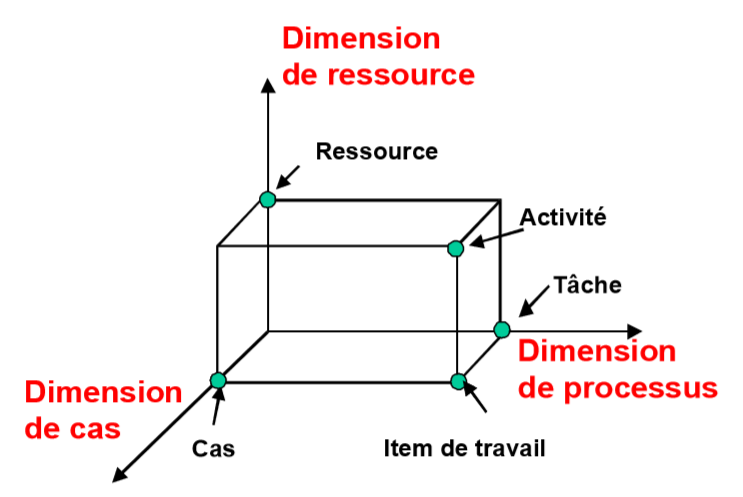
\includegraphics[width=0.49\linewidth]{images/DimensionsWF}
	\caption{ Dimensions des systèmes Workflow }
	\label{fig:dimensionswf}
\end{figure}
 	 La Figure \ref{fig:dimensionswf} donne une représentation tridimensionnelle d’un Workflow : avec une dimension de cas, une dimension de processus et une dimension de ressource. La dimension de cas représente l’instanciation du Workflow, chaque cas est un modèle à simuler et traiter individuellement. Les cas ne s’influencent donc pas directement. Ils peuvent éventuellement s’influencer indirectement via les ressources et les données. Le processus de Workflow est spécifié dans la dimension de processus, c’est-à-dire, la définition des tâches et de leur enchaînement. Enfin, dans la dimension de ressource, les ressources sont regroupées en rôles et en unités organisationnelles. En résumé, nous pouvons donc visualiser un certain nombre de termes Workflow dans la vue tridimensionnelle de la Figure \ref{fig:dswf} . En particulier, une entité de travail est définie par la coordonnée cas + tâche et une activité par le cas + la tâche + la ressource.
 	  Cette représentation met en relief la gestion de Workflow comme le lien entre les cas, les tâches et l’organisation. 
 	 
 	 \subsection{Description des Systèmes Workflow }
 	 Après avoir présenté la terminologie Workflow, il est maintenant possible de présenter le principe de fonctionnement des systèmes Workflow. A un haut niveau, ce type de système est composé de trois parties fonctionnelles \parencite{WFMC11}. La Figure \ref{fig:dswf} illustre un Système de gestion de Workflow et les relations entre ses différentes fonctions. 
 	 
 	 
 	 
 
\begin{figure}[H]
	\centering
	\includegraphics[width=0.7\linewidth]{"dswf"}
 
	\caption{Caractéristiques du système Workflow}
	\label{fig:dswf}
\end{figure}
 	 \subsubsection{ Build time }
 	 
 	 Cette première phase permet la définition et la modélisation des procédures Workflow, elle est nommée build time. Elle est principalement composée d’un outil permettant la modélisation des Workflow dans un formalisme existant ou propriétaire à partir d’une analyse de procédures d’entreprises, il est à noter que les outils actuels préfèrent une description graphique. Un deuxième composant transcrit les modèles obtenus dans une définition des procédures « exécutable », c’est à dire compréhensibles par la partie chargée de l’exécution (simulateur du run time). Certains systèmes permettent en retour de la partie run time des modifications dynamiques de la structure de définition de procédures comme indiqué sur la Figure \ref{fig:dswf}. 
 	  	 \subsubsection{ Run time }
 	 L’environnement d’exécution (ou run time) a l’entière gestion des modèles de Workflow établis dans la première partie. Cette gestion comprend l’exécution des Workflow avec un simulateur mais aussi la distribution des tâches aux rôles appropriés en cours d’exécution, la mise à disposition de l’ensemble des données et outils nécessaires, la supervision et le contrôle, etc.
 	 
 	 Plus en détails, cette partie se décline en sous composants, introduits ci dessous : Le Moteur de Workflow (Workflow Engine) qui est chargé de la Gestion des Procédures à travers la simulation de leurs évolutions. 
 	 
 	 Le gestionnaire des listes de tâches (Worklist Handler), chargé de distribuer les activités dans les listes des acteurs en fonction de leurs rôles. 
 	 
 	 Les listes de tâches (Worklists), qui sont les listes associées à chaque rôle dans lesquelles le moteur place les tâches à réaliser. Les tâches sont classées par priorité ou par date avec les données et les outils à utiliser de façon appropriée. 
 	 
 	 
 	 Les outils d’administration et de contrôle (Workflow Process Monitoring) suivent le déroulement des procédures Workflow, elles peuvent fournir l’état actuel des composantes du Workflow et donner l’ordre de modifier le modèle de procédures.
 	 
 	  	  	 \subsubsection{ Utilisateurs, outils et applications }
 	  	  	 La troisième phase concerne l’ensemble des outils et des fonctions d’API (Application Programming Interface) qui permettent au système Workflow de s’interfacer avec des ressources humaines, des applications informatiques extérieures et d’autres systèmes Workflow. 
 	  	  	 
 	 
 	 
 	 
 
 	 	 \comment{ 
 	 
 	\subsection{Concepts et Terminologie Workflow fondamentaux } 
 	 
 	 Les principaux termes associés aux Workflow proposés par la WfMC \parencite{WFMC11} sont présentés dans le diagramme du méta modèle Workflow ci-dessus, ce diagramme permet également de mettre en évidence leurs interrelations. Les termes présentés ci-dessous en français avec la traduction anglaise originale associée, couvrent les notions plus importantes appartenant au Workflow et à son lexique \parencite{WFMC11}. 
 	 
 	 \subsubsection{Procédure Workflow (Workflow Process) }
 	 
 	 Une procédure Workflow est une procédure contrôlée par un Workflow. Une procédure est composée de plusieurs activités enchaînées pour représenter un flux de travail. Une procédure possède une structure hiérarchique et modulaire, en l’occurrence une procédure peut donc être composée de sous procédures et d’activités. Les sous-procédures peuvent être composée elles mêmes de procédures manuelles ou de procédures Workflow.
 	 
 	 
 	 \subsubsection{Activité (Process Activity) }
 	 Une activité est une étape d’un processus au cours de laquelle une action élémentaire est exécutée. On désigne par « action élémentaire » (ou tâche) une activité qui n’est plus décomposable en sous-procédures. La WfMC distingue une « activité manuelle », qui n’est pas contrôlée par le système Workflow, et une « activité Workflow » qui est sous le contrôle du Workflow. Un exemple d’une activité manuelle est l’ouverture d’un courrier. Une activité Workflow peut être le remplissage d’un formulaire électronique. Il existe donc des exemples d’activités manuelles intégrables dans un Workflow. 
 	 
 	 \parencite{VanderAalst} présente l’activité Workflow comme l’intersection entre une ressource humaine ou matérielle et un bon de travail dans le cadre de l’exécution d’une tâche. Dans cette représentation, une ressource du modèle organisationnel est donc exigée pour qu’une tâche puisse être instanciée en activité et allouée à un participant de Workflow. 
 	 
 	 
 	 
 	  	 \subsubsection{ Acteur, Ressource (Workflow Participant) }
 	 
 	Un acteur est une entité du modèle organisationnel participant à l’accomplissement d’une procédure. L’acteur est chargé de réaliser les activités qui lui sont attribuées via le(s) rôle(s) qui lui sont définis dans le modèle organisationnel. Les autres dénominations courantes dans la littérature de cette entité sont « ressource », « agent », « participant » ou « utilisateur ». L’acteur peut être une ressource humaine ou matérielle (machine, périphérique informatique…).
 	 
 	 Les ressources sont organisées en classes dans le modèle organisationnel. Ces classes sont des groupes de ressources possédant des propriétés communes. Une classe est basée sur :
 	 
 	 \textbf{ Rôle :} défini ci dans le paragraphe \textbf{Rôle (Role)} suivant. 
 	  
 	 \textbf{Groupe :} cette classification est basée sur l’organisation (département, équipe, unité). 
 	 
 	 \subsubsection{ Rôle (Role) }
 	 
 	 
 	 Un rôle décrit en général les compétences d’un acteur dans le processus ou sa position dans l’organisation. Un rôle est associé à la réalisation d’une ou de plusieurs activités. Plusieurs acteurs peuvent tenir un même rôle. La WfMC distingue deux types de rôles \parencite{WFMC11} :
 	 
 	 Les rôles organisationnels définissent un ensemble de compétences qu’un acteur possède. Ce rôle définit la position de l’acteur dans une organisation. Les rôles procéduraux définissent une liste d’activités qu’un acteur est en capacité d’exécuter. 
 	 
 	 Il est à noter que certains travaux ne différencient pas les notions d’acteur et de rôle et ne parlent que d’acteur. Cette opinion semble restreindre la clarté et la flexibilité des modèles Workflow. 
 	 
 	 	 \subsubsection{Données (Workflow Relevant Data) }
 	 
 	 Une donnée pertinente pour les procédures est une information en rapport avec la réalisation des activités (en définition de la tâche, en entrée ou en sortie). Elle peut constituer l’objectif d’une tâche (manipulation de la donnée et définition de l’état de la procédure), être un élément essentiel pour activer les transitions d’état d’une instance Workflow ou être généré par la tâche et ainsi intervenir dans la détermination de la prochaine activité à déclencher. Ces données sont en général des objets au sens purement informatique mais peuvent également être une représentation d’objets physiques. 
 	 
 	 Notons qu’il existe deux autres types de données utilisées hors de la gestion de procédures : 
 	 
 	 Donnée de contrôle (Control Data) : données gérées et utilisées par le système Workflow et les moteurs Workflow.
 	 
 	 Données Applicatives (Applicative Data) : données propres aux applications, le système de gestion de Workflow n’y a pas accès. 
 	 
 	 \subsubsection{ Application externe (Invoked Application) }
 	 Une application externe est une application informatique dont l’invocation est nécessaire à la réalisation de la tâche ou à l’exploitation des résultats générés avant de déclencher la tâche suivante ou de recommencer cette première. On tiendra compte de l’allocation de ressources, si l’application n’est pas uniquement informatique. Il faut différencier les outils (Tools), qui sont eux directement interfacés par le système Workflow, sans l’intervention d’une ressource du Système Workflow.
 	 
 	 
 	 
}	 
 	 
 	 
 	 

\section{Classification des systèmes Workflow}

Il n’existe pas de classification commune des systèmes Workflow dans la littérature, reconnue par l’ensemble de la communauté Workflow \parencite{VanderAalst}. Ceci étant essentiellement dû au nombre important de critères de classification qu’il est possible de retenir.
En effet, les spécialistes adoptent différents points de vue par rapport à la notion de Workflow, les critères qui en découlent varient donc en fonction de leurs perceptions des caractéristiques présentées par ces systèmes Workflow. Ainsi, il existe plusieurs classifications, permettant de sélectionner un outil de gestion de Workflow avec différents « éclairages » sur le sujet.

Malgré ce manque d’unité, la classification proposée par \parencite{McReady} est assez répandue dans la littérature, elle est reprise par bon nombre d’auteurs \parencite{VanderAalst},
\parencite{Georgakopoulos}. Elle propose de distinguer quatre catégories de Systèmes Workflow. La Figure \ref{fig:classification-de-workflow} présente ces différentes classes selon deux axes : Approche et Structure.

\begin{figure}[H]
	\centering
	\includegraphics[width=0.7\linewidth]{"images/classification de workflow"}
	\caption{ Différentes classes des systèmes Workflow 
}
	\label{fig:classification-de-workflow}
\end{figure}


\subsection{Processus collaboratifs }
Cette première classe est axée sur la communication et sur le partage d’information. Les systèmes collaboratifs sont définis pour supporter le travail en groupe, dans le cadre de la conception, de la gestion de projet ou de la résolution de problèmes faisant appel à plusieurs niveaux d’expertise. Ces systèmes permettent de réunir les intervenants d’un projet autour d’un objectif commun, les clients de la procédure y étant souvent eux-mêmes directement associés, les logiciels employés sont le plus souvent des groupwares
\footnote[1]{\samepage  Collecticiel : classe de logiciels prévus pour être exploités de façon concurrente, sur un même projet.}. Les tâches des procédures gérées sont le plus souvent complexes et leur réalisation implique l’intervention de ressources aux compétences très spécifiques pour une forte valeur ajoutée. D’un autre coté, l’enchaînement des activités des procédures à traiter est faiblement structuré et peu répétitif.
De part la faible structure de ces processus, ils ne font pas partie ou se situe à la frontière de ce que l’on considère comme la « sphère » Workflow comme le précise la Figure \ref{fig:classification-de-workflow}. 

\subsection{Workflow administratif }
Les systèmes Workflow administratifs (General Purpose Workflow Management Systems) ont pour objectif de décharger les ressources d’une entreprise des tâches administratives. En effet ces procédures sont répétitives, fortement prédictibles et les règles
d’enchaînement des tâches sont très simples et clairement définis ; ces procédures sont donc
aisément automatisables, évitant ainsi un travail fastidieux où peuvent naître des erreurs souvent humaines. Les systèmes Workflow administratifs permettent de lier à une tâche administrative, les documents et les informations nécessaires à la réalisation de cette tâche par un acteur humain. Ces systèmes gèrent également le routage des documents et le remplissage de
formulaires. La gestion par Workflow de procédures administratives permet un gain de
l’ordre de 5\% à 10\% en termes de productivité et de 30 à 90\% en termes de délais \parencite{Ader}. Enfin une dernière raison de l’automatisation de ce type de procédures en Workflow provient du fait que ces procédures possèdent une structure statique et ne sont donc pas souvent
assujetties à modifications car elles possèdent une longue durée d’utilisation \parencite{Scheer}. 
\subsection{Workflow de production} 
Les systèmes Workflow de production impliquent des procédures prévisibles et assez répétitives. Leurs principales différences avec les Workflow administratifs résident dans la
complexité des tâches et de la structure des procédures, dans leur capacité à faire appel à des
informations provenant de systèmes d’information variés et dans l’enjeu que représente leur
réussite. En effet, la procédure Workflow correspond directement au travail effectué par
l’entreprise. En d’autres termes, la performance de l’entreprise est directement liée à
l’exécution de la procédure managée par le Workflow. On dit dans ce cas qu’il est mission
critical \footnote[1]{\samepage  Un système est dit critique lorsque : les vies de personnes sont tributaires de son fonctionnement ou le coût économique d'un dysfonctionnement est catastrophique. } \parencite{InConcert}.

\comment{
 C’est par exemple le cas des organismes financiers, des compagnies d’assurances, des usines de production manufacturières. La réalisation des procédures
est donc associée à une forte valeur ajoutée et un volume d’informations traitées important.
La complexité des procédures traitées est également due à la répartition de leurs activités
sur plusieurs sites. Dans ce cas, les tâches exécutées nécessitent souvent l’interrogation de
plusieurs systèmes informatiques, hétérogènes et distribués. Il est donc nécessaire que les systèmes Workflow de production fournissent un ensemble d’outils ou de fonctions d’API per-mettant de se connecter à plusieurs systèmes. Enfin, même si les procédures traitées sont assez répétitives, elles sont susceptibles d’être modifiés plus souvent que les procédures administratives, car associées à la modification des objectifs du métier. 

Les systèmes Workflow de production doivent donc pouvoir évoluer. Par ailleurs,
l’exécution de certaines procédures ne peut pas toujours se poursuivre de manière automatisée, suite à l’occurrence d’un ou de plusieurs événements qui font aboutir le système dans un
état particulier. Dans ce cas, il est nécessaire de faire intervenir des acteurs humains pour la
prise de décision. Pour ce faire, le système Workflow de production peut faire appel à un autre système, de type collecticiel ou un autre système Workflow ad hoc, qui servira d’interface
pour l’exécution dirigée par un acteur humain de la suite de la procédure. Ce type de Workflow est dit « composite » \parencite{Eder} . Enfin, dans la littérature, les systèmes Workflow de
production sont également appelés case-based \parencite{VanderAalst}. 

}

\subsection{Workflow adaptable ou Workflow ad hoc }
L’impossibilité pour les systèmes de gestion de Workflow traditionnels de traiter les différents changements dynamiques dans les flux de travail est une limite à dépasser. A ce titre, il a été introduit les concepts de Workflow adaptable (adaptive Workflow) \parencite{VanderAalst} et de Workflow ad hoc \parencite{Voorhoeve}. La nuance entre ces deux nouveaux termes provient du fait qu’ad hoc désigne un acte spécialement fait pour un objet déterminé alors qu’adaptable prévoit un changement définitif de la procédure. 

Les Workflow ad hoc se situent à la frontière gauche de la représentation Figure \ref{fig:classification-de-workflow} dans
la « sphère » Workflow adaptable. Ils régissent des procédures dont la structure est déterminée pendant l’exécution en fonction des décisions humaines prises suite à la réalisation d’une
tâche, plus concrètement, la structure se construit par pas en suivant le rythme de l’exécution. En effet, la réalisation d’une procédure non structurée peut impliquer à chaque fois l’exécution d’un nouvel enchaînement des tâches, voire la création de nouvelles tâches. Il n’y a pas a priori de persistance de l’enchaînement de ces tâches.

Les Workflow adaptables sont, quant à eux, des supports comparables aux Workflow de
production classiques possédant une structure préétablie, mais pouvant traiter certains changements de structure « en ligne ». Ces changements peuvent aller des changements individuels/ad hoc (gestion d’exception), c’est à dire d’un aiguillage pour déterminer l’activité suivante, jusqu'à la reconception par \ac{bpr} de processus \parencite{VanderAalst}. En conclusion, ils ont une action globale pouvant inclure la définition du Workflow ad hoc  

Il est intéressant de classifier les différents changements possibles par un Workflow adaptables, dans le but de mieux les anticiper  \parencite{Sadiq}. Les changements sont envisageables
selon plusieurs perspectives : la ressource, le contrôle, la procédure, la tâche et le système \parencite{VanderAalst}.


\subsection{Modèle de référence des systèmes Workflow }

Le modèle de référence, Figure \ref{fig:capture6}, présente l’architecture générale de l’environnement
proposée par la WfMC, il identifie les interfaces couvrant cinq domaines de fonctionnalités entre le système Workflow et son environnement. 

\begin{figure}[H]
	\centering
	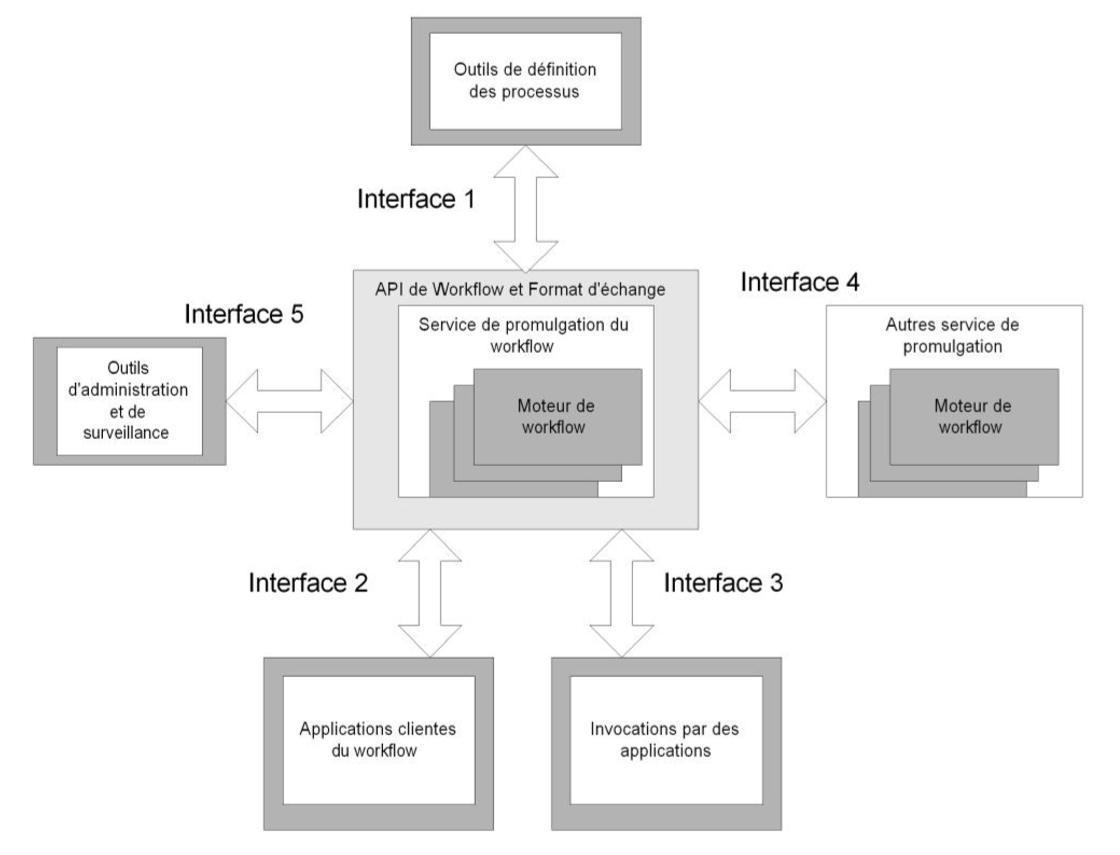
\includegraphics[width=1\linewidth]{Capture6}
	\caption{ Modèle de référence des systèmes de gestion de workflow (WfMC, 95). }
	\label{fig:capture6}
\end{figure}

\begin{itemize}
\item  \textbf{Interface 1} : Correspond à l’échange des modèles entre les moteurs de workflows et les différents outils de modélisation de processus.
\item  \textbf{Interface 2} : Permet à des applications clientes de communiquer avec le moteur de workflows. 
\item  \textbf{Interface3} : Permet au système de workflow d’invoquer des applications clientes. 
\item  \textbf{Interface 4} : Permet l’interopérabilité entre les différents moteurs de workflows. 
\item  \textbf{Interface 5} : Correspond à l’interaction entre les applications d’administration et de pilotage et le moteur de workflows.

\end{itemize}
\comment{

\subsubsection{Interface avec les Outils de définition de procédures }
Cette interface, située entre les outils de modélisation/définition et le logiciel de gestion
du Workflow pendant l’exécution, est nommée interface d’import/export de définition de processus. Cette interface définit le format d’échange et d’appels des APIs, qui permettent
l'échange d'informations de définition de procédures sur une variété de médias d'échange :
physiques ou électroniques. Cette interface permet l'échange d'une définition de processus
complète ou d’un sous-ensemble. Par exemple le changement de définition d’un ensemble de
procédures ou plus simplement la modification des attributs d'une activité particulière dans
une définition de procédures. 

\subsubsection{Interface avec les applications clientes Workflow }
La liste des tâches (Worklist) à exécuter par une ressource est généralement définie et gérée par le service d’exécution du Workflow. Cette liste doit pouvoir déclencher des appels à
des applications clientes diverses et des ressources. La solution retenue pour respecter la susdite exigence, consiste à encapsuler la variété d’application qui peut être utilisée derrière un jeu standard d'API le \ac{wapi}. Ce jeu permet ainsi d’utiliser une communication standardisée entre les applications clientes, le moteur de Workflow et les Worklist, indifféremment de la nature de l’implémentation réelle des produits
clients. 
\subsubsection{Interface avec les applications invoquées}
Il est évident que le système Workflow ne peut pas intégrer l’invocation automatique de
toutes les applications qu’il peut être amené à utiliser pendant l’exécution d’un Workflow. Par
exemple les applications dont les données sont fortement typées. Dans ce cas un composant
externe supplémentaire, nommé agent d’application, est ajouté, il est chargé de la traduction
des informations dans un format compréhensible par le standard WAPI. 

Dans le cas le plus simple, l'invocation d'application est traitée localement par un moteur
de Workflow, mais les applications invoquées peuvent être utilisées par plusieurs moteurs de
Workflow et peuvent se situer sur des machines distantes, il convient donc de définir un format commun d’utilisation des ces applications entre les Workflow dans le but de communiquer correctement et de synchroniser l’appel à ces applications. 

\subsubsection{Interface avec les autres Workflow }
Un des objectifs de la normalisation dans la définition de Workflow est de pouvoir
transmettre des WorkItem entre deux systèmes Workflow conçus par des concepteurs de systèmes Workflow différents. Trois principaux types d’interopérabilité ont étés identifiés : 

\textbf{Workflow chaînés :} La dernière activité d’un Workflow A doit pouvoir fournir un item à la première activité d’un Workflow B.

\textbf{ Workflow hiérarchiques :} une activité d’un Workflow A doit pouvoir être vu comme un
Workflow B. 

\textbf{Workflow Peer to Peer :} Une procédure globale est composée d’activités gérées en partie par un Workflow et en partie par un autre Workflow, sans système de supervision de
la procédure complète. 

\textbf{Workflow Synchronisés :} Deux Workflow s’exécutent en parallèle et doivent pouvoir se
synchroniser sur certaines activités. 

Pour résumer, il est possible d’identifier deux aspects principaux nécessaires à
l’inter fonctionnement de Workflow :

• L’interprétation commune de la définition de procédures (ou d’un sous-ensemble).

• L’appui pendant l'exécution de l’échange des divers types d'information de contrôle et
le transfert des données appropriées et/ou d'applications entre les services d’exécution Workflow différents.

\subsubsection{Interface avec les outils de contrôle et d’administration }


L’objectif de cette interface est de permettre à un logiciel de Monitoring de Workflow de
s’interfacer avec plusieurs Workflow différents et ainsi regrouper la supervision d’un ensemble de systèmes Workflow dans un logiciel.


L'interface 5 permet à une application de gestion indépendante d’interagir avec des
Workflow de différents domaines. L'application de gestion peut aussi se charger d'autres fonctions de gestion, au-delà de celles-ci. Par exemple, elle peut aussi gérer des définitions de procédures de Workflow, agissant comme un dépôt d’information commun à plusieurs systèmes
et distribuant des définitions de processus aux divers Workflow via des opérations au travers
de leurs interfaces 1.
Malgré cela, des scénarii d’implémentations moins modulaires sont aussi envisageables;
par exemple l'application de gestion peut être une partie intégrante du service d’exécution.  



}


% 
%
%
%
%\subsection{Comparaison entre types de workflows:} \ref{tab:tabl2}
% 
%\begin{center}
%\begin{table}[h]
%	\centering
%	
%	\begin{tabular}{| m{2cm} |m{8em}| m{8em} |m{6em}|m{7em}|}
%		\hline
%	\rowcolor[HTML]{38FFF8} 
%		\textbf{Critères} & \textbf{De production} & \textbf{Administratif} & \textbf{Ad-hoc} & \textbf{Collaboratif} \\ \hline
%		
%		\textbf{Capacité de traitement} &   Haute capacité de traitement Temps de réponse rapide.Le but est la Productivité & Capacité de traitement inferieure(10 à 100)fois moins que pour un workflow de production &  Facilite d'utilisation et d'apprentissage sont très importantes. &   Capacité de changer dynamiquement la définition d’un processus est essentielle \\ \hline
%		
%	\rowcolor[HTML]{96FFFB} 
%		\textbf{Utilisation} &  Employés travaillant à plein temps sur des activités  courtes. &  Un grand nombre d'employés peuvent être   impliqués & La modification dynamique et rapide des  processus est essentielle.  &  Fournir une voie structurée pour travailler ensemble  \\ \hline
%		
%		\textbf{ Nature des processus } & Processus formels avec peu de variation Les  processus peuvent  être trèscomplexes.&  Une variété de processus pout exister dans même système. Les processus peuvent être bien définis, mais  requièrent moins d'exigence.  & Facilité de  déploiement.&Les processus sont moins rigides \\ \hline
%		
%	\rowcolor[HTML]{96FFFB} 
%		\textbf{Spécificités} &  Requiert une intégration serrée avec les systèmes de bases. &  Utilise souvent des documents attaches.& Le but est de zéro coût  d’administration. &La capacité de traitement est de moindre importance
%		\\ \hline
%	\end{tabular}
%	
%	\caption{Comparaison entre types de Workflows.}
%	\label{tab:tabl2}
%\end{table}
%\end{center}
% 
% 
%\textbf{Exemples de workflows :}
%\begin{itemize}
%	\item Processus de déclaration de sinistre,
%	\item Processus d'ouverture compte,
%	\item Processus de création d'un dossier de prêt,
%	\item Processus de gestion d'une succession,
%	\item Processus de prise de congés.
%\end{itemize}







%\section{Architecture des systèmes de gestion de workflows }
%\subsection{Définition }
%La gestion du workflow est une technologie en évolution rapide, qui est de plus en plus exploitée par les entreprises. Un SGWf représente un système qui définit, implémente et gère l'exécution de workflows à l'aide d'un environnement logiciel fonctionnant avec un ou plusieurs moteurs de workflows et capable d'interpréter la définition d'un processus, de gérer la coordination des participants et d'invoquer des applications externes.  
%
% L'architecture de référence d’un SGWf proposée par la Workflow Management Coalition (WfMC, 95) en1995 est présentée dans la figure \ref{fig:capture6}. Ce modèle inclut un service de déploiement, qui contrôle l'exécution des workflows et qui supporte cinq interfaces standardisées:
% 
% 
% 
% 
% 
%\subsection{Standards utilisés dans les SGWf :}
%
%\begin{figure}[!h]
%	\centering
%	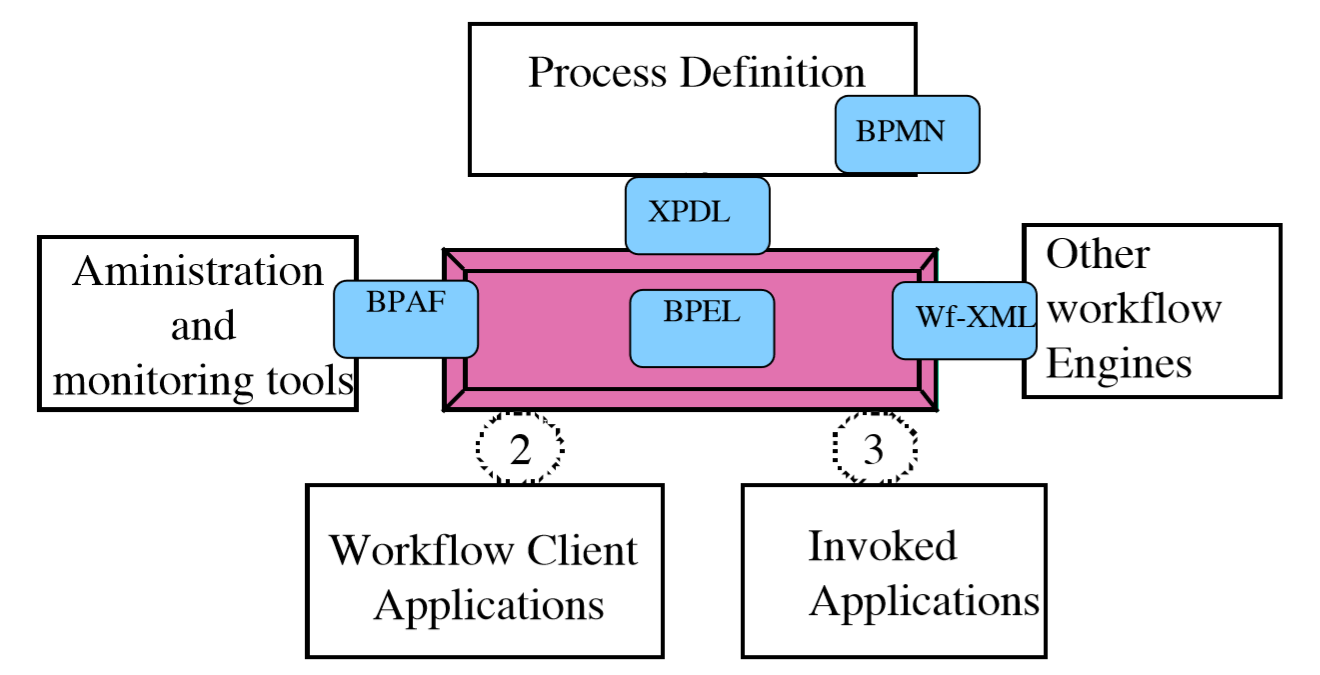
\includegraphics[width=0.7\linewidth]{Capture7}
%	\caption{Différents standards adoptés dans les SGWf}
%	\label{fig:capture7}
%\end{figure}
%
%
%\subsubsection {BPNM (Business Process Model and Notation)}
% est une représentation graphique permettant de spécifier les processus métier maintenus par le groupe de gestion d'objets (OMG). 
%\subsubsection {XPDL (Process Definition Language):} 
%est un format normalisé par la WfMC (Workflow Management Coalition) pour l’échange de définitions de partenaire entre différents produits de flux de travail, c.-à-d. entre différents outils de modélisation et suites de gestion. XPDL définit un schéma XML pour spécifier la partie déclarative du workflow / partenaire.
%\subsubsection {BPAF (Business Process Analytics)} 
%fournit aux participants aux processus et aux décideurs des informations sur l'efficacité des processus organisationnels.
%\subsubsection {BPEL (Business Process Execution Language)}
% BPEL est un langage d'orchestre.
%\subsubsection { Wf-XML }
%est un standard BPM développé par la Workflow Management Coalition. Wf-XML offre à un moteur BPM un moyen standard d'appeler un processus dans un autre moteur BPM et d'attendre qu'il se termine.
% 
 

\section{ Intérêt du cloud pour les workflows }
Les clouds offrent plusieurs avantages pour les applications à base de workflows. 
Ces avantages facilitent: 
\subsection{L’approvisionnement de ressources }
Dans les grilles, l'ordonnancement est basé sur un modèle en best-effort, dans lequel l’utilisateur spécifie la quantité de temps nécessaire et délègue la responsabilité de l'allocation des ressources et d'ordonnancement de tâches à un ordonnanceur fonctionnant en mode batch utilisant des files d’attentes. Dans le cloud, au lieu de déléguer l’allocation au gestionnaire de ressources, l'utilisateur peut provisionner les ressources nécessaires et ordonnancer les tâches en utilisant un ordonnanceur contrôlé par l'utilisateur. Ce modèle d’approvisionnement est idéal pour les workflows, car il permet au système de gestion de workflow d'allouer une ressource une seule fois et de l'utiliser pour exécuter de nombreuses tâches. 
\subsection{L’allocation dynamique de ressources à la demande }
Contrairement aux grilles, les clouds donnent l'illusion que les ressources informatiques disponibles sont illimitées. Cela signifie que les utilisateurs peuvent demander, et s’attendre à obtenir des ressources suffisantes pour leurs besoins, à tout moment. L’approvisionnement à la demande est idéal pour les workflows et d'autres applications faiblement couplées, car il réduit le surcoût (overheads) d’ordonnancement total et peut améliorer considérablement les performances du workflow (Singh, 2005 ; Juve, 2008) 
\subsection{L’élasticité}
Outre l’approvisionnement des ressources à la demande, les clouds permettent aussi aux utilisateurs de libérer des ressources à la demande. La nature élastique de clouds facilite le changement des quantités et des caractéristiques de ressources lors de l'exécution, permettant ainsi d’augmenter le nombre de ressources, quand il y a un grand besoin, et d’en diminuer, lorsque la demande est faible. Cela permet aux systèmes de gestion de workflow de répondre facilement aux exigences de qualité de service (QoS) des applications, contrairement à l'approche traditionnelle, qui nécessite de réserver à l'avance des ressources dans les environnements de grilles. 
\subsection{La garantie des QoS via des SLA }
Avec l’arrivée des services de cloud computing  provenant de grandes organisations commerciales, les accords de niveau de service (SLA) ont été une préoccupation importante pour les fournisseurs et les utilisateurs. En raison de compétitions entres les fournisseurs de services émergents, un grand soin est pris lors de la conception du SLA qui vise à offrir (i) de meilleures garanties de QoS aux utilisateurs, et (ii) des termes clairs pour l'indemnisation, en cas de violation du contrat. Cela permet aux systèmes de gestion de workflow de fournir de meilleures garanties de bout en bout en "mappant" les utilisateurs aux fournisseurs de services selon les caractéristiques des SLA.

\subsection{Le faible Coût d’exploitation }
 Économiquement motivés, les fournisseurs de cloud commercial s'efforcent d'offrir de meilleures garanties de services par rapport aux fournisseurs de grille. Les fournisseurs de cloud profitent également des économies d'échelle, en fournissant des ressources de calcul, de stockage et de bande passante, à un coût très faible grâce, à la virtualisation. Ainsi l'utilisation des services de cloud public pourrait être économique et une alternative moins coûteuse, par rapport à l’utilisation de ressources dédiées, qui sont plus chères. Un des avantages de l'utilisation des ressources virtuelles pour l'exécution de workflow, plutôt que d'un accès direct à la machine physique, est le besoin réduit pour sécuriser les ressources physiques des codes malveillants. Cependant, l'effet à long terme de l'utilisation de ressources virtuelles dans les clouds qui partagent efficacement une "tranche" de la machine physique, plutôt que d'utiliser des ressources dédiées pour les workflows de calculs intensifs, est une question de recherche intéressante.
 %
 %
 %
 %
 %
 %
 %%%%%%%%%%%%%%%%%%%%%%%%%%%%%%%%%%%%%%%%%%%%%%%%%%%%%%%%%%%%%%%%%%%%%%%%%%%%%%%%%%%%
 \comment{
 	\section{Modélisation des processus workflow
 	}
 	La modélisation est une activité qui précède toute décision ou formulation, elle permet de représenter la description du système réel. Tout comme un système informatique, le système workflow comporte un certain nombre d'aspects à modéliser. Nous présentons en premier lieu ces aspects, nous décrivons en second lieu les principales techniques de modélisation utilisées dans le domaine de workflow et nous terminons cette section par évoquer certains aspects temporels et organisationnels des workflows.
 	
 	\subsection{Aspects à modéliser}
 	\subsubsection{L'aspect fonctionnel}
 	L'aspect fonctionnel concerne l'identification des activités des processus que l'on souhaite modéliser. Il est important de comprendre qu'il ne s'agit pas uniquement d'identifier les fonctions des différents départements d'une organisation mais aussi de distinguer les activités composant un processus. La modélisation fonctionnelle doit également permettre d'établir la hiérarchie des activités, i.e. d'exprimer de possibles décompositions en termes de sous-processus. 
 	
 	Enfin, le modèle fonctionnel doit aussi représenter le flux de données associées aux activités et les interdépendances de données entre les activités (data flow). 
 	\subsubsection{L'aspect comportemental}
 	L'aspect comportemental est un aspect primordial du workflow puisqu'il correspond à la dynamique du processus. Le comportement s'exprime par la modélisation d'un contrôle de flux entre les activités. Ce dernier permet d'indiquer la chronologie de l'exécution des activités, leur flux (séquentiel ou parallèle), les points de synchronisation entre activités ou au contraire, les points de disjonction. De plus, le modèle comportemental doit représenter les événements qui permettent de déclencher les activités. Nous soulignons l'importance de ce modèle, qui permet l'exécution du workflow. L'aspect comportemental est également appelé aspect de coordination.
 	\subsubsection{ L'aspect informationnel (données) }
 	Cet aspect concerne l'ensemble des informations et des données qui sont associées
 	aux activités. Le modèle informationnel, souvent négligé lors de l'implémentation d'un workflow \parencite{Geelan}arencite{Geelan}arencite{b3}, décrit en détail les relations qui existent entre les données, leur type et leur structure.
 	\subsubsection{L'aspect organisationnel }
 	Comme son nom l'indique, la partie organisationnelle concerne la description de l'organisation des acteurs de l'entreprise. Le modèle organisationnel peut soit refléter fidèlement l'organigramme de l'entreprise, c'est à dire la décomposition hiérarchique de celle-ci en départements et services soit décrire des unités organisationnelles dans lesquelles on identifie des acteurs. Selon la méthode choisie, la description est plus ou moins détaillée et permet d'établir des liens hiérarchiques entre les acteurs ainsi que des relations entre unités organisationnelles ou départements. Toutefois, quelle que soit la méthode retenue, la description des rôles associés aux différentes activités reste invariante. Les rôles créent l'interface entre le modèle organisationnel et les modèles représentant les activités.
 	
 	
 	
 	\subsection{Modélisation de Workflow adaptable }
 	
 	Dans le cas particulier de la modélisation des Workflow adaptables, plusieurs approches sont proposées \parencite{Han}. 
 	
 	\subsubsection{ Approche Meta modèle}
 	Cette approche emploie un méta modèle pour déterminer la structure et les types de composants constitutifs; elle définit un jeu de primitives pour transformer un modèle Workflow générique ou une instance de modèle. 
 	
 	\subsubsection{ L’approche de point ouvert Open-point }
 	Elle définit des points spéciaux dans un modèle de Workflow, où l’adaptation peut être faite. Cette approche inclut la mise à disposition de choix multiples pour les utilisateurs, l’allocation dynamique de certaines ressources aux tâches en run time, ou une interface ouverte par laquelle une « dernière modélisation » peut être réalisée. La « dernière modélisation » signifie que, pendant l’exécution des modèles complets, certains sous modèles peuvent être définis dynamiquement pour une utilisation immédiate. 
 	\subsubsection{ Approche synthétisée}
 	Il semble que les deux approches puissent être employées complémentairement pour la définition de Workflow adaptable. Pour cela, les deux hypothèses suivantes doivent être prises en compte :
 	
 	Tout d’abord, il parait nécessaire de distinguer les évolutions de procédures Workflow et les changements ad hoc dynamique dans une procédure. De plus, une séparation claire est faite entre le build time et le run time en termes de Workflow. Il parait impératif de faciliter le franchissement bilatéral de cette frontière pour rendre modélisables les Workflow adaptables.
 	
 	En synthèse, il est souhaitable de définir la frontière entre les changements ad hoc et les évolutions du Workflow. Il semblerait que ces changements devraient être testés sur une instance de modèles puis si nécessaires propagés au niveau global pour une modification persistante.
 } 
%%%%%%%%%%%%%%%%%%%%%%%%%%%%%%%%%%%%%%%%%%%%%%%%%%%%%%%%%%%%%%%%%%%%%%%%%%%%%%%%%%%%
  \section{Modélisation de workflow avec les réseaux de pétri}

Les Réseaux de Petri (RdPs)  constituent un formalisme majeur pour modéliser les processus workflows. Une des forces des RdPs est la base mathématique forte qu'ils offrent avec une représentation graphique. 


%%%%%%%%%%%%%%%%%%%%%%%%%%%%%%%%%%%%%%%%%%%%%%%%%%%%%%%%%%%%%%%%%%%%%%
\section{les réseaux de Pétri}



\subsection{Qu'est-ce que les réseaux de Pétri }
Les réseaux de Pétri sont définis comme étant un formalisme qui permet la description et l'analyse du comportement des systèmes concurrents, introduit par Carl Adam Pétri en 1962. \parencite{Rdp}



\begin{defn}\textbf{\textbf{(Définition d'un réseau de pétri:)}}
	\\
	Un réseau de pétri (R) est un triple R= (P, T, W) où P est l'ensemble des places (les places représentent les sites) et T l'ensemble des transitions (les transitions représentent les actions) tel que :
	
	\begin{itemize}
		\item  	P est un ensemble final de places,
		\item T est un ensemble final de transition $ (P \cap T = \theta ) $, 
		\item W: $(P \times T) \cup (T \times P)\to N = \{0,1,2,...\} $.  
	\end{itemize}
	
\end{defn}








\subsection{Représentation d'un réseau de Pétri }



\subsubsection{Représentation graphique} 
L'un des aspects les plus agréables des réseaux de Pétri est qu'il est extrêmement aisé de les visualiser; c.-à-d., donner une interprétation graphique à sa structure qui peut être représentée à travers un graphe bipartie fait de deux types de sommets: les places et les transitions reliées alternativement par des arcs orientés qui portent des poids entiers positifs, si un poids n'est pas porté alors il est égal à 1 (RdP ordinaire). Généralement, les places sont représentées par des cercles et les transitions par des rectangles, le marquage d'un RdP est représenté par la distribution de jetons dans l'ensemble de ses places telle que chaque place peut contenir un ou plusieurs jetons représentés par des points dans le cercle représentant la place. \parencite{belounnar2011approche}



\begin{figure}[h]
	\centering
	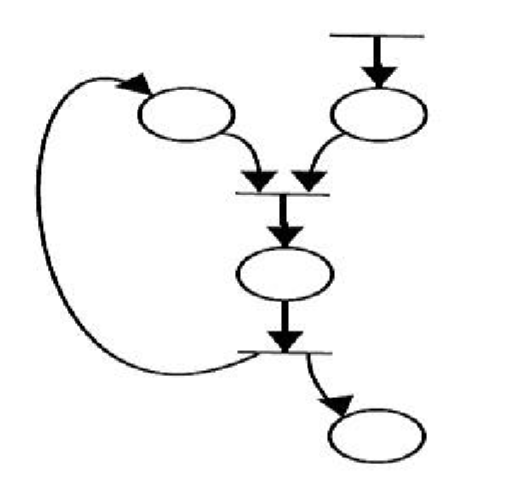
\includegraphics[width=0.5\linewidth]{images/petrif01}
	\caption{ Réseau de Pétri simple }
	\label{fig:petrif01}
\end{figure}
\subsubsection{ Représentation matricielle} 
Une représentation matricielle d'un RdP est offerte afin de simplifier les Tâches d'analyse et de vérification effectuée sur un modèle RdP. Agir sur une représentation graphique d'un modèle RdP est une Tâche délicate en comparant avec une représentation matricielle. Il   est possible de représenter la fonction W (fonction de poids) par des matrices.\parencite{Rdp}

\begin{defn}\textbf{\textbf{(Réseau de pétri):}}
	Soit Un réseau de pétri $ R= (P, T, W) $ avec $ P= \{p1, p2, …, pm\} $ et $ T= \{t1, t2, …,tn \}$, on appelle matrice des pré conditions   pré la matrice  $  m \times n $   à coefficients dans  N  tel que $ pre (i,j)= W(p_{i}, t_{j}) $,  elle indique le nombre de marques que doit contenir la place $p_{i}$ pour que la transition $ tj $  devienne franchissable, de la même manière on définit la matrice des post conditions post  la matrice $ n  \times m $ tel que $ post (i,j)= W(tj,  p_{i}) $ contient le nombre de   marques déposées dans $p_{i}$ lors du franchissement de la transition $t_{j}$. La matrice C= post – pré est appelée matrice d'incidence du réseau (m représente le nombre de places d'un réseau de Pétri et n le nombre de transitions.). 
\end{defn}

La représentation Graphique d’un marquage dans un RdP marqué est présentée par des marques dans la place appelées jetons. 

Le marquage d'un réseau de Petri est représenté par un vecteur de dimension m à coefficients dans N. La règle de franchissement d'un réseau de Petri est définie par :    $     M’ (p) =M (p) +  C (p, t).  $



\subsubsection{Représentation d’un RdP marqué }

Un réseau de Pétri marqué est le couple $ N = < R , M > $ où : 
\begin{itemize}
	\item R est un réseau de Pétri. 
	\item M est une application de marquage.  
	\item $  M : P \to N  $. 
\end{itemize}


$ M(p) $ est le nombre de marques (jetons) contenus dans la place p. Le marquage d’un réseau de Pétri est une opération qui consiste à assigner des jetons dans les places.

On appelle marquage M d’un Réseau de Pétri le vecteur du nombre de marques dans chaque place : la $ I^{eme} $ composante  correspond au nombre de marques dans la $ I^{eme} $   place. Il indique à un instant donné l'état du RdP.\parencite{Rdp}   


\begin{exmp}
	
	
	\begin{figure}[H]
		\centering
		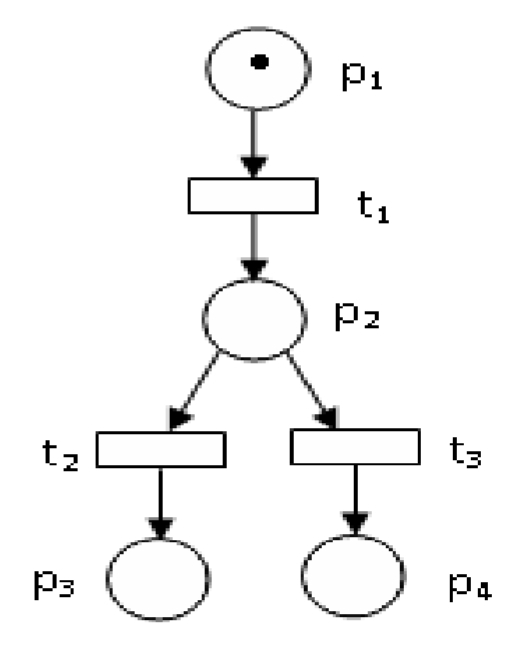
\includegraphics[width=0.4\linewidth]{images/pitref02PNG}
		\caption{ Réseau de Pétri marqué }
		\label{fig:pitref02png}
	\end{figure}
	
	Pour le réseau de la (Figure \ref{fig:pitref02png}). 
	
	$ P= \{p1, p2, p3, p4\}$ et $T= \{t1, t2, t3\}  $
	
	
	\begin{figure}[H]
		\centering
		
		\begin{subfigure}[b]{0.4\textwidth}
			\[
			pre=
			\begin{pmatrix}
			1 & 0 & 0 \\
			0 & 1 & 1 \\
			0 & 0 & 0 \\
			0 & 0 & 0
			\end{pmatrix}
			\]
			\caption{La matrice pré}
		\end{subfigure}
		\hfill
		\begin{subfigure}[b]{0.4\textwidth}
			\[	post=
			\begin{pmatrix}
			0 & 0 & 0 \\
			1 & 0 & 0 \\
			0 & 1 & 0 \\
			0 & 0 & 1 
			\end{pmatrix}
			\]
			\caption{La matrice post}
		\end{subfigure}
		
		
		
		\begin{subfigure}[b]{0.4\textwidth}
			\[
			C=
			\begin{pmatrix}
			-1 & 0 & 0 \\
			1 & -1 & -1 \\
			0 & 1 & 0 \\
			0 & 0 & 1
			\end{pmatrix}
			\]
			\caption{La matrice d'incidence}
		\end{subfigure}
		\hfill
		\begin{subfigure}[b]{0.4\textwidth}
			\[	M=
			\begin{pmatrix}
			1  \\
			0  \\
			0  \\
			0 
			\end{pmatrix}
			\]
			\caption{Le vecteur de marquage M }
		\end{subfigure}
		
	\end{figure}
	
	Le marquage du RdP présenté à la Figure 3 est donné par : 
	\[	M=
	\begin{pmatrix}
	1  \\
	0  \\
	0  \\
	0 
	\end{pmatrix}
	\]
	On appelle marquage initial, noté M0, le marquage à l’ instant initial (t = 0). 
\end{exmp}



\subsection{réseaux workflow (Wf-nets)}
\begin{defn}
	\textbf{(Wf-nets):}  Le réseau de pétri qui permet de modéliser le contrôle de flux d’un workflow est appelé un WF-net  (réseaux workflow) Ssi:\parencite{sbai2010contribution}
	
	\begin{enumerate}
		\item Il existe une seule place source $i \in P$ avec $ ^{*}i = \emptyset $.  (i début du processus).
		
		\item  Il existe une seule place puits $o \in P$ avec $ ^{*}o = \emptyset $  (o est la fin du processus).
		
		\item  Chaque nœud $x \in (P \cup T) $est sur un chemin de $i$ à $o$. C’est à dire : Chemin $(i, x)$ $\wedge$ Chemin $(x, o)$.
		
		
		
	\end{enumerate} 
	
	\begin{figure}[H]
		\centering
		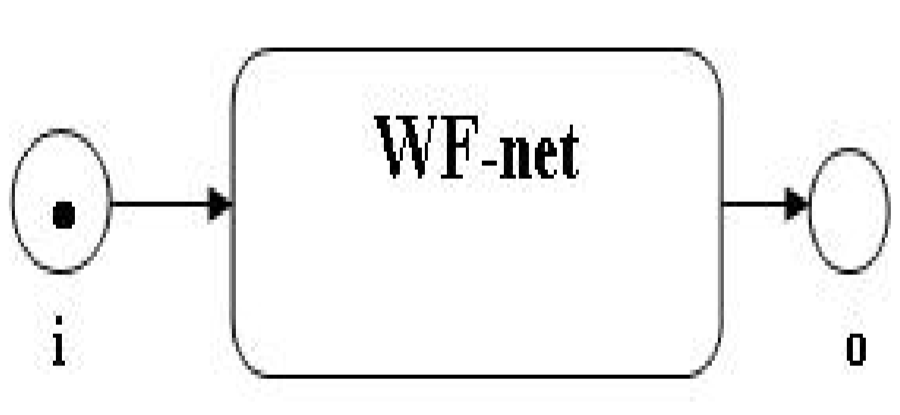
\includegraphics[width=0.5\linewidth]{images/wf-nete006}
		\caption{ Procédure modélisée avec le WF-net }
		\label{fig:wf-nete006}
	\end{figure}
	
\end{defn}
Un réseau de workflow (WF-net) est un réseau de pétri qui possède une seule place d’entrée (i) et une seule place de sortie (o) et puis que n’importe quel cas traité avec la procédure représentée par un WF-net est crée au moment de début de son traitement par le système de gestion de workflow (SGWF) est supprimé une fois que sont traitement est complètement achevé par le SGWF. Cela veut dure que le WFnet spécifie le cycle de vie d’un cas du processus modélisé.  \parencite{sbai2010contribution}
\begin{rem}
	Un chemin C dans un WF-net d’un nœud $n_{1}$ au nœud $n_{k}$ est une séquence $<n_{1},n_{2},...,n_{k}>$ tel-que $<n_{i},n_{i+1}> \in F $, pour $i=1...k-1$.
	F est la relation de flux. 
\end{rem}

\subsection{Constructions du routage dans un WF-net}
Un réseau de workflow (WF-net) est utilisé pour spécifier le routage de flux dans les cas du workflow, quatre types de routage ont été identifiés :\parencite{sbai2010contribution}

\subsubsection{Séquentiel :}

Utilisé pour traiter la relation de causalité entre les tâches. Soit deux tâches A et B, si la tâche B et exécutée après l’accomplissement de A, ce comportement peut être modélisé avec un RDP en ajoutant les places pour capter les relations de causalité entre les tâches A et B. La figure \ref{fig:wf003} illustre ce comportement.


\begin{figure}[H]
	\centering
	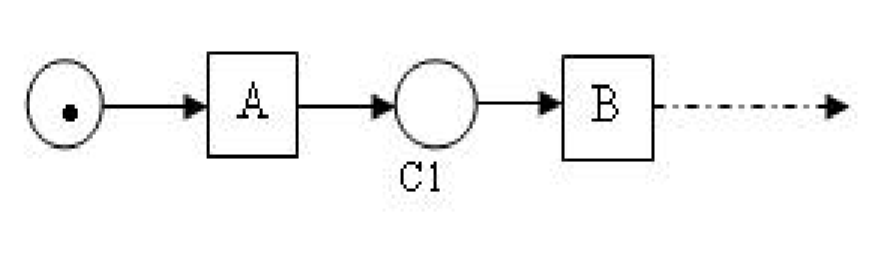
\includegraphics[width=0.7\linewidth]{images/wf003}
	\caption{Routage séquentiel.}
	\label{fig:wf003}
\end{figure}

\subsubsection{Parallèle : }
Utiliser dans le cas où l’ordre d’exécution est moins strict. Par exemple si on a deux tâches B et C qui doivent être exécutées mais dans un ordre arbitraire, la modélisation de ce comportement de routage parallèle comporte deux constructions le AND-split et AND-join.


\begin{figure}[H]
	\centering
	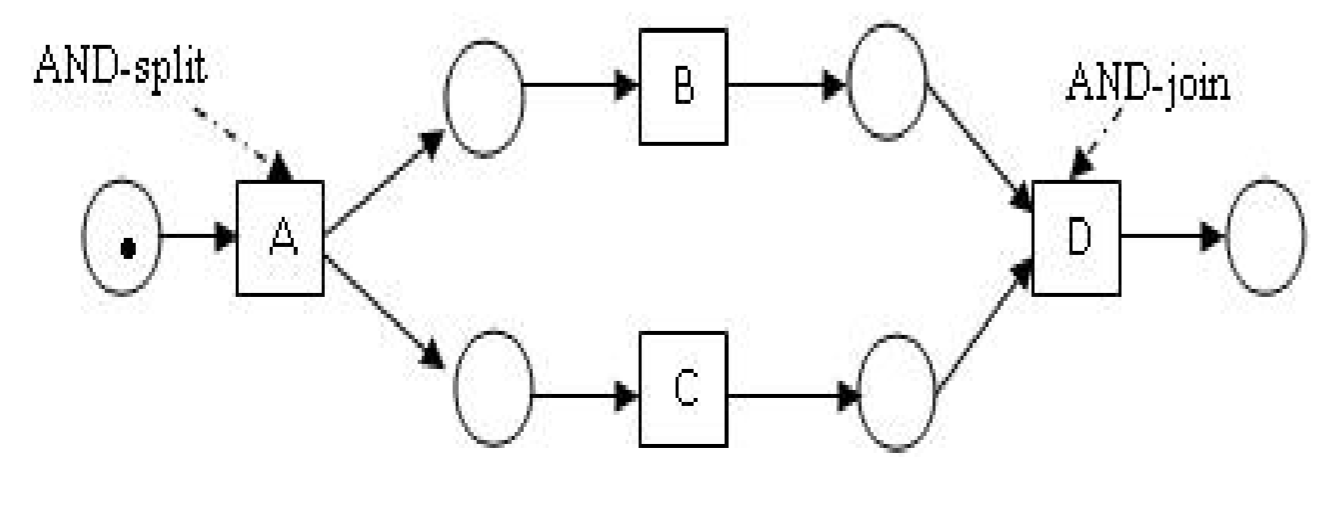
\includegraphics[width=0.7\linewidth]{images/Capture}
	\caption{Routage parallèle.}
	\label{fig:capture}
\end{figure}

\subsubsection{Conditionnel :}

Utilisé pour traiter les cas où le routage de flux peut dépendre des données d’un cas. Il existe deux types de routage conditionnel : \textit{\textbf{le choix non-déterministe}} et \textit{\textbf{le choix déterministe}}. 


\begin{enumerate}
	
	\item \textbf{Choix non-déterministe :} Pour modéliser ce comportement deux constructions sont utilisées OR-Split et OR-join. La figure \ref{fig:wf005} représente un choix entre l’exécution des deux tâches B ou C grâce à un jeton dans la place c2, mais cela permet un choix non-déterministe (l’exécution de B ou de C car les deux tâches sont permises).
	
	
	
	\begin{figure}[H]
		\centering
		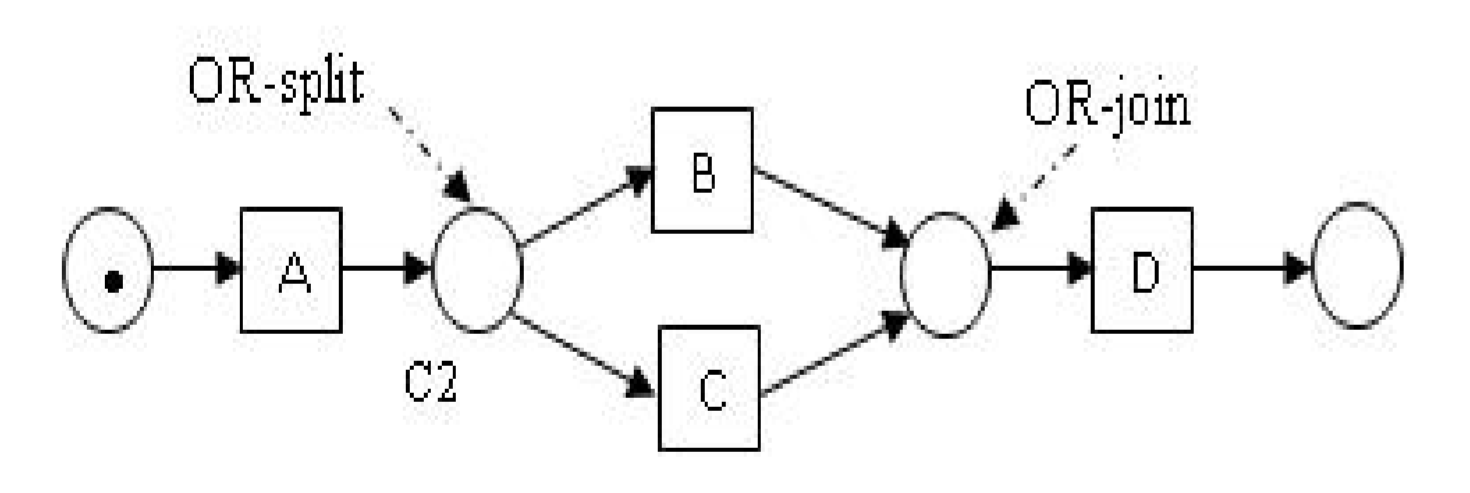
\includegraphics[width=0.7\linewidth]{images/wf005}
		\caption{Routage conditionnel non-déterministe}
		\label{fig:wf005}
	\end{figure}
	
	
	
	\item \textbf{Choix déterministe : } Le choix entre plusieurs alternatives peut être guidé par les données (ou les attributs) du workflow, dans ce cas c’est un choix déterministe.
	
	Nous pouvons prendre le schéma de la figure précédente et ajouter une pré-condition pour chacune des tâches B et C (en se basant sur un ou plusieurs attributs du workflow).
	
	Il y a une autre façon de modéliser le choix déterministe comme dans la figure suivante. La transition A comporte deux places de sortie c2 et c3 et produit un seul jeton (soit dans c2 ou dans c3). Le choix entre les deux places est basé sur la valeur de l’attribut x. Un symbole spécial est utilisé pour représenté que la tâche A est un OR-split (exclusive OR).
	
	
	\begin{figure}[H]
		\centering
		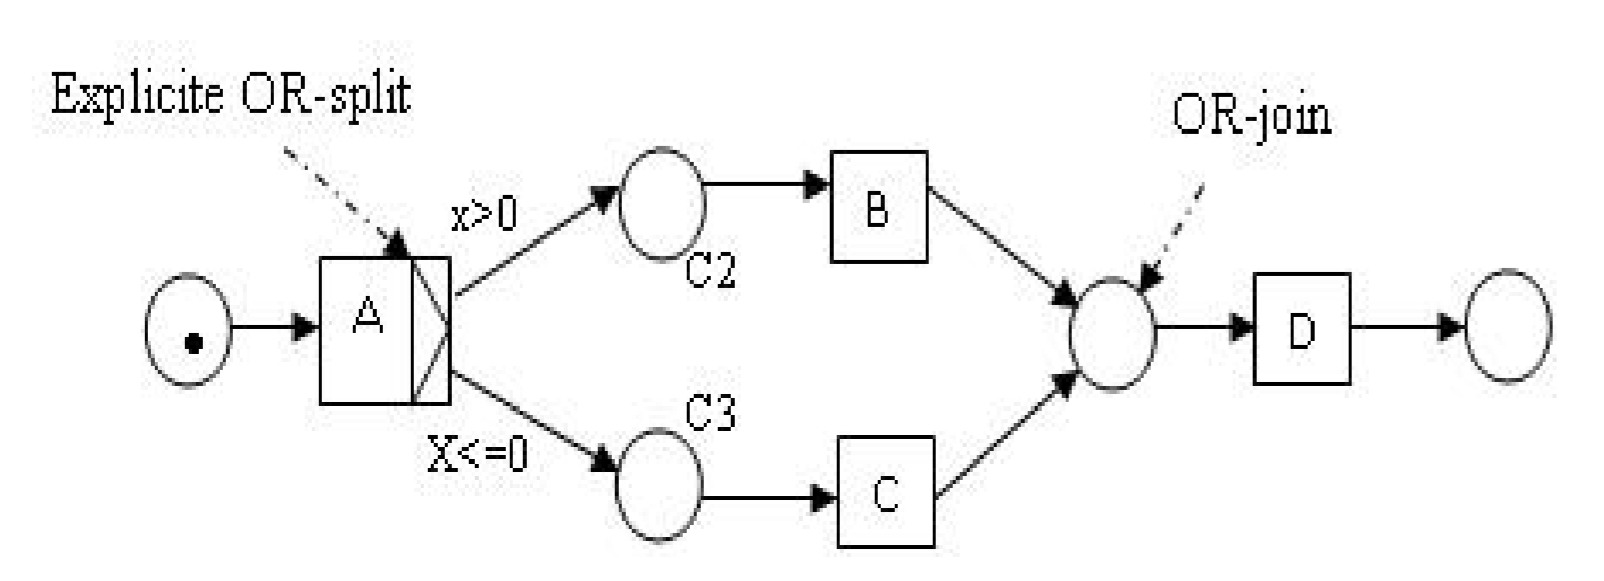
\includegraphics[width=0.7\linewidth]{images/wf006}
		\caption{Choix explicite entre B et C à base de l’attribut x. 
		}
		\label{fig:wf006}
	\end{figure}
	

\end{enumerate}

\subsubsection{Itération :} L’itération peut être modélisée en utilisant l’implicite (OR-split, OR-join), l’explicite (OR-split, OR-join). Il est utilisé dans le cas où une ou plusieurs tâches peuvent être exécutées plusieurs fois. La figure suivante montre un exemple d’un modèle de workflow en utilisant un routage itératif.


\begin{figure}[H]
	\centering
	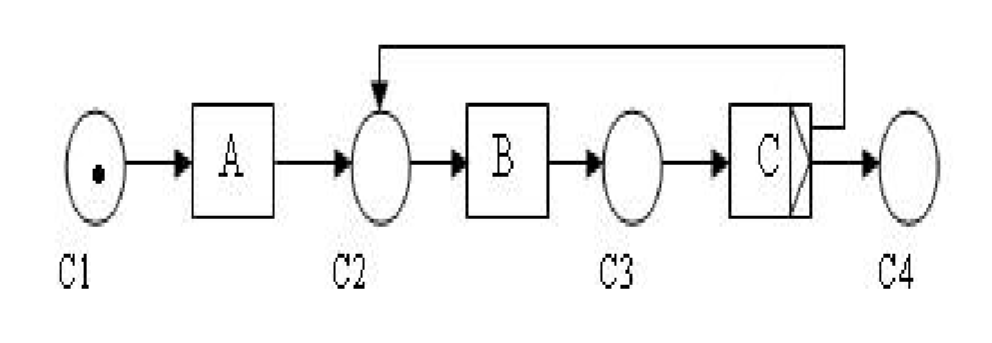
\includegraphics[width=0.7\linewidth]{images/wf008}
	\caption{Itération : B peut être exécutée plusieurs fois}
	\label{fig:wf008}
\end{figure}



\section{Conclusion}
Dans ce chapitre, nous avons étudié la théorie sur les concepts fondamentaux de cloud et de workflow. 

Dans le chapitre suivant, nous expliquerons l'étape d'analyse et la conception du système de flux de travail administratif, en prenant en compte l'étude théorique.

\chapter{Modélisations et Réseau de Petri}
 	 \section*{Introduction}
 	  
    Les Réseau de Pétri représentent un outil mathématique puisant dans le domaine de la modélisation et de la vérification des systèmes. En plus de leur force d’analyse, ils offrent une représentation graphique simple qui aide à la modélisation des systèmes complexes. 
    
    Donc Le modèle des réseaux de Pétri est un outil graphique de modélisation et d'analyse des systèmes parfaitement adapté à l'étude des structures de contrôle. Il permet notamment de maîtriser et d'assurer la sûreté de fonctionnement de logiciels complexes (aéronautique, transports, industrie...). 
    
    Le formalisme formel des Réseau de Pétri (RdP), adapté à la prise en compte des problèmes de concurrence, de synchronisme et de parallélisme, constitue un excellent outil de spécification fonctionnelle d'un problème et de mise en évidence des contraintes. Les propriétés mathématiques qui découlent de l'analyse des RdPs permettent une étude comportementale et structurelle essentielle à la validation d'une spécification. Les possibilités de simulation offertes par les outils informatiques supportant le formalisme contribuent également à cette validation. 
    
    En général, les méthodes de l'étude de systèmes par réseau de pétri se composent de trois étapes : premièrement on écrit le système en termes de réseau, pour obtenir un modèle en réseau ; deuxièmement on analyse le modèle obtenu, pour en déduire des propriétés comme l’absence de blocage, existence d'une solution, etc. Finalement, on fait la révision des propriétés obtenues pour montrer si le système est bon. Le résultat de cette méthode nous indique une analyse qualitative du système. Elle constitue une approche très importante pour avoir une bonne évaluation des systèmes.
    
    
 %La modélisation par les processus dont les domaines d'application étaient relativement restreints à l'origine, n'a cessé de progresser. Elle s'impose, aujourd'hui, en tant qu'outil incontournable, placé au cœur de la gestion des organisations. La déclinaison des processus organisationnels au niveau des architectures logicielles a donné, entre autres, naissance au workflow afin de répondre à des besoins divers dont celui d'optimisation des processus opérationnels, support et de pilotage.
%
%\section{Modélisation des processus workflow
%}
%La modélisation est une activité qui précède toute décision ou formulation, elle permet de représenter la description du système réel. Tout comme un système informatique, le système workflow comporte un certain nombre d'aspects à modéliser. Nous présentons en premier lieu ces aspects, nous décrivons en second lieu les principales techniques de modélisation utilisées dans le domaine de workflow et nous terminons cette section par évoquer certains aspects temporels et organisationnels des workflows.
%
%\subsection{Aspects à modéliser}
%\subsubsection{L'aspect fonctionnel}
%L'aspect fonctionnel concerne l'identification des activités des processus que l'on souhaite modéliser. Il est important de comprendre qu'il ne s'agit pas uniquement d'identifier les fonctions des différents départements d'une organisation mais aussi de distinguer les activités composant un processus. La modélisation fonctionnelle doit également permettre d'établir la hiérarchie des activités, i.e. d'exprimer de possibles décompositions en termes de sous-processus. 
%
%Enfin, le modèle fonctionnel doit aussi représenter le flux de données associées aux activités et les interdépendances de données entre les activités (data flow). 
%\subsubsection{L'aspect comportemental}
%L'aspect comportemental est un aspect primordial du workflow puisqu'il correspond à la dynamique du processus. Le comportement s'exprime par la modélisation d'un contrôle de flux entre les activités. Ce dernier permet d'indiquer la chronologie de l'exécution des activités, leur flux (séquentiel ou parallèle), les points de synchronisation entre activités ou au contraire, les points de disjonction. De plus, le modèle comportemental doit représenter les événements qui permettent de déclencher les activités. Nous soulignons l'importance de ce modèle, qui permet l'exécution du workflow. L'aspect comportemental est également appelé aspect de coordination.
%\subsubsection{ L'aspect informationnel (données) }
%Cet aspect concerne l'ensemble des informations et des données qui sont associées
%aux activités. Le modèle informationnel, souvent négligé lors de l'implémentation d'un workflow \parencite{b3}, décrit en détail les relations qui existent entre les données, leur type et leur structure.
%\subsubsection{L'aspect organisationnel }
%Comme son nom l'indique, la partie organisationnelle concerne la description de l'organisation des acteurs de l'entreprise. Le modèle organisationnel peut soit refléter fidèlement l'organigramme de l'entreprise, c'est à dire la décomposition hiérarchique de celle-ci en départements et services soit décrire des unités organisationnelles dans lesquelles on identifie des acteurs. Selon la méthode choisie, la description est plus ou moins détaillée et permet d'établir des liens hiérarchiques entre les acteurs ainsi que des relations entre unités organisationnelles ou départements. Toutefois, quelle que soit la méthode retenue, la description des rôles associés aux différentes activités reste invariante. Les rôles créent l'interface entre le modèle organisationnel et les modèles représentant les activités.
%
%
%
%\subsection{Modélisation de Workflow adaptable }
%
%Dans le cas particulier de la modélisation des Workflow adaptables, plusieurs approches sont proposées [HAN 98]. 
%
%\subsubsection{ Approche Meta modèle}
%Cette approche emploie un méta modèle pour déterminer la structure et les types de composants constitutifs; elle définit un jeu de primitives pour transformer un modèle Workflow générique ou une instance de modèle. 
%
%\subsubsection{ L’approche de point ouvert Open-point }
%Elle définit des points spéciaux dans un modèle de Workflow, où l’adaptation peut être faite. Cette approche inclut la mise à disposition de choix multiples pour les utilisateurs, l’allocation dynamique de certaines ressources aux tâches en run time, ou une interface ouverte par laquelle une « dernière modélisation » peut être réalisée. La « dernière modélisation » signifie que, pendant l’exécution des modèles complets, certains sous modèles peuvent être définis dynamiquement pour une utilisation immédiate. 
%\subsubsection{ Approche synthétisée}
%Il semble que les deux approches puissent être employées complémentairement pour la définition de Workflow adaptable. Pour cela, les deux hypothèses suivantes doivent être prises en compte :
%
%Tout d’abord, il parait nécessaire de distinguer les évolutions de procédures Workflow et les changements ad hoc dynamique dans une procédure. De plus, une séparation claire est faite entre le build time et le run time en termes de Workflow. Il parait impératif de faciliter le franchissement bilatéral de cette frontière pour rendre modélisables les Workflow adaptables.
%
%En synthèse, il est souhaitable de définir la frontière entre les changements ad hoc et les évolutions du Workflow. Il semblerait que ces changements devraient être testés sur une instance de modèles puis si nécessaires propagés au niveau global pour une modification persistante.


\section{Réseau de Pétri}

\subsection{Qu'est-ce que les réseaux de Pétri }
Les réseaux de Pétri sont définis comme étant un formalisme qui permet la description et l'analyse du comportement des systèmes concurrents, introduit par Carl Adam Pétri en 1962. [1]  Les définitions concernant les réseaux de Pétri portaient sur deux aspects :


\begin{itemize}
	\item \textbf{	Un aspect structurel }
\\
	Quelles sont les actions, quels sont les sites, quelles sont les conditions pour qu'une action soit possible et quelles sont les conséquences d'une action?
	
	\item \textbf{ Un aspect comportemental}
	\\
	Comment représenter le fonctionnement d'un réseau de Pétri? C.-à-d. ce qui se passe quand une action ou plusieurs actions sont exécutées.
\end{itemize}

\subsection{L'aspect structurel}
\begin{defn}\textbf{\textbf{(Définition d'un réseau de pétri:}}
	\\
Un réseau de pétri (R) est un triple R= (P, T, W) où P est l'ensemble des places (les places représentent les sites) et T l'ensemble des transitions (les transitions représentent les actions) tel que :
	
	\begin{itemize}
		\item  	P est un ensemble final de places,
		\item T est un ensemble final de transition $ (P \cap T = \theta ) $ ,
		\item W: $(P \times T) \cup (T \times P)\to N = \{0,1,2,...\} $  .
	\end{itemize}
	
\end{defn}

\subsubsection{Représentation d'un réseau de Pétri }


 
 \subsubsection*{Représentation graphique} 
  L'un des aspects les plus agréables des réseaux de Pétri est qu'il est extrêmement aisé de les visualiser; c.-à-d., donner une interprétation graphique à sa structure qui peut être représentée à travers un graphe bipartie fait de deux types de sommets: les places et les transitions reliées alternativement par des arcs orientés qui portent des poids entiers positifs, si un poids n'est pas porté alors il est égal à 1 (RdP ordinaire). Généralement, les places sont représentées par des cercles et les transitions par des rectangles, le marquage d'un RdP est représenté par la distribution de jetons dans l'ensemble de ses places telle que chaque place peut contenir un ou plusieurs jetons représentés par des points dans le cercle représentant la place. [2]
 
 
 
\begin{figure}[h]
	\centering
	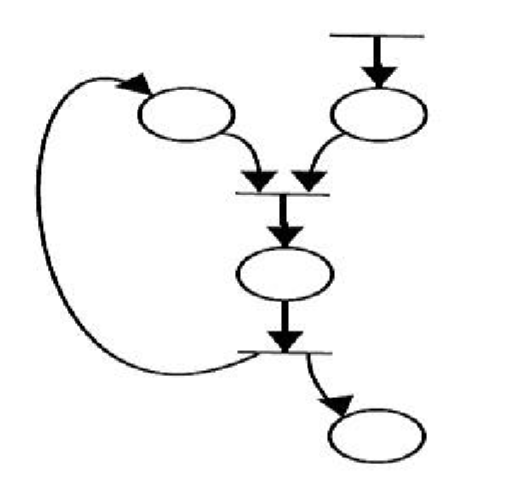
\includegraphics[width=0.5\linewidth]{images/petrif01}
	\caption{ Réseau de Pétri simple }
	\label{fig:petrif01}
\end{figure}
 	 \subsubsection*{ Représentation matricielle} 
 	Une représentation matricielle d'un RdP est offerte afin de simplifier les Tâches d'analyse et de vérification effectuée sur un modèle RdP. Agir sur une représentation graphique d'un modèle RdP est une Tâche délicate en comparant avec une représentation matricielle. Il   est possible de représenter la fonction W (fonction de poids) par des matrices.[2] 
  
  \begin{defn}\textbf{\textbf{(Réseau de pétri):}}
  	Soit Un réseau de pétri $ R= (P, T, W) $ avec $ P= \{p1, p2, …, pm\} $ et $ T= \{t1, t2, …,tn \}$, on appelle matrice des pré conditions   pré la matrice  $  m \times n $   à coefficients dans  N  tel que $ pre (i,j)= W(p_{i}, t_{j}) $ , elle indique le nombre de marques que doit contenir la place $p_{i}$ pour que la transition $ tj $  devienne franchissable, de la même manière on définit la matrice des post conditions post  la matrice $ n  \times m $ tel que $ post (i,j)= W(tj,  p_{i}) $ contient le nombre de   marques déposées dans $p_{i}$ lors du franchissement de la transition $t_{j}$. La matrice C= post – pré est appelée matrice d'incidence du réseau (m représente le nombre de places d'un réseau de Pétri et n le nombre de transitions.). 
  \end{defn}

La représentation Graphique d’un marquage dans un RdP marqué est présentée par des marques dans la place appelées jetons. 

Le marquage d'un réseau de Petri est représenté par un vecteur de dimension m à coefficients dans N. La règle de franchissement d'un réseau de Petri est définie par :    $     M’ (p) =M (p) +  C (p, t).  $
  
  
  
  \subsubsection*{Représentation d’un RdP marqué }

Un réseau de Pétri marqué est le couple $ N = < R , M > $ où : 
\begin{itemize}
	\item R est un réseau de Pétri .
		\item M est une application de marquage  .
		\item $  M : P \to N  $ .
\end{itemize}


$ M(p) $ est le nombre de marques (jetons) contenus dans la place p. Le marquage d’un réseau de Pétri est une opération qui consiste à assigner des jetons dans les places.

On appelle marquage M d’un Réseau de Pétri le vecteur du nombre de marques dans chaque place : la $ I^{eme} $ composante  correspond au nombre de marques dans la $ I^{eme} $   place. Il indique à un instant donné l'état du RdP.[2]   


\begin{exmp}
 

\begin{figure}[H]
	\centering
	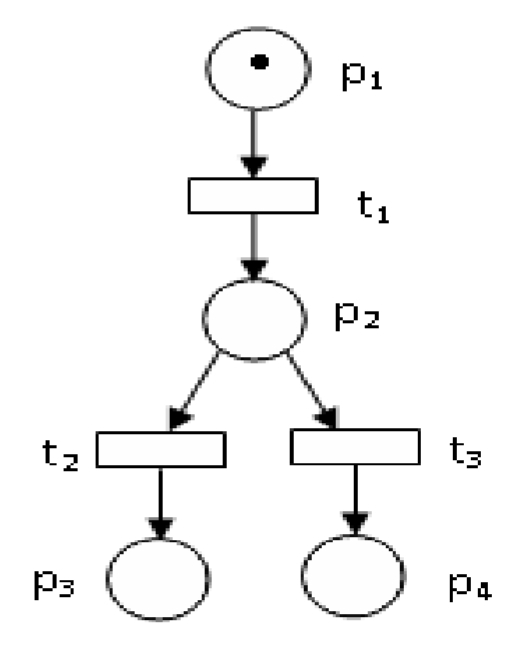
\includegraphics[width=0.4\linewidth]{images/pitref02PNG}
	\caption{ Réseau de Pétri marqué }
	\label{fig:pitref02png}
\end{figure}

Pour le réseau de la (Figure \ref{fig:pitref02png}) .

$ P= \{p1, p2, p3, p4\}$ et $T= \{t1, t2, t3\}  $

 
 \begin{figure}[H]
 	\centering
 	
 	\begin{subfigure}[b]{0.4\textwidth}
 	 \[
 	 pre=
 	 \begin{pmatrix}
 	 1 & 0 & 0 \\
 	 0 & 1 & 1 \\
 	 0 & 0 & 0 \\
 	 0 & 0 & 0
 	 \end{pmatrix}
 	 \]
 	  		\caption{La matrice pré}
 	\end{subfigure}
 	\hfill
 	\begin{subfigure}[b]{0.4\textwidth}
 \[	post=
 	\begin{pmatrix}
 		1 & 0 & 0 \\
 		0 & 1 & 1 \\
 		0 & 1 & 1 \\
 		0 & 0 & 0 
 	\end{pmatrix}
 	\]
 		\caption{La matrice post}
 	\end{subfigure}
 

	
	\begin{subfigure}[b]{0.4\textwidth}
		\[
		C=
		\begin{pmatrix}
		-1 & 0 & 0 \\
		0 & -1 & -1 \\
		0 & 1 & 0 \\
		0 & 0 & 1
		\end{pmatrix}
		\]
			\caption{La matrice d'incidence}
	\end{subfigure}
	\hfill
	\begin{subfigure}[b]{0.4\textwidth}
		\[	M=
		\begin{pmatrix}
		1  \\
		0  \\
		0  \\
		0 
		\end{pmatrix}
		\]
			\caption{Le vecteur de marquage M }
	\end{subfigure}
	
\end{figure}

Le marquage du RdP présenté à la Figure 3 est donné par : 
	\[	M=
\begin{pmatrix}
1  \\
0  \\
0  \\
0 
\end{pmatrix}
\]
On appelle marquage initial, noté M0, le marquage à l’ instant initial (t = 0). 
\end{exmp}
 

\subsection{ L'aspect comportemental }

Le comportement d'un réseau de Pétri est déterminé par sa structure et par son état. Pour exprimer l'état d'un réseau de Pétri, les places peuvent contenir des jetons qui ne sont que de simples marqueurs. .[1] 
\subsubsection{L’état dans un réseau de Pétri  }
Dans la théorie des réseaux de Pétri, l'état d'un réseau est souvent appelé marquage du réseau qui est définit par la distribution des jetons sur les places. Le marquage d'un réseau   de 
Pétri $ R= (P, T, W) $ est défini par la fonction de marquage $  M : P \to N $. 

Un réseau de Pétri marqué est dénoté par $ \sum = (P, T, W, M_{0}) $ où $M_{0}$ est le marquage initial. Le comportement d'un réseau de Pétri marqué est déterminé par ce qu'on appelle règle de franchissement. 

\subsubsection{ Franchissement d’une transition }
Une règle de franchissement est une simple relation de transition qui définit le changement d'état dans un réseau marqué lors de l'exécution d'une action. Afin de définir une règle de franchissement, il est nécessaire de formaliser quand le réseau peut exécuter une action:  on  dit  qu'une  transition $t \in T$ peut  être  franchie  à  partir  d'un  marquage  M  (qui représente l'état du système à un instant donné) si et seulement si chaque place d'entrée $p  \in$$^{*}t$ de la transition t contient au moins un nombre de jetons qui est supérieur ou égal au poids de l'arc reliant cette place d'entrée p avec la transition t  tel que:   $M(p)   \geq W(p, t)  \forall p \in P$. Une règle de franchissement est définie par $M'(p) = M (p) - W(p, t) + W(t, p)$ pour  tout $p \in P$, ce qui veut dire que lorsque la transition t est franchie à partir d'un marquage M, il faut saisir  W(p, t) jetons à partir de chaque place d'entrée à la transition t et déposer W(t, p) jetons dans chaque place de sortie de la transition t ce qui permet de produire un nouveau marquage M'. 

Le franchissement d'une transition t dénoté par $M[t > M' $est dite l'occurrence de t. On  dit que deux transitions t1, t2  (pas nécessairement distinctes) sont franchies en concurrence par un marquage M  si et seulement si $ M (p) \geq W(p, t_{1}) + W(p, t_{2})$ pour toute $p \in P$. .[3] 

Cette vision de l'exécution concurrente de deux transitions dans un RdP est contradictoire avec celle qui impose que deux occurrences de transition sont parallèles si et seulement si : elles sont causalement indépendantes et n'ont pas une relation de conflit entre eux. Deux occurrences sont en conflit si l'un des deux peut avoir lieu mais pas toutes les deux.


\subsubsection{L'exécution d'un réseau de Pétri }

\subsubsection*{Exécution séquentielle }
\begin{enumerate}
\item \textbf{Séquence de franchissement:}
 Une séquence de franchissement « s » est une suite de transitions (t1, t2, …, tn) qui permet, à partir d’un marquage « M », de passer au marquage « M’ » par le franchissement successif des transitions définissant la séquence.
  \item \textbf{Marquage accessible :}Le marquage d’un Réseau de Pétri à un instant donné est une vectrice colonne dont la valeur de la Ième composante est le nombre de marques dans la place $P_{i}$ à cet instant.
  
  
  
  Le franchissement d’une transition conduit à un changement du marquage. Le passage du marquage $M_{k}$ au marquage $M_{l}$ par franchissement de la transition $T_{j}$ est noté :$ M_{k} (T_{j } > M_{l}$. Le nombre de marques dans la place $P_{i}$ pour le marquage Mk est noté $M_{k}(P_{i})$. A partir d’un Même marquage, il peut être possible de franchir plusieurs transitions, menant ainsi à des marquages différents. L’ensemble des marquages accessibles à partir du marquage $M_{0}$ est l’ensemble des marquages obtenus à partir de $ M_{0}$ par franchissements successifs d’une ou plusieurs transition(s). Cet ensemble est noté $ A(R ; M_{0})$. [3]  
  
  \item  \textbf{Graphe de marquage :}
  On peut représenter l’ensemble des marquages accessibles par un graphe si ce dernier et fini. Le graphe de marquage  a comme sommet l’ensemble des marquages accessibles $A(R,M_{0})$. Un arc orienté relie deux sommet $M_{i}$ et $M_{j}$ s’il existe une transition t franchissable permettant de passer d’un marquage à un autre $M_{i} [t>M_{j}$ . Les arcs du graphe sont étiquetés par les transitions correspondantes. [3] 
  
  
  \begin{exmp}
   \end{exmp}
\begin{figure}[H]
	\centering
	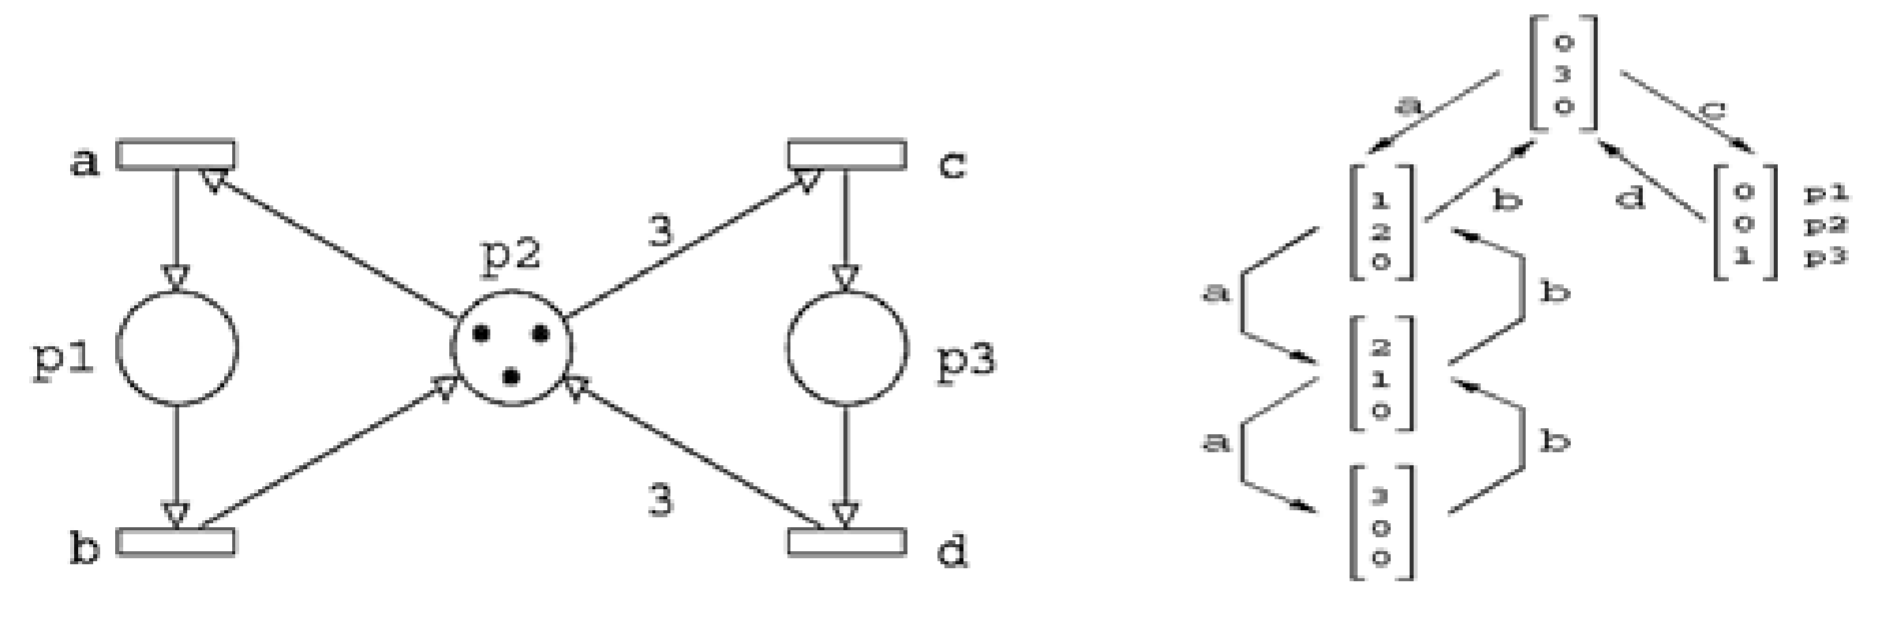
\includegraphics[width=1\linewidth]{images/pitrif03}
	\caption{Graphe de Marquage }
	\label{fig:pitrif03}
\end{figure}

  
  \item \textbf{L'exécution séquentielle d'un réseau de Pétri }
  
  L'exécution séquentielle d'un réseau de Pétri est définie en termes d'un ensemble de séquences d'occurrences. Une séquence d'occurrences est une séquence de transitions franchissables dénotée par $ \sigma =M_{0} t_{1} M_{1} t_{2}…$tel que $M_{i-1}[t_{i} > M_{i}$. Une séquence$ t_{1} t_{2}…$ est une séquence de transitions (commencée par le marquage M) si et seulement si il existe une séquence d'occurrences M0t1M1... avec $M=M_{0}$. Si la séquence finie $t_{1} t_{2}…t_{n}$ conduit à un nouveau marquage M' à partir du marquage M, on écrit $M[t_{1} t_{2}…t_{n} > M’$ ou simplement $M[t_{1} t_{2}…t_{n} >  si $ on ne veut pas spécifier le marquage résultat. [3] 
  
  
  
  
  
\end{enumerate}



\subsubsection*{Exécution concurrente }


Une exécution concurrente d'un réseau de Pétri est une exécution dans laquelle  plusieurs transitions peuvent se franchir en même temps, elle est souvent déterminée par la notion de processus. Ceci permet de donner une interprétation de la concurrence dans un réseau de Petri selon la sémantique basée sur la vraie concurrence (sémantique d'ordre partiel) qui est interprétée dans la théorie des réseaux de Pétri par un type spécial de réseaux appelés réseaux d'occurrences. [3] 



 \section{Réseaux particuliers }



\section{Propriétés des réseaux de Petri}
il existe un certain nombre de propriétés qui ont été définis pour les réseaux de Petri, à savoir, le caractère borné, la réinitilisation la vivacité , la conservation, la terminaison (Diaz, 2001). Certaines de ces propriétés sont dites propriétés dynamiques car elles dépendent du marquage initial et sont liées à l'évolution du réseau,alors que d'autres sont dites propriétés statiques du fait qu'elles soient liées à la typologie du réseau et indépendantes du marquage initial.

\subsection{Réseau K-borné }
\begin{defn}\textbf{\textbf{(Réseau de Petri borné):}}\\
	Une place $ P_{i} $ est bornée pour un marquage initial $ M_{0} $ si pour tout marquage accessible à partir de $ M_{0} $, le nombre de jetons dans $P_{i}$ reste borné. Elle est dite k-bornée si le nombre de jetons dans $ P_{i} $ est toujours inférieur ou égal à k. Un RdP est(k) borné si tout esses places sont(k)bornées.
	
\end{defn}

\begin{exmp}
	Un RdP peut ne pas être borné. Sur l'exemple représenté à la (figure \ref{fig:rdpborn}), la transition $ T_{1} $ admet la place $ P_{1} $ comme unique place d'entrée.La place P1 a un jeton:la transition $ T_{1} $
\end{exmp}

\begin{figure}[h]
	\centering
	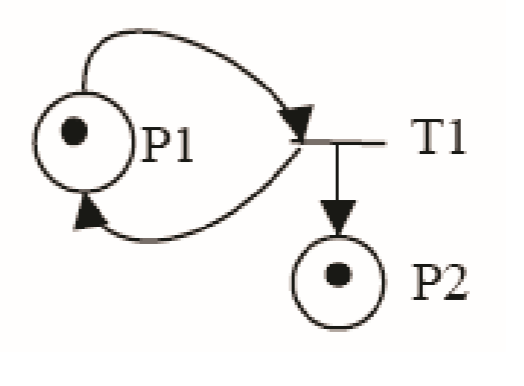
\includegraphics[width=0.5\linewidth]{images/Rdpborn}
	\caption{Réseau de Petri non borné}
	\label{fig:rdpborn}
\end{figure}

est franchissable. Comme $ P_{1} $ est aussi place de sortie de $ T_{1} $,le franchissement de $ T_{1} $ ne change pas le marquage de $ P_{1} $.La transition $ T_{1} $ est donc franchissable en permanence et peut donc être franchie un nombre de fois infini.Chaque franchissement de $ T_{1} $ ajoute un jeton dans $ P_{2} $ dont le marquage va donc tendre vers l'infini.

\begin{defn}\textbf{Réseau de Petri sauf:}\\
	Un RdP est sauf ou binaire pour un marquage initial M0 s'il est un borné.
	
\end{defn}

\subsection{Réseau vivant }
\begin{defn}\textbf{La vivacité:}\\
	Une transition $ T_{j} $ est vivante pour un marquage initial $ M_{0} $ si pour tout marquage accessible $ M_{k} $ , il existe une séquence de franchissement $ S $ à partir de $ M_{k} $ contenant $T_{j}: M_{k} \in^{*} M_{0},   \exists S,M_{k}| S>$ et $S = ... T_{j} ...$
	\\
	
	Si une transition $ T_{j} $ est vivante alors, à tout instant, on sait que $ T_{j} $ peut être franchie dans le futur. Dans le cas d'un réseau de Petri modélisant un système fonctionnant en permanence, si une transition n'est pas vivante et si une fonction du système est associée au franchissement de cette transition,ce la veut dire qu'à partir d’un certain instant ,cette fonction ne sera plus disponible dans le futur, ce qui peut traduire une erreur ou une panne.
	
\end{defn}

\begin{figure}[H]
	\centering
	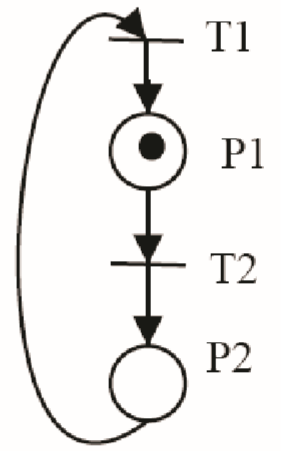
\includegraphics[width=0.2\linewidth]{images/Petrivivant}
	\caption{Réseau de Petri vivant}
	\label{fig:petrivivant}
\end{figure}

\begin{defn}\textbf{Blocage:}\\
	Un blocage (ou état puits)est un marquage pour lequel aucune transition n'est validée.
\end{defn}


Un réseau de Petri est dit sans blocage pour un marquage initial $M_{0}$ si aucun marquage accessible n'est un blocage.

\begin{figure}[H]
	\centering
	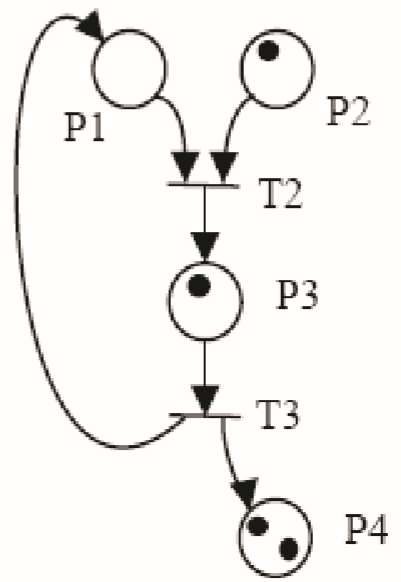
\includegraphics[width=0.25\linewidth]{images/Petribloquant}
	\caption{Exemple de réseau de Petri bloquant}
	\label{fig:petribloquant}
\end{figure}

Le réseau de Petri de la (Figure \ref{fig:petribloquant}), par exemple ,a pour blocage le marquage: 
$M = (1,0,0,1)$.

\subsection{Réseau réinitialisable }
\begin{defn} \textbf{(états d' accueil et Réseau de Petri réinitialisable ) }\\
	Un RdP a un état d’accueil $ M_{a} $ pour un marquage initial $ M_{0} $ si pour tout marquage accessible $ M_{k} $ à partir de $ M_{0} $, il existe une séquence de franchissement permettant d'atteindre le marquage
	$M_{a}: \forall M_{k} \in^{*} M_{0},   \exists S_{j},M_{k}|S_{j}>M_{a}$
\end{defn}
Un RdP est réinitialisable pour un marquage initial $ M_{0} $ si $ M_{0} $ est un\\
état d'accueil.
\\

Si un réseau de Petri présente un état d’accueil, il est facile de vérifier s’il est sans blocage et d'étudier sa vivacité.

\section{ Réseaux de Pétri de haut niveau }
Dans la pratique, on est amené à modéliser toute sorte de système, à savoir les protocoles de communication, les systèmes de production, les systèmes réactifs, les systèmes temps réel, etc. Cette variété de systèmes a poussé les chercheurs à étendre la théorie des RdPs en introduisant beaucoup de concepts relatifs à chaque domaine d’application. Ces efforts ont donné naissance aux RDPs de haut niveau tels que les RDPs colorés, hiérarchiques, temporisés et autres. [6] 
\subsection{Les réseaux de Petri colorés}
Les réseaux colorés(Jensen, 1997)ont été introduits afin de modéliser des systèmes complexes tout en gardant les possibilités de vérification. Lorsque le nombre d'entités du système à modéliser est important,la taille du réseau de Petri devient rapidement énorme,et si les entités présentent des comportements similaires, l'usage des réseaux colorés permet de condenser le modèle. En effet, une couleur est une information attachée à un jeton. Cette information permet de distinguer des jetons entre eux et peut être de type quelconque. Par conséquent, une place peut contenir des jetons de différentes couleurs et une transition peut être franchie de différentes manières, selon la couleur. Ceci est réalisé en attachant un domaine de couleur à chaque place et à chaque transition. Ainsi, les arcs ne sont pas seulement étiquetés par le nombre de jetons mais aussi par leurs couleurs.Le franchissement d'une transition est alors conditionné par la présence dans les places en entrée du nombre de jetons nécessaires, qui en plus satisfont les couleurs qui étiquettent les arcs. Après le franchissement d'une transition,les jetons qui étiquettent les arcs d'entrée sont retirés des places en entrée tandis que ceux qui étiquettent les arcs de sortie sont ajoutés aux places en sortie de cette transition.

Ainsi,pour un même système,le nombre de comportements qui peuvent être exprimés par un réseau coloré est nettement plus élevé qu’avec un réseau simple. Ce sont des réseaux très adaptés aux architectures distribuées.D'autant plus qu`a tout réseau coloré correspond un réseau de Petri simple qui lui est isomorphe.Ce ci permet donc d'exploiter les mêmes techniques d'analyse que celles développées pour les réseaux simples en plus d'autres qui ont été complétées et adaptées aux réseaux colorés telle que le support de la
hiérarchisation.

\begin{defn}\textbf{Réseau de Petri Colorés:}\\
	Un réseau de Petri Coloré (CPN) et un tuple $(\bigtriangleup,P,T,Arc,Noeud,Couleur,Grade,E,M_{0}) $ où :
	
	
\end{defn}


\begin{itemize}
	\item\textbf{ $\bigtriangleup$:}  est un ensemble de domaines de couleurs (chaque domaine est un ensemble fini et non vide ).
	\item \textbf{$ Arc $:} est un ensemble fini d'arcs tel que $P \cap Arc = T \cap Arc = \emptyset $
	\item \textbf{$Nœud$}:  est la fonction $Nœud$ ,$Nœud$ : $Arc \longrightarrow	P \times T \cup T \times P $.
	
	\item   \textbf{$ Couleur $} : $P \longrightarrow PowerSet(\bigtriangleup)$. $Couleur(p)$ est la fonction couleur qui associe à chaque place un domaine de couleur.
	
	\item \textbf{$ Garde $}: est une garde, qui fait correspondre à chaque transition une expression booléenne.Les variables de la garde appartiennent à $\bigtriangleup$.
	\item \textbf{$ E $}: est l'application qui associe à chaque arc, un élément de Couleur(p)MS où p est une place appartenant à l'arc. E indique le nombre de jetons colorés à recevoir de la place qui se trouve en entrée de la transition,et le nombre de ceux à produire dans la place qui se trouve en sortie. 
	
	\item \textbf{$ M_{0} $}: est l'application qui associe à chaque place p,un élément de Couleur(p) $ M_{S} $. $ M_{0}$ (p)indique la distribution initia le des jetons colorés dans la place p.
	
\end{itemize}



De maniéré générale,un marquage M d’un réseau coloré est une application qui associe à chaque place p, un élément de Couleur(p)MS. M(p) est un multi-ensemble sur Couleur(p)qui indique les marques colorées présentes dans la place p au marquage M. L'état du modèle est défini par un marquage coloré.


\subsection{Les réseaux de Pétri à Objet }


Les réseaux de Pétri objet (OPN) étendent le formalisme des réseaux de Pétri colorés avec une intégration complète des propriétés orientées objet y compris l'héritage le polymorphisme et la liaison dynamique, l'orientation objet fournit des primitives de structuration puissant permettant la modélisation des systèmes complexes [6] 

\subsection{Les réseaux de Pétri temporels }

Les réseaux de Pétri temporels sont obtenus depuis des réseaux de Pétri en associant des dates min et max aux transitions.

 Supposons qu’une transition t est devenue sensibilisée pour la dernière fois à l’instant x, alors elle ne peut l’être encore qu’après l’instant x + min(t) et avant l’instant x + max(t), sauf si le tir d’une autre transition a désensibilisé t avant que celle-ci ne soit tirée. Le tir des transitions est de durée nulle. Les réseaux de Pétri temporels expriment nativement des spécifications en «délai». Ils peuvent aussi exprimer des spécifications en «durées». Leur domaine d’application est donc large. [6]


\begin{figure}[H]
	\centering
	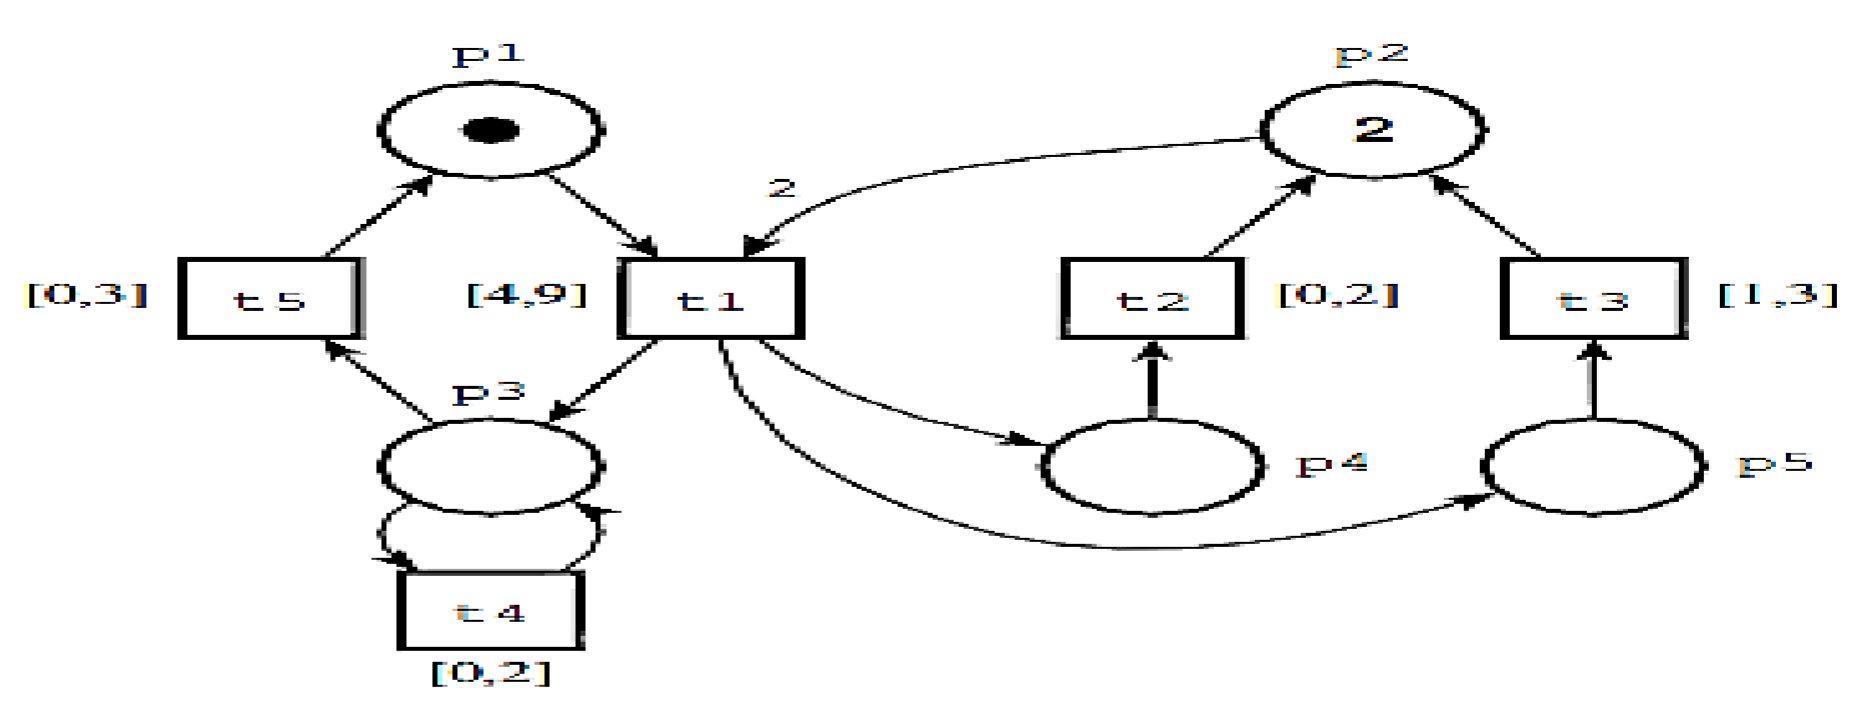
\includegraphics[width=0.7\linewidth]{images/pitrif005}
	\caption{ Exemple de réseau de Pétri temporel }
	\label{fig:pitrif005}
\end{figure}





\section{Réseaux de Petri et workflow
}

Les Réseaux de Petri (RdPs)  constituent un formalisme majeur pour modéliser les processus workflows. Une des forces des RdPs est la base mathématique forte qu'ils offrent avec une représentation graphique. Dans cette section, nous résumons la projection topographique entre concepts de workflow et de RdP  . 

Un processus définit les tâches aussi bien que les conditions pour leur exécution. En utilisant les RdPs, un processus est représenté en conversant sa seule entrée (i.e., un nœud du début) dans une place sans arcs entrants, et sa seule sortie (i.e., nœud de la fin) dans une place sans arcs sortants. Les conditions sont représentées par des places, et les tâches par des transitions. Habituellement, un processus spécifié par RdP devrait accomplir deux exigences : (1) il doit être possible d'accéder à tout moment un état pour lequel il y a un jeton dans la place finale, et (2) quand il y a un jeton dans la place finale, tous les autres jetons auraient dû disparaître.

Dans un processus modélisé par un RdP, une transition active correspond à  un workitem , et le tir d'une transition à une instance de l'activité. Certains work-items peuvent seulement être transformés dans une instance d'activité une fois ils sont déclenchés. Un déclencheur pourrait correspondre à une initiative du participant, à un événement externe ou à un signal du temps initié par l'environnement. A chaque transition correspondante à une tâche qui exige un déclencheur, une autre place d'entrée est ajoutée. Une occurrence du déclencheur apporte un jeton dans cette place supplémentaire. Le jeton est consommé une fois la transition appropriée est franchie. Un échec pendant l'exécution d'une tâche exige un 'rollback' (i.e., revenir à l'état antérieur au début de l'activité). Quand une activité sera complétée avec succès, des changements deviennent définitifs.

\subsection{Modélisation de workflow avec les réseaux de pétri }


Plusieurs recherches ont recommandés l'utilisation des réseaux de pétri pour la modélisation de workflow, et cela à cause de plusieurs facteurs

\subsubsection{Une sémantique formelle } 

Rend la spécification de workflow non ambigüe. L’interprétation de ces spécifications peut être définie mathématiquement.

\subsubsection{Techniques d’analyse} 

Ils existent plusieurs techniques d’analyse de propriétés qualitatives et quantitatives de modèle de workflow à base des réseaux de pétri, une des propriétés qualitatives est de vérifier l’occurrence d’un inter blocage en vérifiant l’accessibilité de toutes les tâches du réseau 

\subsubsection{Expressivité}
Les réseaux de pétri peuvent exprimer la structure des processus ainsi que leurs dynamisme, y compris la concurrence (le parallélisme). Ils servent aussi comme langage pour la définition de la structure d’un processus, simulation de processus et la gestion de workflow


\subsection{Workflow à base de réseaux de pétri (WF-net) }
La modélisation de workflow en terme de réseaux de pétri consiste à modéliser le comportement dynamique du système en représentant les tâches sous forme de transitions, les conditions sous forme de places et les cas sont représentés par les jetons. Les réseaux de pétri qui permettent de modéliser les workflows sont appelés WF-net (réseaux de workflow).

\begin{defn}
\textbf{(Wf-nets):}  Le réseau de pétri qui permet de modéliser le contrôle de flux d’un workflow est appelé un WF-net  (réseaux workflow) Ssi:

\begin{enumerate}
\item Il existe une seule place source $i \in P$ avec $ ^{*}i = \emptyset $ . (i début du processus).

\item  Il existe une seule place puits $o \in P$ avec $ ^{*}o = \emptyset $  (o est la fin du processus).

\item  Chaque nœud $x \in (P \cup T) $est sur un chemin de $i$ à $o$. C’est à dire : Chemin $(i, x)$ $\wedge$ Chemin $(x, o)$.



\end{enumerate} 

\begin{figure}[H]
	\centering
	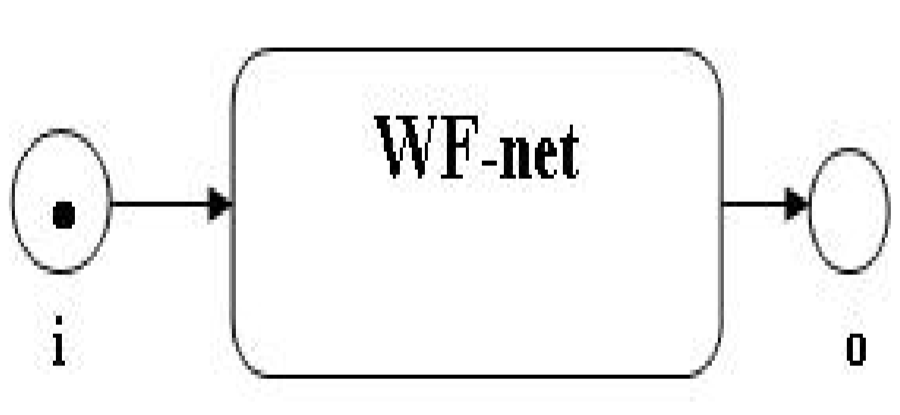
\includegraphics[width=0.5\linewidth]{images/wf-nete006}
	\caption{ Procédure modélisée avec le WF-net }
	\label{fig:wf-nete006}
\end{figure}

\end{defn}
Un réseau de workflow (WF-net) est un réseau de pétri qui possède une seule place d’entrée (i) et une seule place de sortie (o) et puis que n’importe quel cas traité avec la procédure représentée par un WF-net est crée au moment de début de son traitement par le système de gestion de workflow (SGWF) est supprimé une fois que sont traitement est complètement achevé par le SGWF. Cela veut dure que le WFnet spécifie le cycle de vie d’un cas du processus modélisé  .
\begin{rem}
  Un chemin C dans un WF-net d’un nœud $n_{1}$ au nœud $n_{k}$ est une séquence $<n_{1},n_{2},...,n_{k}>$ tel-que $<n_{i},n_{i+1}> \in F $, pour $i=1...k-1$.
  F est la relation de flux. 
\end{rem}

\subsection{Constructions du routage dans un WF-net}
Un réseau de workflow (WF-net) est utilisé pour spécifier le routage de flux dans les cas du workflow, quatre types de routage ont été identifiés :

\subsubsection{Séquentiel :}

Utilisé pour traiter la relation de causalité entre les tâches. Soit deux tâches A et B, si la tâche B et exécutée après l’accomplissement de A, ce comportement peut être modélisé avec un RDP en ajoutant les places pour capter les relations de causalité entre les tâches A et B. La figure \ref{fig:wf003} illustre ce comportement.


\begin{figure}[H]
	\centering
	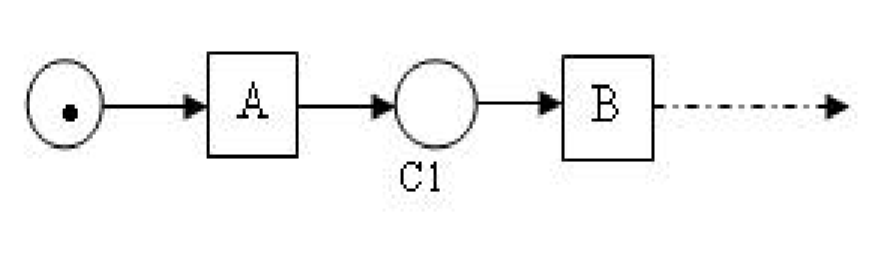
\includegraphics[width=0.7\linewidth]{images/wf003}
	\caption{Routage séquentiel.}
	\label{fig:wf003}
\end{figure}

\subsubsection{Parallèle : }
Utiliser dans le cas où l’ordre d’exécution est moins strict. Par exemple si on a deux tâches B et C qui doivent être exécutées mais dans un ordre arbitraire, la modélisation de ce comportement de routage parallèle comporte deux constructions le AND-split et AND-join.


\begin{figure}[H]
	\centering
	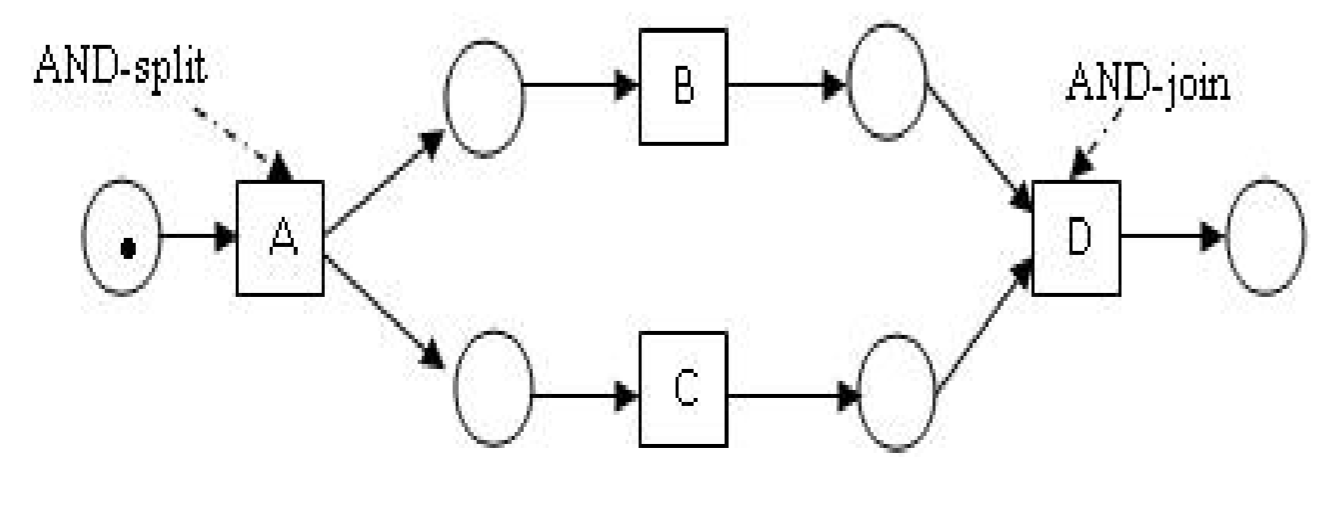
\includegraphics[width=0.7\linewidth]{images/Capture}
	\caption{Routage parallèle.}
	\label{fig:capture}
\end{figure}

\subsubsection{Conditionnel :}

Utilisé pour traiter les cas où le routage de flux peut dépendre des données d’un cas. Il existe deux types de routage conditionnel : \textit{\textbf{le choix non-déterministe}} et \textit{\textbf{le choix déterministe}}. 


\begin{enumerate}

\item \textbf{Choix non-déterministe :} Pour modéliser ce comportement deux constructions sont utilisées OR-Split et OR-join. La figure \ref{fig:wf005} représente un choix entre l’exécution des deux tâches B ou C grâce à un jeton dans la place c2, mais cela permet un choix non-déterministe (l’exécution de B ou de C car les deux tâches sont permises).



\begin{figure}[H]
	\centering
	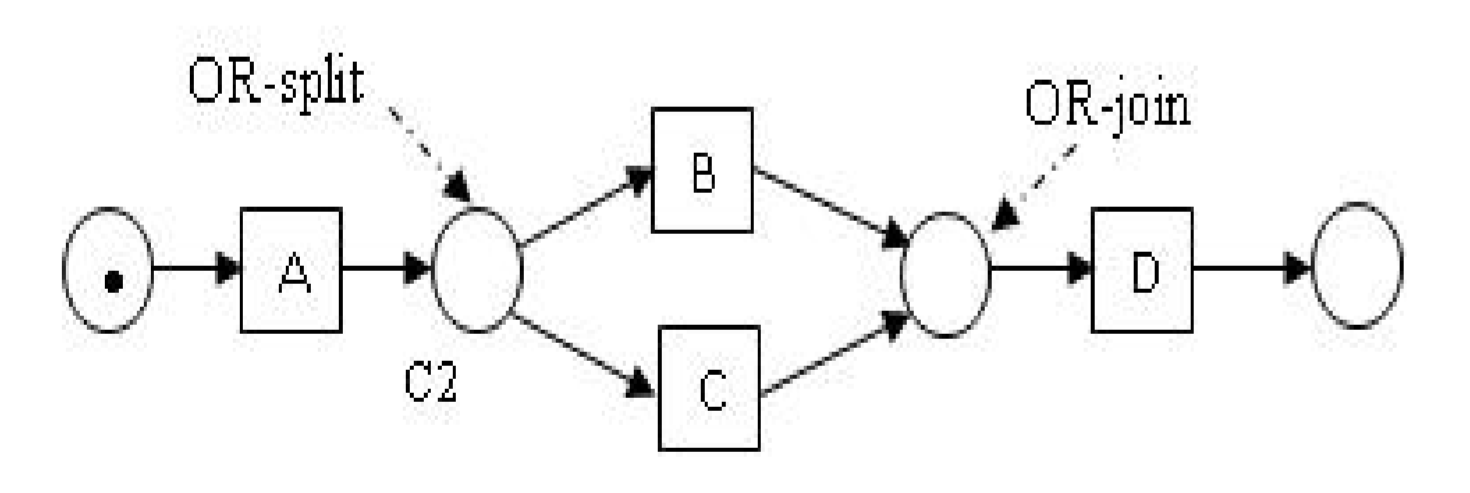
\includegraphics[width=0.7\linewidth]{images/wf005}
	\caption{Routage conditionnel non-déterministe}
	\label{fig:wf005}
\end{figure}



\item \textbf{Choix déterministe : } Le choix entre plusieurs alternatives peut être guidé par les données (ou les attributs) du workflow, dans ce cas c’est un choix déterministe.

Nous pouvons prendre le schéma de la figure précédente et ajouter une pré-condition pour chacune des tâches B et C (en se basant sur un ou plusieurs attributs du workflow).

Il y a une autre façon de modéliser le choix déterministe comme dans la figure suivante. La transition A comporte deux places de sortie c2 et c3 et produit un seul jeton (soit dans c2 ou dans c3). Le choix entre les deux places est basé sur la valeur de l’attribut x.Un symbole spécial est utilisé pour représenté que la tâche A est un OR-split (exclusive OR).


\begin{figure}[H]
	\centering
	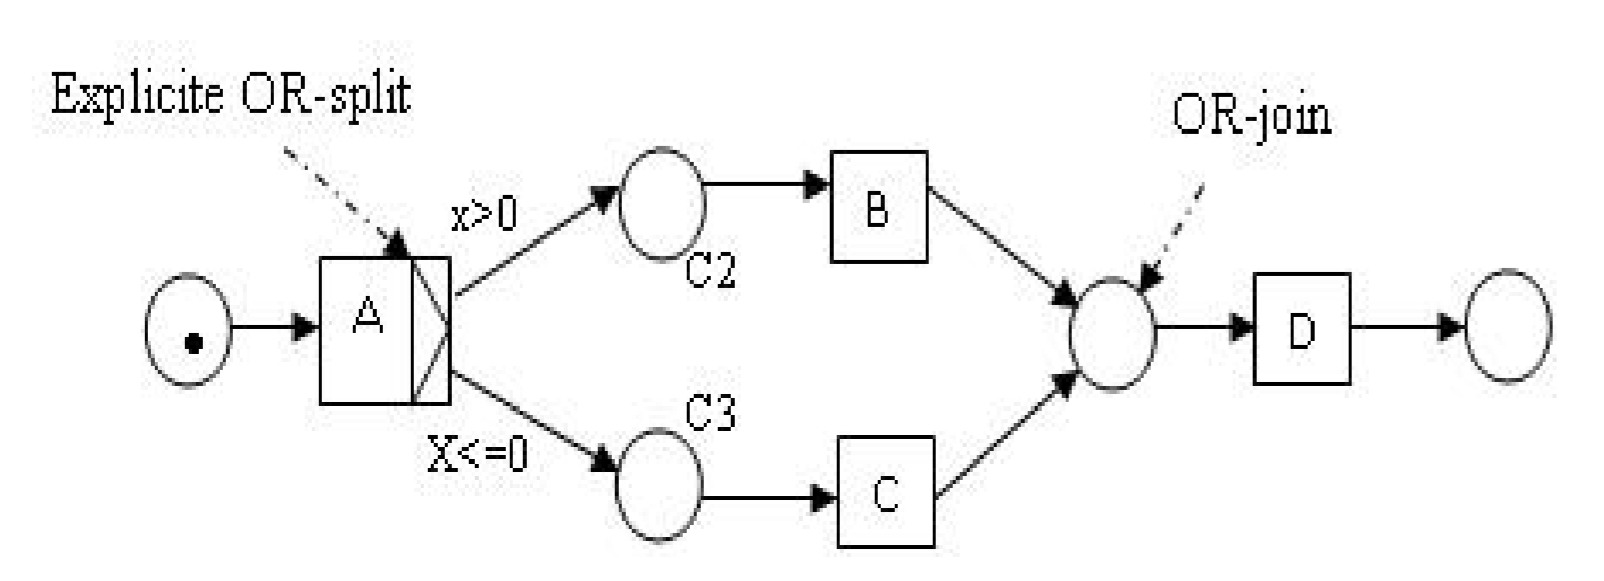
\includegraphics[width=0.7\linewidth]{images/wf006}
	\caption{Choix explicite entre B et C à base de l’attribut x .
	}
	\label{fig:wf006}
\end{figure}

\item \textbf{Itération : } L’itération peut être modélisée en utilisant l’implicite (OR-split, OR-join), l’explicite (OR-split, OR-join). Il est utilisé dans le cas où une ou plusieurs tâches peuvent être exécutées plusieurs fois. La figure suivante montre un exemple d’un modèle de workflow en utilisant un routage itératif.


\begin{figure}[H]
	\centering
	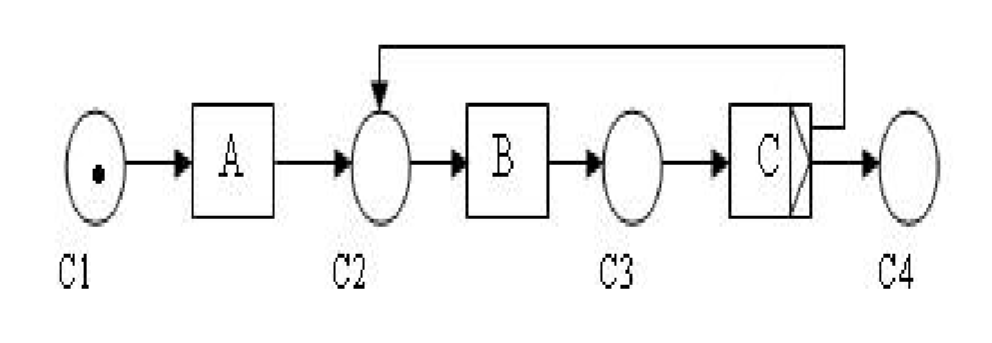
\includegraphics[width=0.7\linewidth]{images/wf008}
	\caption{Itération : B peut être exécutée plusieurs fois}
	\label{fig:wf008}
\end{figure}
\end{enumerate}

\section{Conclusion }





















%\chapter{Implémentation}
%

\section*{Introduction}

\comment{
	Après avoir achevé notre étude de l’existant et étudié de près le système actuel, nous abordons l’étape suivante qui consiste à concevoir le nouveau système en utilisant la modélisation UML. L’objectif de cette étape est de déterminer de façon détaillée et précise ce que le nouveau système devrait faire, afin de répondre aux objectifs attendus. Dans ce chapitre nous allons détailler les objectifs fixés du système,en suite nous détaillons ses fonctionnalités et sa logique de fonctionnement. 
	%Nous présentons aussi 
}




Dans cette parti de pratique et dans ce chapitre  nous parlons sur l'analyse à la conception de travail d'abord on va parler sur   UML  (sa définition,  contente...  ex ). puis identifier les objectifs de projet  spécifications des besoins fonctionnaire et les besoins technique, ensuite la description	 du  diagramme de cas d'utilisation  et pour la conception :une représentation des informations par le diagramme de classe et  le diagramme d'activité  



 \section{Unified Modeling Language (UML):}
 Dans ce qui suit, nous allons donner une brève description d’UML.
 \subsection{ Définition UML }
 L’OMG définit l’UML comme un langage visuel dédié à la spécification,la construction et la documentation des artéfacts d’un système logiciel. Aussi la façon dont tout le monde modélise non seulement la structure de l’application, le comportement et l’architecture, mais aussi des processus d’affaires et la structure des données. Ce langage est conçu pour modéliser divers types de systèmes et de taille quelconque. Il possède une approche entièrement objet couvrant tout le cycle de développement. Le système est décomposé en un ensemble d’objets collaborant [GUIBERT, 2010].
 
 \subsection{Contenu UML}
 
 L’UML comporte 13 diagrammes qui se répartissent en deux catégories [GUIBERT, 2010]. Nous ne mentionnons que les diagrammes que nous utilisons, les autres sont en annexe G. 
 
 \subsubsection{Diagramme structurel : }
 \begin{itemize}
 \item \textbf{Diagramme de classes (Class Diagram) : }ce diagramme décrit la structure statique du système, il définit les classes, leurs attributs et leurs relations. Il est considéré comme le diagramme le plus important.
  \item  \textbf{Diagramme de paquetages (Package Diagram) : }définit les dépendances entres les paquets (groupement d’éléments UML) constituant un modèle. 
 \end{itemize}
 
 
  \subsubsection{Diagramme comportemental  : }
 
  \begin{itemize}
 	\item \textbf{Diagramme de cas d’utilisation (Use Case Diagram) : } pour décrire les besoins des utilisateurs. 
 	\item  \textbf{Diagramme de séquence(Sequence Diagram):}  décrit comment chaque objet interagit avec l’autre et dans quel ordre, sur un axe temporel donné. Ce diagramme sont associés aux diagrammes de cas d’utilisation.
 	. 
 \end{itemize}



\section{Identification des objectifs}
\comment{
Au début du projet, nous nous sommes concentrés sur les besoins qui pourraient normalement être considérés comme un système général et nous avons interrogé les ingénieurs de la société nationaux de retraités    "CNR", qui ont exprimé des besoins importants. 
 
 
 Nos entretiens ont été complétés en suivant les étapes ci-dessous
 
\textbf{ Étape 1:} Choisir les entretiens Afin d'identifier les besoins, nous avons contacté des personnes pouvant fournir des informations utiles et fournir des explications. Les personnes responsables de la production des différentes unités ou entreprises sont les plus appropriées pour répondre à nos questions.
 
\textbf{Étape 2:}
Planification du développement du programme À ce stade de la planification des entretiens, nous avons étudié deux points essentiels:

- Déterminer le contexte général de l'entretien : "CNR",

- Réglage de la date et de l'heure de l'entretien (date). 

\textbf{ Étape 3:} Préparez-vous pour l’entrevue Préparez les questions de développement et les supports pour un processus sans faille (stylos, cartons de réponses, papiers blancs supplémentaires, clé USB).


\textbf{ Étape 4:} Conduisez l’entretien: Commencez le processus d’entretien en vous présentant d’abord, puis en présentant brièvement notre projet, puis en passant l’entretien en interrogeant la personne concernée et en enrichissant sa conversation d’observations et de questions. Intermédiaire.
 
\textbf{ Étape 5:} Après l'entretien Après avoir pris les informations collectées et conclu l'entretien, nous avons décidé de procéder à d'autres entretiens en développant et en nous réunissant à chaque fois.
 
 
 Sur la base de ces entretiens et de l'entretien avec l'enseignant, nous avons pu identifier les spécifications suivantes:
}
 \subsection{Spécifications fonctionnelles }
  Le système doit permettre à l’administrateur  de:
 \begin{enumerate}
\item  	    Générer le modèle. 
\item  	    Gérer Sous-direction. 
\item  	    Gérer les service.
\item  	    Gérer workflow pour les dossier.  
\item  	    Gérer les tâches des service.  
\item  	    Gérer les utilisateur. 
\item  	    Consulte les historique  et la recherche par tâche. 
\item  	    Consulte les historique  et la recherche par dossier et les jours pour chaque tâche. 
\item  	    Consulte bordereau. 
 \end{enumerate}
 Le système doit permettre à l’utilisateur   de :
 \begin{enumerate}
\item  	    Gérer les dossier. 
\item  	    Activé le dossier.    
\item  	    Finir le traitement des dossiers par tâche.    
\item  	    Gérer les  bordereaux.  
\item  	    Accepte le  bordereau.  
\item  	    Refuse  le  bordereau.  
\item  	    Imprimer le  bordereau.  

 \end{enumerate}
 
 
 
 
  \subsection{Spécifications techniques }
 
 
 
  \begin{enumerate}
 	\item  	   Le système doit être déployé sur le cloud.  
 	\item  	   La configuration et la germanisation de code dynamique.  
 	\item  	   Modélisation d'un Workflow Administratif via un interface graphique simple et utile.  
 	
 
 	
 \end{enumerate}
 
 
 
 
 
 
 
 
 
 
 
\subsection{ Diagramme de cas d’utilisation }
 
  \subsubsection{ les acteurs de système  }
 
 Un acteur représente l'abstraction d'un rôle joué par des entités externes (utilisateur, dispositif matériel ou autre système) qui interagissent directement avec le système (réception d’information, etc.). Pour notre application,on a trois acteurs : le premier acteur c'est l'administrateur et le deuxième  c'est utilisateur simple  et le troisième c'est l'utilisateur simple. 
 
\begin{table}[H]
	\begin{tabular}{|l|l|l|}
		\hline
		\multicolumn{1}{|l|}{Acteur} & Type Acteur & Descriptions \\ \hline
	Administrateur	 &  & S’authentifier \\ \cline{3-3} 
		&  & Gérer le Modèle \\ \cline{3-3} 
		&  & Gérer Sous Direction \\ \cline{3-3} 
	 	&  & Gérer les Services \\ \cline{3-3} 	
	 	&  & Gérer les Tâches \\ \cline{3-3} 
		&  & Gérer les Utilisateurs \\ \cline{3-3} 
		& Acteur Principale & Gérer Workflow par BPMN  \\ \cline{3-3} 
				&  & Consulter les Bordereaux  \\ \cline{3-3} 
						&  &Consulter les historique des dossiers\\ \cline{3-3} 
								&  & Gérer les Utilisateurs \\ \hline 
		
  
			Utilisateur réception	 	&Acteur Principal & Créer et Gérer les dossiers  \\ \cline{3-3}  
		&  & Activé les dossiers et ajoute sur wf \\ \hline
 
		Utilisateur Simple	&  & finir le traitement de dossier  \\ \cline{3-3} 
		&  Acteur Principal& Gérer les Bordereaux  \\ \cline{3-3} 
		&  &Gérer les historique des dossiers\\ \hline 
	\end{tabular}
\end{table}
 
 \subsubsection{ Cas d’utilisation }
 Le diagramme des cas d’utilisation suivant illustre les fonctionnalités qu’un simple utilisateur du système, également l’administrateur, peut faire. Ce diagramme a été inspiré des spécifications citées ci-dessus :
 
 \begin{figure}[H]
 	\centering
 	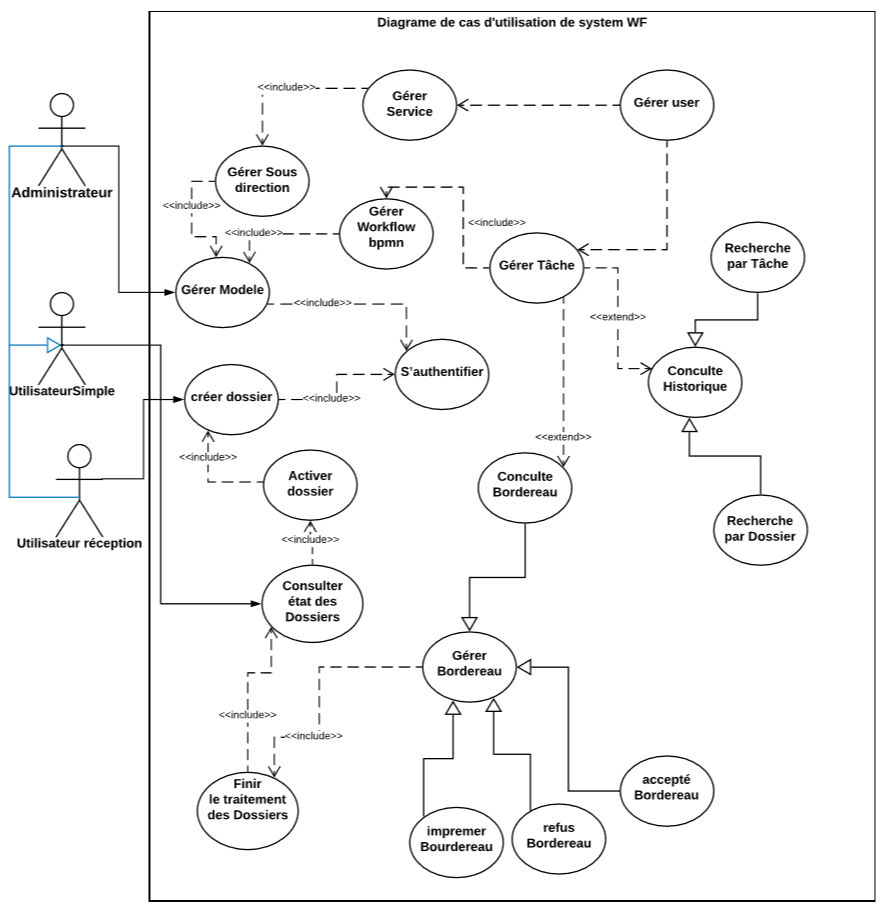
\includegraphics[width=1\linewidth,height=0.8\paperheight]{usercase2}
 	\caption{Diagramme de Cas d’utilisation}
 	\label{fig:usercase2}
 \end{figure}
 
 \subsection{ Documentation des cas d’utilisation fonctionnels }
Nous détaillerons chaque cas d'utilisation avec une description  brève et spécifie  les acteurs principal et les acteurs secondaires, ainsi que les Post-conditions  et les pré-conditions  pour le faire sont la séquence principal et la séquence alternative. 

 \subsubsection{ S’authentifier }
 \begin{table}[H]
 	\centering
 	\begin{tabular}{|l|} 
 		\hline
 	\textbf{	CU :} S’authentifier     \\  	\hline
 		\textbf{ID:}1         \\  		\hline
 		\begin{tabular}[c]{@{}l@{}}\textbf{Description brève :} chaque utilisateur doit s’authentifier\\ auprès de l’application afin de pouvoir \\ utiliser les fonctionnalités du système, tel que la consultation du\\ tableau de bord, la manipulation les rapports... etc. \end{tabular}          \\ 
 		\hline
 		\textbf{Acteurs primaires : }utilisateur, administrateur   \\ 
 		\hline
 		Acteurs secondaires :                                                                                                                                                                                                                                                                                                                                                                                                                                                                                                                                                                                                                                                                                                                                                                             \\ 
 		\hline
 		\begin{tabular}[c]{@{}l@{}}\textbf{Pré-conditions :} – La connexion auprès du serveur d’application doit\\ être réussite. – L’utilisateur \\ doit être enregistré dans le système. \end{tabular}                                                                                                                                                                                                                                                                                                                                                                                                                                                                                                                                                                                                           \\ 
 		\hline
 		\begin{tabular}[c]{@{}l@{}}\textbf{Enchainement principal : }Ce cas d’utilisation commence lorsqu’un\\ utilisateur souhaite accéder à \\ l’application. \\ 1. L’utilisateur saisit le lien de l’application dans barre\\ d’adresse du navigateur. \\ 2. Le serveur répond à l’utilisateur en renvoyant une page\\ d’authentification.\\ 3. L’utilisateur saisit\\ son nom d’utilisateur et son mot de passe et les valide en appuyant sur \\ 4. “Log in”. \\ 5. Le serveur vérifie la validité du nom d’utilisateur et du mot\\ de passe. \\ 6. Le serveur envoie une page d’accueil de l’application à\\ l’utilisateur concerné. \end{tabular}     \\ 
 		\hline
 		Post-conditions : L’utilisateur est connecté.                                                                                     \\ 
 		\hline
 		\begin{tabular}[c]{@{}l@{}}Enchainement alternatif :  \\\begin{tabular}{@{\labelitemi\hspace{\dimexpr\labelsep+0.5\tabcolsep}}l} E1 : La page d’authentification n’apparait pas à l’utilisateur.\end{tabular}\\ * L’enchainement démarre   après le premier point de l’enchainement principal. \\ * Le serveur envoie un message d’erreur à  l’utilisateur. \\\begin{tabular}{@{\labelitemi\hspace{\dimexpr\labelsep+0.5\tabcolsep}}l} E2 : Le nom d’utilisateur ou/et le mot de passe ne sont pas valides.\end{tabular}\\ L’enchainement démarre après le quatrième point de l’enchainement principal. 
 			\\
 			* Le serveur envoie un message d’erreur à l’utilisateur.
 			
 			\\ * Le serveur demande à l’utilisateur de ressaisit le nom d’utilisateur et le mot de passe. \end{tabular}  \\
 		\hline
 	\end{tabular}
 \end{table}







\subsubsection{Créer circuit Workflow}
\begin{table}[H]
	\begin{tabular}{|l|}
		\hline
		\textbf{	CU : }Créer circuit Workflow\\ \hline
		\textbf{	ID }: 12 \\ \hline
		\textbf{	Description brève :}L'administrateur Créer circuit Workflow pour les dossiers \\ \hline
		\textbf{	Acteurs primaires :} L'administrateur  \\ \hline
		\textbf{Acteurs secondaires :}\\ \hline
		\textbf{	Pré-conditions :} L'administrateur est connecté ! \\ \hline
		\begin{tabular}[c]{@{}l@{}}\textbf{Enchainement principal :} Créer circuit Workflow pour les dossiers et \\la création des tâches sur la base de données Normal \end{tabular} \\ \hline
		\textbf{Post-conditions : }Workflow est défier et les tâche a remplier      \\ \hline
		\begin{tabular}[c]{@{}l@{}}\textbf{Enchainement alternatif : }   \\ \end{tabular} \\ \hline
	\end{tabular}
\end{table}







\subsubsection{Gérer les Services}
\begin{table}[H]
	\begin{tabular}{|l|}
		\hline
		\textbf{	CU : }Gérer les Services \\ \hline
		\textbf{	ID }: 22 \\ \hline
		\textbf{	Description brève :}L'administrateur peut Gérer les Services par création, \\ modification et la suppression  \\ \hline
		\textbf{	Acteurs primaires :} L'administrateur  \\ \hline
		\textbf{Acteurs secondaires :}  \\ \hline
		\textbf{	Pré-conditions :} L'administrateur est connecté ! \\ \hline
		\begin{tabular}[c]{@{}l@{}}\textbf{Enchainement principal :}L'administrateur   crée un mouve service au\\ système et peut la   modifier.   \end{tabular} \\ \hline
		\textbf{Post-conditions : } le service ajouté à la BDD  \\ \hline
		\begin{tabular}[c]{@{}l@{}}\textbf{Enchainement alternatif : }    \\\end{tabular} \\ \hline
	\end{tabular}
\end{table}

\subsubsection{Gérer utilisateur  }
\begin{table}[H]
	\begin{tabular}{|l|}
		\hline
		\textbf{	CU : }Gérer utilisateur \\ \hline
		\textbf{	ID }: 12 \\ \hline
		\textbf{	Description brève :}L'administrateur Gérer les comptes des utilisateurs \\ \hline
		\textbf{	Acteurs primaires :} L'administrateur  \\ \hline
		\textbf{Acteurs secondaires :}   \\ \hline
		\textbf{	Pré-conditions :} L'administrateur est connecté !  \\ \hline
		\begin{tabular}[c]{@{}l@{}}\textbf{Enchainement principal :} L'administrateur fit la création des comptes pour les \\utilisateurs. \end{tabular} \\ \hline
		\textbf{Post-conditions : }des comptes utilisateur à crée \\ \hline
		\begin{tabular}[c]{@{}l@{}}\textbf{Enchainement alternatif : } \\ \end{tabular} \\ \hline
	\end{tabular}
\end{table}




\subsubsection{Consulte  Historique   }
\begin{table}[H]
	\begin{tabular}{|l|}
		\hline
		\textbf{	CU : }Consulte  Historique \\ \hline
		\textbf{	ID }: 32 \\ \hline
		\textbf{	Description brève :}L'administrateur peut Consulte  Historique des\\ dossiers leurs état, la recherche \\par dossier ou la recherche par tâche   \\ \hline
		\textbf{	Acteurs primaires :} L'administrateur  \\ \hline
		\textbf{Acteurs secondaires :}   \\ \hline
		\textbf{	Pré-conditions :} L'administrateur est connecté !  \\ \hline
		\begin{tabular}[c]{@{}l@{}}\textbf{Enchainement principal :} -L'administrateur sélectionner le dossier ou la \\ tâche pour la recherche 
		\\ -Résulta afficher l'état des dossiers   \end{tabular} \\ \hline
		\textbf{Post-conditions : }afficher le résulta de la recherche  \\ \hline
		\begin{tabular}[c]{@{}l@{}}\textbf{Enchainement alternatif : } \\ \end{tabular} \\ \hline
	\end{tabular}
\end{table}











 \subsubsection{cas d'utilisation par l'utilisateur réception ou initial   }
l'utilisateur de réception il fait de rôle principal le premier c'est gérer les dossiers le deuxième c'est activer le dossier.
  \subsubsection{Créer Dossiers}
 \begin{table}[H]
 	\begin{tabular}{|l|}
 		\hline
 	\textbf{	CU : }Créer   Dossiers \\ \hline
 	\textbf{	ID }: 2 \\ \hline
 	\textbf{	Description brève :} chaque utilisateur pus Créer  et enregistre les noves   Dossiers \\ \hline
 	\textbf{	Acteurs primaires :} utilisateur réception ou initiale, \\ \hline
 		\textbf{Acteurs secondaires :} simple utilisateur \\ \hline
 	\textbf{	Pré-conditions :} L’utilisateur doit être  connecte ou  le système. \\ \hline
 		\begin{tabular}[c]{@{}l@{}}\textbf{Enchainement principal :} Ce cas d’utilisation commence   lorsqu’un utilisateur\\  souhaite accéder à  l’application. \\   1.      L’utilisateur sélectionner de ajouté Nouvo dossier. \\   2.      system répond à l’utilisateur en afficher un formuler de enregistrement.\\   3.       L’utilisateur saisit le   code  et le nom prénom et numéro de typhon\\   de personne de dossier    \\   4.      L’utilisateur vérifier le dossier  et  sélectionner   les chants  présent.\\  en appuyant sur « enregistrer ».\\   5.      Le system envoie une page des dossiers.\end{tabular} \\ \hline
 		\textbf{Post-conditions : }le dossier   est enregistré et ajouté dans le system. \\ \hline
 		\begin{tabular}[c]{@{}l@{}}\textbf{Enchainement alternatif : }    \\  \textbf{ E1:} Le code  de Dossier n’est pas valides ou/et déjà existe.\\   o    L’enchainement démarre après le quatrième point de l’enchainement principal. \\   o     Le serveur envoie un message d’erreur à  l’utilisateur. \\   o   Le serveur demande à l’utilisateur de ressaisit le code de Dossier.\end{tabular} \\ \hline
 	\end{tabular}
 \end{table}
 
 




\subsubsection{Activer Dossiers}
\begin{table}[H]
	\begin{tabular}{|l|}
		\hline
		\textbf{	CU : }Activer Dossiers \\ \hline
		\textbf{	ID }: 3 \\ \hline
		\textbf{	Description brève :}L'utilisateur peut activer le statut du dossier et commencer \\au  début de la tâche "Ajouter au flux de travail", \\ après avoir rempli tous les documents.    \\ \hline
		\textbf{	Acteurs primaires :} utilisateur réception ou initiale, \\ \hline
		\textbf{Acteurs secondaires :} simple utilisateur \\ \hline
		\textbf{	Pré-conditions :} Le Dossier  doit être enregistré dans le système.\\ \hline
		\begin{tabular}[c]{@{}l@{}}\textbf{Enchainement principal :} \\ 1.      L’utilisateur sélectionner de ajouté la liste des dossier.  \\ 
			2.      system répond à l’utilisateur en afficher  les liste des dossier \\ \{"tous la liste","liste activer ","liste non activer" \}. \\  
			3.       L’utilisateur sélectionner  dossier    \\ 
			4. le system  répond à l’utilisateur en afficher le détaille, est aprés\\  en appuyant sur "Activer". \\  
			5. le system vérifie id "code" de dossier et activer leur état \end{tabular} \\ \hline
		\textbf{Post-conditions : }le dossier  est activé dont la premier tache.  \\ \hline
		\begin{tabular}[c]{@{}l@{}}\textbf{Enchainement alternatif : } \end{tabular} \\ \hline
	\end{tabular}
\end{table}



\subsubsection{cas d'utilisation par l'utilisateur simple  }
l'utilisateur il fait de rôle principal  : consulter l'état du dossier pour finir le traitement créer des bordereaux    pur transfert les dossier (imprimer   et refus ou accepté  les bordereaux).

 
 
\subsubsection{Consulter état des Dossiers}
\begin{table}[H]
	\begin{tabular}{|l|}
		\hline
		\textbf{	CU : }Consulter état des Dossiers \\ \hline
		\textbf{	ID }: 4 \\ \hline
		\textbf{	Description brève :}L'utilisateur peut visualiser le statut des dossiers en cours \\ de traitement  en fonction de sa tâche et voir tous les dossiers envoyés par une \\autre tache.     \\ \hline
		\textbf{	Acteurs primaires :} utilisateur  \\ \hline
		\textbf{Acteurs secondaires :}  \\ \hline
		\textbf{	Pré-conditions :} 
		\\ - Le Dossier  doit être Activé dans le système.
		\\ -  L’utilisateur doit être  connecte ou  le système.
		\\ \hline
		\begin{tabular}[c]{@{}l@{}}\textbf{Enchainement principal :} \\ 1.      L’utilisateur sélectionner  le statut des dossiers.  \\ 
			2.      system répond à l’utilisateur en afficher  les liste des dossier encore de traitement\\ ou les noves  dossiers envoyés    \end{tabular} \\ \hline
		\textbf{Post-conditions : }L'utilisateur   visualiser le statut  des dossiers par sa tâche. \\ \hline
		\begin{tabular}[c]{@{}l@{}}\textbf{Enchainement alternatif : } \end{tabular} \\ \hline
	\end{tabular}
\end{table}



\subsubsection{Finir le traitement  des Dossiers}
\begin{table}[H]
	\begin{tabular}{|l|}
		\hline
		\textbf{	CU : }Finir le traitement  des Dossier \\ \hline
		\textbf{	ID }: 5 \\ \hline
		\textbf{	Description brève :}L'utilisateur peut sélectionner liste des dossier et finir\\ leur traitement   \\ \hline
		\textbf{ Acteurs primaires :} utilisateur  \\ \hline
		\textbf{Acteurs secondaires :}  \\ \hline
		\textbf{	Pré-conditions :} 
		\\ - Le Dossier  doit être Activé dans    la tâche de l'utilisateur. 
		\\ -  L’utilisateur doit être  connecte ou  le système.   
		\\ \hline
		\begin{tabular}[c]{@{}l@{}}\textbf{Enchainement principal :} \\ 1.      L’utilisateur sélectionner la liste  des dossiers pour finir le traitement en payent \\sur "terminer",   \\ 
			2.      system répond à l’utilisateur et terminer le traitement des dossier par \\ changer état et la date fin de traitement.   \end{tabular} \\ \hline
		\textbf{Post-conditions : }L'utilisateur   finir le traitement   des dossiers par sa tâche. \\ \hline
		\begin{tabular}[c]{@{}l@{}}\textbf{Enchainement alternatif : } \end{tabular} \\ \hline
	\end{tabular}
\end{table}






\subsubsection{Gérer Bordereau}
\begin{table}[H]
	\begin{tabular}{|l|}
		\hline
		\textbf{	CU : }Gérer Bordereau   \\ \hline
		\textbf{	ID }: 6 \\ \hline
		\textbf{	Description brève :}L'utilisateur peut sélectionner liste des dossier et \\Gérer un  Bordereau  \\   \hline
		\textbf{ Acteurs primaires :} utilisateur  \\ \hline
		\textbf{Acteurs secondaires :}  \\ \hline
		\textbf{	Pré-conditions :} 
		\\ - Le Dossier  doit être terminer le traitement  dans    la tâche de l'utilisateur.  
		\\ -  L’utilisateur doit être  connecte ou  le système.   
		\\ \hline
		\begin{tabular}[c]{@{}l@{}}\textbf{Enchainement principal :} \\ 1.      L’utilisateur sélectionner la liste  des dossiers et sélectionner \\le suivant tache  pour transfert    \\ 
			2.  system répond à l’utilisateur et créer  nounous bordereau et afficher la liste\\ de bordereau correspondre a leur tache. 
		  \\ 
		3.  L’utilisateur put imprimer et accepte ou refuse le bordereau.     \end{tabular} \\ \hline
		\textbf{Post-conditions : } L'utilisateur  créer bordereau et transfert les dossier \\si le bordereau accepte par validation d'un utilisateur de la tâche reçu.  \\ \hline
		\begin{tabular}[c]{@{}l@{}}\textbf{Enchainement alternatif : }  
	\textbf{	E1:bordereau refuse. }
	\\ * renvoyer a la tâche président tous les dossier   
	
 \end{tabular} \\ \hline
	\end{tabular}
\end{table}
 
 \section{ Représentation des informations }
 \subsection{Diagramme de Classe}
\begin{figure}[H]
	\centering
	\includegraphics[width=1\linewidth,height=0.6\paperheight]{images/class01}
	\caption{Diagramme de Classe}
	\label{fig:class01}
\end{figure}

  \subsubsection{Conception détaillée} 
Nous allons définir pour chaque classe ses attributs et leur types,  ainsi que les méthodes qu’elle offre. Dans le but d’alléger le rapport, nous avons jugé essentiel de ne citer  les classes que nous avons conçu.  
 
 

\subsubsection*{La classe  Sous-Direction}
\begin{table}[H]
  \centering\setlength\tabcolsep{0.8cm}
	\begin{tabular}{|l|l|l|}
		\hline
		\textbf{Attribut}  & \textbf{Type} & \multicolumn{1}{l|}{\textbf{Méthodes}} \\ \hline
	
		id & long & getId() et setId()\\ \cline{1-2}
		nom & String  & getNom() et setNom() \\ \cline{1-2}
	services	& $ List<Service> $ & getServices() et setServices()   \\ \hline
	\end{tabular}
\end{table}
\subsubsection*{La classe Service}
\begin{table}[H]
	\centering
	\begin{tabular}{|l|l|l|}
		\hline
		\textbf{Attribut}  & \textbf{Type} & \multicolumn{1}{l|}{\textbf{Méthodes}} \\ \hline
		
		id & long & getId() et setId()\\ \cline{1-2}
		nom & String  & getNom() et setNom() \\ \cline{1-2}
				sous-Direction & Sous-Direction  & getSous-Direction() et setSous-Direction() \\ \cline{1-2}
		myTasks	& $ List<MyTask> $ & getMyTasks() et setMyTasks()   \\ \hline
	\end{tabular}
\end{table}


\subsubsection*{La classe MyTask}
\begin{table}[H]
	\centering
	\begin{tabular}{|l|l|l|}
		\hline
		\textbf{Attribut}  & \textbf{Type} & \multicolumn{1}{l|}{\textbf{Méthodes}} \\ \hline
		
		id & long & getId() et setId()\\ \cline{1-2}
		nom & String  & getNom() et setNom() \\ \cline{1-2}
			idTask & String & getIdTask() et setIdTask()\\ \cline{1-2}
		services & Service  & getService() et setService() \\ \cline{1-2}
				users	& $ List<User> $ & getUsers() et setUsers()   \\ \cline{1-2}	
				
		nextMyTasks	& $ List<NextMyTask> $ & getNextMyTasks() et setNextMyTasks()   \\ \hline
	\end{tabular}
\end{table}

\subsubsection*{La classe MyTask}
\begin{table}[H]
	\centering
	\begin{tabular}{|l|l|l|}
		\hline
		\textbf{Attribut}  & \textbf{Type} & \multicolumn{1}{l|}{\textbf{Méthodes}} \\ \hline
		
		id & long & getId() et setId()\\ \cline{1-2}
		nom & String  & getNom() et setNom() \\ \cline{1-2}
		idTask & String & getIdTask() et setIdTask()\\ \cline{1-2}
		services & Service  & getService() et setService() \\ \cline{1-2}
		nextMyTasks	& $ List<NextMyTask> $ & getNextMyTask() et setNextMyTask()   \\ \hline
	\end{tabular}
\end{table}

\subsubsection*{La classe NextTask}
\begin{table}[H]
  \centering\setlength\tabcolsep{1cm}

	\begin{tabular}{|l|l|l|}
		\hline
		\textbf{Attribut}  & \textbf{Type} & \multicolumn{1}{l|}{\textbf{Méthodes}} \\ \hline
		
		id & long & getId() et setId()\\ \cline{1-2}
		idTask & String & getIdTask() et setIdTask()\\ \cline{1-2}
		myTask & MyTask  & getMyTask() et setMyTask()   \\ \hline
	\end{tabular}
\end{table}

\subsubsection*{La classe Utilisateur "User"}
\begin{table}[H]
	\centering\setlength\tabcolsep{1cm}
	
	\begin{tabular}{|l|l|l|}
		\hline
		\textbf{Attribut}  & \textbf{Type} & \multicolumn{1}{l|}{\textbf{Méthodes}} \\ \hline
		
		id & long & getId() et setId()\\ \cline{1-2}
		nom & String & getNom() et setNom()\\ \cline{1-2}
			prenom & String & getPrenom() et setPrenom()\\ \cline{1-2}
						tlphon & String & getTlphon() et setTlphon()\\ \cline{1-2}
		myTask & MyTask  & getMyTask() et setMyTask()   \\ \hline
	\end{tabular}
\end{table}




\subsubsection*{La classe Role}
\begin{table}[H]
	\centering\setlength\tabcolsep{1.2cm}
	
	\begin{tabular}{|l|l|l|}
		\hline
		\textbf{Attribut}  & \textbf{Type} & \multicolumn{1}{l|}{\textbf{Méthodes}} \\ \hline
		
		id & long & getId() et setId()\\ \cline{1-2}
		nom & Date() & getNom() et setNom()\\ \hline
	\end{tabular}
\end{table}






\subsubsection*{La classe Dossier}
\begin{table}[H]
	\centering\setlength\tabcolsep{1cm}
	
	\begin{tabular}{|l|l|l|}
		\hline
		\textbf{Attribut}  & \textbf{Type} & \multicolumn{1}{l|}{\textbf{Méthodes}} \\ \hline
		
		id & long & getId() et setId()\\ \cline{1-2}
		nom & String & getNom() et setNom()\\ \cline{1-2}
		prenom & String & getPrenom() et setPrenom()\\ \cline{1-2}
		tlphon & String & getTlphon() et setTlphon()\\ \cline{1-2}
		ch1 & boolean  & getCh1() et setCh1()\\ \cline{1-2}   
				ch2 & boolean  & getCh2() et setCh2() \\ \cline{1-2}
						ch3 & boolean  & getCh3() et setCh3() 
		\\ \hline
	\end{tabular}
\end{table}



\subsubsection*{La classe ListDossier}
\begin{table}[H]
	\centering\setlength\tabcolsep{0.8cm}
	
	\begin{tabular}{|l|l|l|}
		\hline
		\textbf{Attribut}  & \textbf{Type} & \multicolumn{1}{l|}{\textbf{Méthodes}} \\ \hline
		
		id & long & getId() et setId()\\ \cline{1-2}
		bordereau & Bordereau & getBordereau() et setBordereau()\\ \cline{1-2}
		historique & Historique & getHistorique() et setHistorique()\\   \hline
	\end{tabular}
\end{table}


\subsubsection*{La classe Historique}
\begin{table}[H]
	\centering\setlength\tabcolsep{1cm}
	
	\begin{tabular}{|l|l|l|}
		\hline
		\textbf{Attribut}  & \textbf{Type} & \multicolumn{1}{l|}{\textbf{Méthodes}} \\ \hline
		
		id & long & getId() et setId()\\ \cline{1-2}
		dateD & Date() & getDateD() et setDateD()\\ \cline{1-2}
		
				dateF & Date() & getDateF() et setDateF()\\ \cline{1-2}
				
				dossier & Dossier & getDossier() et setDossier()\\ \cline{1-2}
				
					user & User & getUser() et setUser()\\ \cline{1-2}
					
					etat & boolean & isEtat() et setEtat()\\ \cline{1-2}
				transfert & boolean & isTransfert() et setTransfert()\\ \hline
	\end{tabular}
\end{table}
 
   
   \subsubsection*{La classe Bordereau}
   \begin{table}[H]
   	\centering\setlength\tabcolsep{1cm}
   	
   	\begin{tabular}{|l|l|l|}
   		\hline
   		\textbf{Attribut}  & \textbf{Type} & \multicolumn{1}{l|}{\textbf{Méthodes}} \\ \hline
   		
   		id & long & getId() et setId()\\ \cline{1-2}
   		dateD & Date() & getDateD() et setDateD()\\ \cline{1-2}
   	    
   	    user & User & getUser() et setUser()\\ \cline{1-2}
   				myTask1 & MyTask  & getMyTask1() et setMyTask1()   \\ \cline{1-2}
   						myTask2 & MyTask  & getMyTask2() et setMyTask2() \\ \cline{1-2}  
   		etat & String[] & getEtat() et setEtat()\\ \cline{1-2}
		historique & Historique & getHistorique() et setHistorique()\\ \hline
   	\end{tabular}
   \end{table}
\subsection{Diagramme d' activité  }

à partir de cas d'utilisation et de diagramme de classe  va exprimer  le Diagramme d'activité qui  montre interaction des  utilisateurs   en fonction de leurs rôles dans le système en général.(figure \ref{fig:dactiviti})

\subsubsection{les rôles de l'acteur administrateur: }
l'interaction de l'acteur administrateur avec le système il faut d'abord de connecté où système,  puis créer  et  défini le modèle par la spécification de   nom et  les chants de dossier  pour la génération de code et lancer nouveau micro service déployé sur le Cloud par leur nom de service spécifié,ensuite peut gérer le sous direction et les service et le modèle de workflow par "BPMN"  pour gérer le tâche,   ensuite   gérer les utilisateurs  et enfin  il peux consulter les bordereaux qui gérer par les utilisateurs et de même  consulter les historiques.

\subsubsection{les rôles de l'acteur utilisateur rescription : }
l'interaction de l'utilisateur réception ou bien initial,  il faut déjà créé par l'administrateur  et connecter au système, il peut de  gérer les dossiers par créer des nouveaux dossiers sur la réception et vérifie le   les champs  de chaque dossier, ensuite il peut activer les dossiers veut dire ajouter les dossiers sur voir flou le début de traitement de dossier sur les processus "tâches" de workflow qui déjà défini par administration. 

\subsubsection{les rôles de l'acteur utilisateur simple : } 
 après l'authentification au système l'utilisateur sa connecter  sur leur tâche et il peut voir tous les dossiers en attente qui sont en cours de traitement et les bordereaux qui  déjà reçu par un autre tâche, l'utilisateur peut finir le traitement de dossier par leur tâche,  peux gérer un nouveau bordereau pour transfert liste des dossiers vers d'autres tâches  et de gérer les historiques des dossiers.
   
   \begin{figure}[H]
   	\centering
   	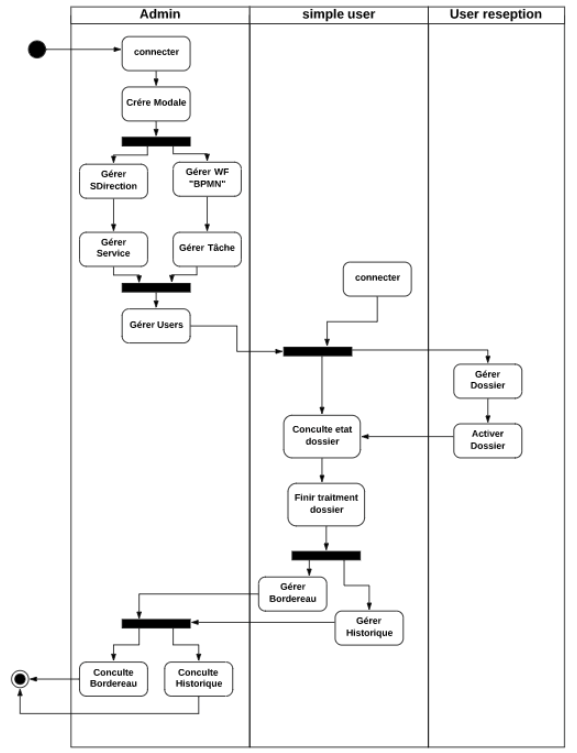
\includegraphics[width=1.1\linewidth]{Dactiviti}
   	\caption{Diagramme d'activité qui  montre interaction des  utilisateurs   en fonction de leurs rôles dans le système en général.}
   	\label{fig:dactiviti}
   \end{figure}
     
   \section{Conclusion}
   
   Dans ce chapitre nous avons fait une étude de notre système logiciel en utilisant la modélisation UML après la spécification des besoins.
   
     Dans le chapitre suivant nous allons expliquer la phase de réalisation du système, son intégration et son déploiement sur le  cloud par les micro service, tout en respectant les directives de la conception.
    
   
 

 \printbibliography


\end{document}
